% Options for packages loaded elsewhere
\PassOptionsToPackage{unicode}{hyperref}
\PassOptionsToPackage{hyphens}{url}
%
\documentclass[
]{book}
\usepackage{amsmath,amssymb}
\usepackage{lmodern}
\usepackage{iftex}
\ifPDFTeX
  \usepackage[T1]{fontenc}
  \usepackage[utf8]{inputenc}
  \usepackage{textcomp} % provide euro and other symbols
\else % if luatex or xetex
  \usepackage{unicode-math}
  \defaultfontfeatures{Scale=MatchLowercase}
  \defaultfontfeatures[\rmfamily]{Ligatures=TeX,Scale=1}
\fi
% Use upquote if available, for straight quotes in verbatim environments
\IfFileExists{upquote.sty}{\usepackage{upquote}}{}
\IfFileExists{microtype.sty}{% use microtype if available
  \usepackage[]{microtype}
  \UseMicrotypeSet[protrusion]{basicmath} % disable protrusion for tt fonts
}{}
\makeatletter
\@ifundefined{KOMAClassName}{% if non-KOMA class
  \IfFileExists{parskip.sty}{%
    \usepackage{parskip}
  }{% else
    \setlength{\parindent}{0pt}
    \setlength{\parskip}{6pt plus 2pt minus 1pt}}
}{% if KOMA class
  \KOMAoptions{parskip=half}}
\makeatother
\usepackage{xcolor}
\usepackage{color}
\usepackage{fancyvrb}
\newcommand{\VerbBar}{|}
\newcommand{\VERB}{\Verb[commandchars=\\\{\}]}
\DefineVerbatimEnvironment{Highlighting}{Verbatim}{commandchars=\\\{\}}
% Add ',fontsize=\small' for more characters per line
\usepackage{framed}
\definecolor{shadecolor}{RGB}{248,248,248}
\newenvironment{Shaded}{\begin{snugshade}}{\end{snugshade}}
\newcommand{\AlertTok}[1]{\textcolor[rgb]{0.94,0.16,0.16}{#1}}
\newcommand{\AnnotationTok}[1]{\textcolor[rgb]{0.56,0.35,0.01}{\textbf{\textit{#1}}}}
\newcommand{\AttributeTok}[1]{\textcolor[rgb]{0.77,0.63,0.00}{#1}}
\newcommand{\BaseNTok}[1]{\textcolor[rgb]{0.00,0.00,0.81}{#1}}
\newcommand{\BuiltInTok}[1]{#1}
\newcommand{\CharTok}[1]{\textcolor[rgb]{0.31,0.60,0.02}{#1}}
\newcommand{\CommentTok}[1]{\textcolor[rgb]{0.56,0.35,0.01}{\textit{#1}}}
\newcommand{\CommentVarTok}[1]{\textcolor[rgb]{0.56,0.35,0.01}{\textbf{\textit{#1}}}}
\newcommand{\ConstantTok}[1]{\textcolor[rgb]{0.00,0.00,0.00}{#1}}
\newcommand{\ControlFlowTok}[1]{\textcolor[rgb]{0.13,0.29,0.53}{\textbf{#1}}}
\newcommand{\DataTypeTok}[1]{\textcolor[rgb]{0.13,0.29,0.53}{#1}}
\newcommand{\DecValTok}[1]{\textcolor[rgb]{0.00,0.00,0.81}{#1}}
\newcommand{\DocumentationTok}[1]{\textcolor[rgb]{0.56,0.35,0.01}{\textbf{\textit{#1}}}}
\newcommand{\ErrorTok}[1]{\textcolor[rgb]{0.64,0.00,0.00}{\textbf{#1}}}
\newcommand{\ExtensionTok}[1]{#1}
\newcommand{\FloatTok}[1]{\textcolor[rgb]{0.00,0.00,0.81}{#1}}
\newcommand{\FunctionTok}[1]{\textcolor[rgb]{0.00,0.00,0.00}{#1}}
\newcommand{\ImportTok}[1]{#1}
\newcommand{\InformationTok}[1]{\textcolor[rgb]{0.56,0.35,0.01}{\textbf{\textit{#1}}}}
\newcommand{\KeywordTok}[1]{\textcolor[rgb]{0.13,0.29,0.53}{\textbf{#1}}}
\newcommand{\NormalTok}[1]{#1}
\newcommand{\OperatorTok}[1]{\textcolor[rgb]{0.81,0.36,0.00}{\textbf{#1}}}
\newcommand{\OtherTok}[1]{\textcolor[rgb]{0.56,0.35,0.01}{#1}}
\newcommand{\PreprocessorTok}[1]{\textcolor[rgb]{0.56,0.35,0.01}{\textit{#1}}}
\newcommand{\RegionMarkerTok}[1]{#1}
\newcommand{\SpecialCharTok}[1]{\textcolor[rgb]{0.00,0.00,0.00}{#1}}
\newcommand{\SpecialStringTok}[1]{\textcolor[rgb]{0.31,0.60,0.02}{#1}}
\newcommand{\StringTok}[1]{\textcolor[rgb]{0.31,0.60,0.02}{#1}}
\newcommand{\VariableTok}[1]{\textcolor[rgb]{0.00,0.00,0.00}{#1}}
\newcommand{\VerbatimStringTok}[1]{\textcolor[rgb]{0.31,0.60,0.02}{#1}}
\newcommand{\WarningTok}[1]{\textcolor[rgb]{0.56,0.35,0.01}{\textbf{\textit{#1}}}}
\usepackage{longtable,booktabs,array}
\usepackage{calc} % for calculating minipage widths
% Correct order of tables after \paragraph or \subparagraph
\usepackage{etoolbox}
\makeatletter
\patchcmd\longtable{\par}{\if@noskipsec\mbox{}\fi\par}{}{}
\makeatother
% Allow footnotes in longtable head/foot
\IfFileExists{footnotehyper.sty}{\usepackage{footnotehyper}}{\usepackage{footnote}}
\makesavenoteenv{longtable}
\usepackage{graphicx}
\makeatletter
\def\maxwidth{\ifdim\Gin@nat@width>\linewidth\linewidth\else\Gin@nat@width\fi}
\def\maxheight{\ifdim\Gin@nat@height>\textheight\textheight\else\Gin@nat@height\fi}
\makeatother
% Scale images if necessary, so that they will not overflow the page
% margins by default, and it is still possible to overwrite the defaults
% using explicit options in \includegraphics[width, height, ...]{}
\setkeys{Gin}{width=\maxwidth,height=\maxheight,keepaspectratio}
% Set default figure placement to htbp
\makeatletter
\def\fps@figure{htbp}
\makeatother
\setlength{\emergencystretch}{3em} % prevent overfull lines
\providecommand{\tightlist}{%
  \setlength{\itemsep}{0pt}\setlength{\parskip}{0pt}}
\setcounter{secnumdepth}{5}
\usepackage{booktabs}
\ifLuaTeX
  \usepackage{selnolig}  % disable illegal ligatures
\fi
\usepackage[]{natbib}
\bibliographystyle{plainnat}
\IfFileExists{bookmark.sty}{\usepackage{bookmark}}{\usepackage{hyperref}}
\IfFileExists{xurl.sty}{\usepackage{xurl}}{} % add URL line breaks if available
\urlstyle{same} % disable monospaced font for URLs
% Make links footnotes instead of hotlinks:
\DeclareRobustCommand{\href}[2]{#2\footnote{\url{#1}}}
\hypersetup{
  pdftitle={Fundamental plots for electrophysiological data},
  pdfauthor={Vikram B. Baliga},
  hidelinks,
  pdfcreator={LaTeX via pandoc}}

\title{Fundamental plots for electrophysiological data}
\author{Vikram B. Baliga}
\date{2023-03-13}

\begin{document}
\maketitle

{
\setcounter{tocdepth}{1}
\tableofcontents
}
\hypertarget{about}{%
\chapter{About}\label{about}}

Until this statement is deleted from this page, please consider everything you
see here a work in progress. Ultimately, this site will provide a walkthrough on
how to produce fundamental plots from electrophysiological data. The content
was initialized using a \href{https://bookdown.org/}{bookdown} template; accordingly,
as this site remains in a developmental stage, content from the template may
linger.

The original content written here is intended to instruct trainees in the
Altshuler Lab at the University of British Columbia to take raw recorded data
from electrophysiological examinations and then produce preliminary plots that
help characterize the recorded neural spike data.

To get started, please use the left navigation and work through chapters in
order.

🐢

\hypertarget{citation}{%
\section*{Citation}\label{citation}}
\addcontentsline{toc}{section}{Citation}

TBD

\hypertarget{license}{%
\section*{License}\label{license}}
\addcontentsline{toc}{section}{License}

The content of this work is licensed under CC-BY. For details please see
\href{https://creativecommons.org/licenses/by/4.0/}{this web page} or the LICENSE
file in \href{https://github.com/flightlab/ephys_fundamental_plots}{flightlab/ephys\_fundamental\_plots}.

\hypertarget{preface}{%
\chapter{Preface}\label{preface}}

\hypertarget{r-packages-versioning}{%
\section{R packages \& versioning}\label{r-packages-versioning}}

The R packages listed below will be necessary at some point over the course of
this book. I recommend installing them all now. The block of code below is
designed to first check if each of the listed packages is already installed on
your computer. If any is missing, then an attempt is made to install it from
CRAN. Finally, all of the packages are loaded into the environment.

\begin{Shaded}
\begin{Highlighting}[]
\DocumentationTok{\#\# Specify the packages you\textquotesingle{}ll use in the script}
\NormalTok{packages }\OtherTok{\textless{}{-}} \FunctionTok{c}\NormalTok{(}\StringTok{"tidyverse"}\NormalTok{,}
              \StringTok{"zoo"}\NormalTok{,}
              \StringTok{"gridExtra"}\NormalTok{,}
              \StringTok{"R.matlab"}\NormalTok{,}
              \StringTok{"cowplot"}\NormalTok{,}
              \StringTok{"easystats"}\NormalTok{,}
              \StringTok{"circular"}\NormalTok{,}
              \StringTok{"splines"}\NormalTok{,}
              \StringTok{"MESS"}\NormalTok{, }\DocumentationTok{\#\# area under curve}
              \StringTok{"zoo"} \DocumentationTok{\#\# rolling means}
\NormalTok{)}
\DocumentationTok{\#\# Now for each package listed, first check to see if the package is already}
\DocumentationTok{\#\# installed. If it is installed, it\textquotesingle{}s simply loaded. If not, it\textquotesingle{}s downloaded }
\DocumentationTok{\#\# from CRAN and then installed and loaded.}
\NormalTok{package.check }\OtherTok{\textless{}{-}} \FunctionTok{lapply}\NormalTok{(packages,}
                        \AttributeTok{FUN =} \ControlFlowTok{function}\NormalTok{(x) \{}
                          \ControlFlowTok{if}\NormalTok{ (}\SpecialCharTok{!}\FunctionTok{require}\NormalTok{(x, }\AttributeTok{character.only =} \ConstantTok{TRUE}\NormalTok{)) \{}
                            \FunctionTok{install.packages}\NormalTok{(x, }\AttributeTok{dependencies =} \ConstantTok{TRUE}\NormalTok{)}
                            \FunctionTok{library}\NormalTok{(x, }\AttributeTok{character.only =} \ConstantTok{TRUE}\NormalTok{)}
\NormalTok{                          \}}
\NormalTok{                        \}}
\NormalTok{)}
\end{Highlighting}
\end{Shaded}

I will use the \texttt{sessionInfo()} command to detail the specific versions of
packages I am using (along with other information about my R session). Please
note that I am not suggesting you obtain exactly the same version of each
package listed below. Instead, the information below is meant to help you assess
whether package versioning underlies any trouble you may encounter.

\begin{verbatim}
## R version 4.2.2 (2022-10-31 ucrt)
## Platform: x86_64-w64-mingw32/x64 (64-bit)
## Running under: Windows 10 x64 (build 19045)
## 
## Matrix products: default
## 
## locale:
## [1] LC_COLLATE=English_United States.utf8 
## [2] LC_CTYPE=English_United States.utf8   
## [3] LC_MONETARY=English_United States.utf8
## [4] LC_NUMERIC=C                          
## [5] LC_TIME=English_United States.utf8    
## 
## attached base packages:
## [1] splines   stats     graphics  grDevices utils     datasets  methods  
## [8] base     
## 
## other attached packages:
##  [1] MESS_0.5.9         circular_0.4-95    see_0.7.4          report_0.5.6      
##  [5] parameters_0.20.2  performance_0.10.2 modelbased_0.8.6   insight_0.19.0    
##  [9] effectsize_0.8.3   datawizard_0.6.5   correlation_0.8.3  bayestestR_0.13.0 
## [13] easystats_0.6.0    cowplot_1.1.1      R.matlab_3.7.0     gridExtra_2.3     
## [17] zoo_1.8-11         lubridate_1.9.2    forcats_1.0.0      stringr_1.5.0     
## [21] dplyr_1.1.0        purrr_1.0.1        readr_2.1.4        tidyr_1.3.0       
## [25] tibble_3.1.8       ggplot2_3.4.1      tidyverse_2.0.0   
## 
## loaded via a namespace (and not attached):
##  [1] R.utils_2.12.2     ggstance_0.3.6     yaml_2.3.7         pillar_1.8.1      
##  [5] backports_1.4.1    lattice_0.20-45    glue_1.6.2         digest_0.6.31     
##  [9] polyclip_1.10-4    colorspace_2.1-0   htmltools_0.5.4    Matrix_1.5-1      
## [13] R.oo_1.25.0        pkgconfig_2.0.3    labelled_2.10.0    broom_1.0.3       
## [17] haven_2.5.1        bookdown_0.32      xtable_1.8-4       mvtnorm_1.1-3     
## [21] scales_1.2.1       tweenr_2.0.2       ggforce_0.4.1      tzdb_0.3.0        
## [25] timechange_0.2.0   emmeans_1.8.4-1    farver_2.1.1       generics_0.1.3    
## [29] ellipsis_0.3.2     withr_2.5.0        geepack_1.3.9      cli_3.6.0         
## [33] magrittr_2.0.3     estimability_1.4.1 evaluate_0.20      R.methodsS3_1.8.2 
## [37] fansi_1.0.4        MASS_7.3-58.2      geeM_0.10.1        tools_4.2.2       
## [41] hms_1.1.2          lifecycle_1.0.3    munsell_0.5.0      compiler_4.2.2    
## [45] rlang_1.0.6        grid_4.2.2         ggridges_0.5.4     rstudioapi_0.14   
## [49] mosaicCore_0.9.2.1 rmarkdown_2.20     boot_1.3-28        gtable_0.3.1      
## [53] R6_2.5.1           knitr_1.42         fastmap_1.1.1      utf8_1.2.3        
## [57] ggformula_0.10.2   stringi_1.7.12     Rcpp_1.0.10        vctrs_0.5.2       
## [61] tidyselect_1.2.0   xfun_0.37          coda_0.19-4
\end{verbatim}

\hypertarget{not_in}{%
\section{\texorpdfstring{\texttt{\%not\_in\%}}{\%not\_in\%}}\label{not_in}}

This guide will also rely on this handy function, which you should add to your
code:

\begin{Shaded}
\begin{Highlighting}[]
\StringTok{\textasciigrave{}}\AttributeTok{\%not\_in\%}\StringTok{\textasciigrave{}} \OtherTok{\textless{}{-}} \FunctionTok{Negate}\NormalTok{(}\StringTok{\textasciigrave{}}\AttributeTok{\%in\%}\StringTok{\textasciigrave{}}\NormalTok{)}
\end{Highlighting}
\end{Shaded}

This simple operator allows you to determine if an element does not appear in a
target object.

\hypertarget{spike-sorting}{%
\chapter{Spike sorting}\label{spike-sorting}}

We'll cover how to spike sort using two programs: 1) \href{https://ced.co.uk/products/spkovin}{Spike2} (written
by Tony Lapsansky) and 2) \href{https://neuralynx.com/}{Neuralynx} (written by Eric Press).

The function of spike sorting is to isolate action potentials from the background voltage signal. These methods use the shape of the waveform to detect and distinguish the spiking activity of each neuron recorded by an electrode.

\hypertarget{spike2}{%
\section{Spike2}\label{spike2}}

Written by Tony Lapsansky, February 24, 2023

These instructions assume that you have been given a Spike2 recording file (extension \texttt{.smrx}) and asked to spike sort.

Spike2 includes a detailed description of the program, accessible by clicking
\texttt{Help} → \texttt{Index}

\begin{figure}
\centering
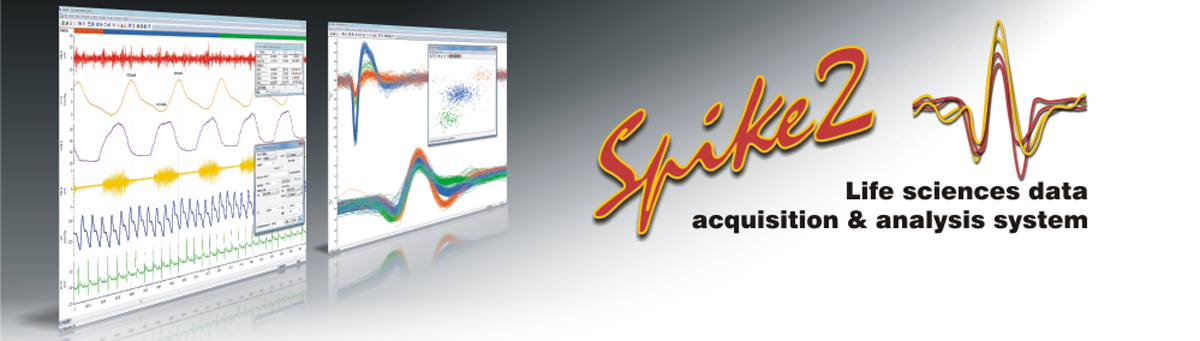
\includegraphics{source_images/sec3.1.1_spike2_banner.png}
\caption{Spike2}
\end{figure}

\hypertarget{file-naming-conventions}{%
\subsection{File naming conventions:}\label{file-naming-conventions}}

\begin{itemize}
\item
  Use the name structure \texttt{YEARMODA\_sequence\_investigator}
\item
  Save data in the corresponding directory
  \texttt{“C:\textbackslash{}InvestigatorName\textbackslash{}ephys\textbackslash{}YEAR-MO-DA”}
\end{itemize}

\hypertarget{spike-sorting-with-spike2}{%
\subsection{Spike sorting with Spike2}\label{spike-sorting-with-spike2}}

\begin{enumerate}
\def\labelenumi{\arabic{enumi}.}
\tightlist
\item
  \textbf{Open the main \texttt{Spike2} file} for the recording. This file should have the
  extension \texttt{.smrx}.
\item
  \textbf{Apply a digital high pass filter}, if needed. Note: if the
  data were collected with the high pass filter set at greater than 100 Hz (no LFP
  signal) then proceed to step 3.

  \begin{itemize}
  \tightlist
  \item
    Right click on the raw data channel (typically Ch1) and select \texttt{FIR\ \ Digital\ Filters…}. We want to use an FIR filter rather than an IIR filter as
    the latter can introduce a variable time lag in the resulting data (see
    Spike 2 \texttt{Help} → \texttt{Index} → \texttt{Digital\ Filter} for full explanation).
  \item
    Under the pull down menu for \texttt{Filter}, change the filter from
    \texttt{Example\ low\ pass\ filter} to \texttt{Example\ high\ pass\ filter}.
  \item
    Select the \texttt{Show\ Details} button in the bottom right.
  \item
    Adjust blue slider change the filter length. Shift the slider until
    the coloured dots above the slider from red to yellow to green. This removes
    wobbles in the data. Use the minimum level (\textasciitilde1019) to achieve green.
    Fine adjustments can be made just under the slider.
    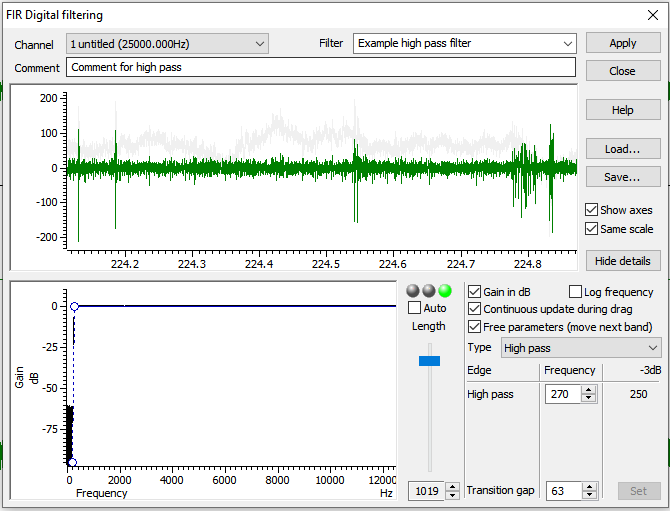
\includegraphics{source_images/sec3.1.1_FIR_filtering.png}
  \item
    Hit \texttt{Apply}
  \item
    Set \texttt{Destination} to the next available channel (typically Channel 4)
  \item
    Click \texttt{Okay}
  \item
    Close the filtering window. You are given the option to save
    the filter. This is unnecessary.
  \end{itemize}
\item
  \textbf{Setting the threshold for spike identification}

  \begin{itemize}
  \tightlist
  \item
    Right click on the filtered channel and select \texttt{New\ WaveMark}
  \item
    Clear previous templates if any are present. To do so, select
    the trash can icon within each template. These may be present
    from a previous session.
  \item
    Locate your cursor position, indicated by the vertical dashed
    line in the main window (typically found at time 0)
  \item
    Slide the dashed line horizontally through the trace to observe potential
    spikes as determined by the default upper and lower thresholds.
  \item
    Right click the upper bound marker (the upper horizontal
    dashed line in the \texttt{WaveMark} window) and select \texttt{Move\ Away}. We will
    rely on the lower bound to identify spikes for sorting, as the activity
    above baseline is typically closer in magnitude to the background.
  \item
    Slide the dashed line horizontally through the trace to observe potential
    spikes as determined by the lower threshold alone.
  \item
    Adjust the lower threshold to catch spikes of interest. This threshold
    will vary based based on the distance between the electrode and the
    neuron, the quality of the isolate, and the level of background noise.
    Values between 50 mV and 200 mV are typical.Set the lower bound so that
    spikes of interest are included and ambiguous spikes are excluded.
  \end{itemize}
\item
  \textbf{Designing the spike template}

  \begin{itemize}
  \tightlist
  \item
    Move the cursor to a characteristic spike. In the upper window, you will
    see the provisional template. Click and hold on the trace in the upper
    window and drag it to the first available spot in the lower, template window.
  \item
    To set parameters for spike sorting, click on the button just to the left
    of the trash can icon (on the top half, upper right of the \texttt{WaveMark}
    window). This is the ``parameters dialog'' button. This opens a template
    settings window.
  \item
    For the line \texttt{Maximum\ amplitude\ change\ for\ a\ match} enter a value between
    \texttt{10} and \texttt{20}. This will allow a spike that fits a template to vary in
    maximum amplitude by up to 10-20\%.
  \item
    For the line \texttt{Remove\ the\ DC\ offset\ before\ template\ matching},
    confirm that the box is checked. This means that Spike2 will account for
    abrupt shifts in the signal baseline before template matching. This is a
    stop-gap for any issues with the digital high pass filter.
  \item
    Click \texttt{OK}.
    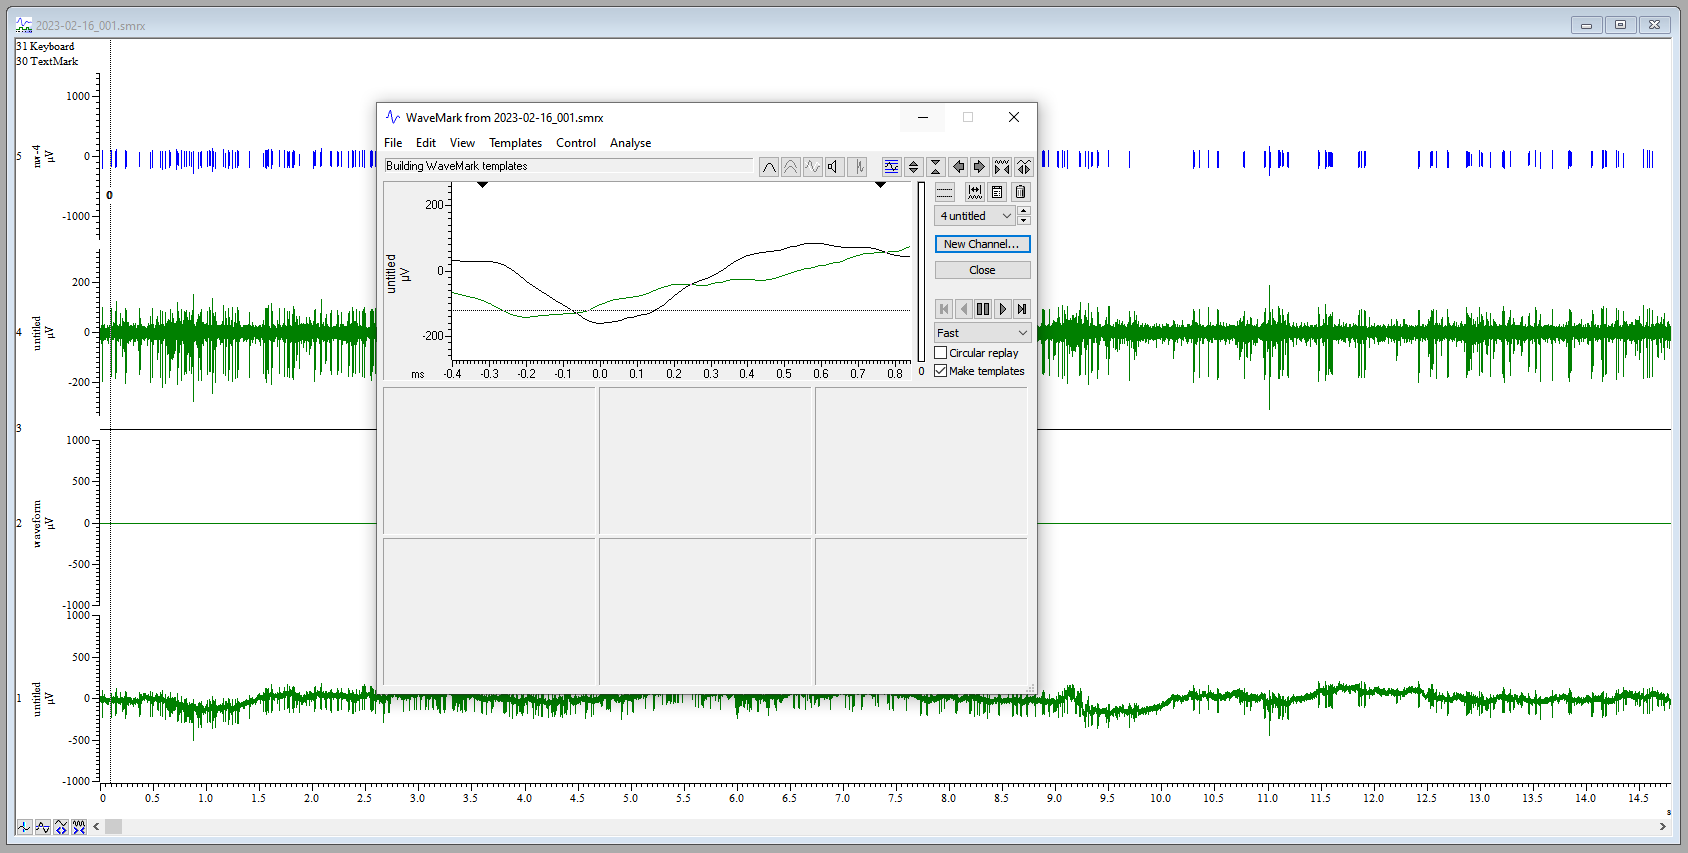
\includegraphics{source_images/sec3.1.1_spike_template.png}
  \end{itemize}
\item
  \textbf{Spike sorting}

  \begin{itemize}
  \tightlist
  \item
    Back in the \texttt{WaveMark} window, make sure that the box
    \texttt{Circular\ replay} is \textbf{unchecked}. If checked, spike sorting will loop
    indefinitely.
  \item
    Ensure that the vertical cursor on the main window is at time
    zero (or the first spike) so that no spikes are missed.
  \item
    Back in the \texttt{WaveMark} window, make sure that the box
    \texttt{Make\ templates} is \textbf{checked}. If unchecked, only spikes corresponding
    to the provisional template will be identified. We want to let spike2
    help us to identify potential multi-unit activity.
  \item
    Hit the play button ▶️, which is called ``run forward''. Spike sorting will
    proceed for several minutes. Each identified spike will appear briefly
    in the \texttt{WaveMark} window and will be assigned to a template.
    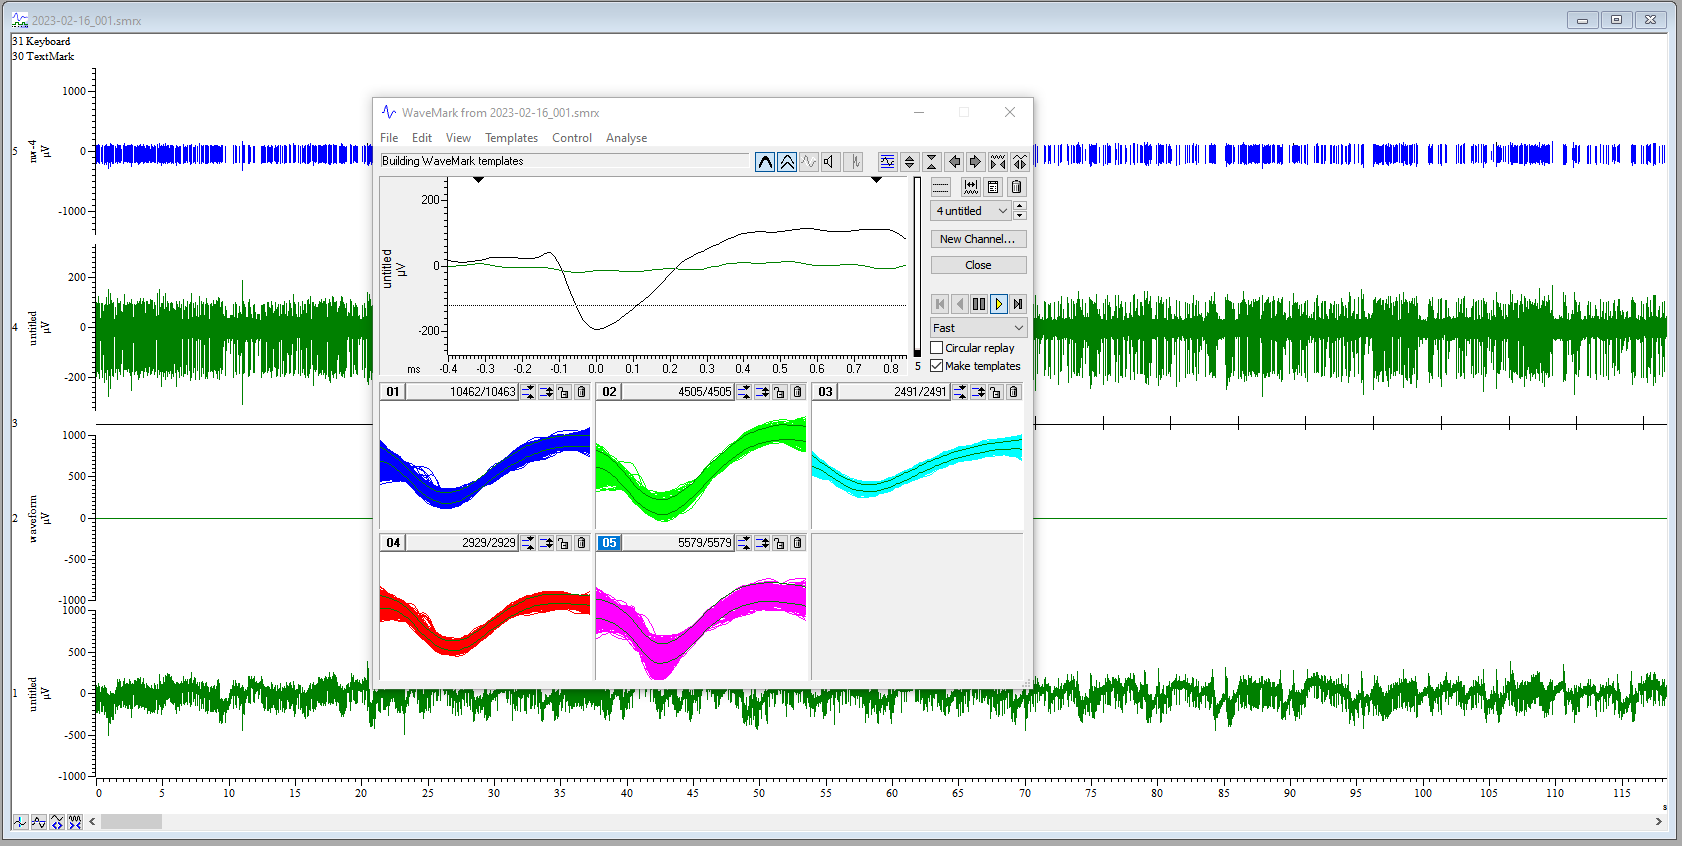
\includegraphics{source_images/sec3.1.1_spike_sorting.png}
    \emph{In this image, I have selected options for \texttt{Overdraw} and \texttt{Show\ template\ limits}}
  \end{itemize}
\item
  \textbf{Merge, delete, and save templates}

  \begin{itemize}
  \tightlist
  \item
    After spike sorting has completed, select \texttt{New\ Channel} on the \texttt{WaveMark} window to place the spike sorted data in the next available channel
    (typically, Channel 5)
  \item
    Close the existing \texttt{WaveMark} window.
  \item
    Right click on the \textbf{spike sorted channel} and select \texttt{Edit\ WaveMark}.
  \item
    Within the \texttt{WaveMark} window, go the pull down menu \texttt{Analyse}
    and select \texttt{Principal\ components}. Select \texttt{OK}. This opens a
    window containing a principal component analysis of all spikes
    colored by their assigned template.
  \item
    Rotate around all three axes to determine if there is one,
    two, or more clusters. In theory, each cluster corresponds to a single
    neuron. Often, spikes are categorized into multiple templates, but
    realistically correspond to the activity of a single neuron.
  \item
    Identify templates that should be deleted and those that
    should be merged. We will delete spikes corresponding to templates that
    are sparse and peripheral.
  \item
    Delete the template(s) in the \texttt{WaveMark} window by selecting
    that template's trash can icon.
  \item
    Merge templates by dragging them into the same window
  \item
    Hit the \texttt{reclassify} button in the \texttt{WaveMark} window to commit these
    changes to the data in the main window.
    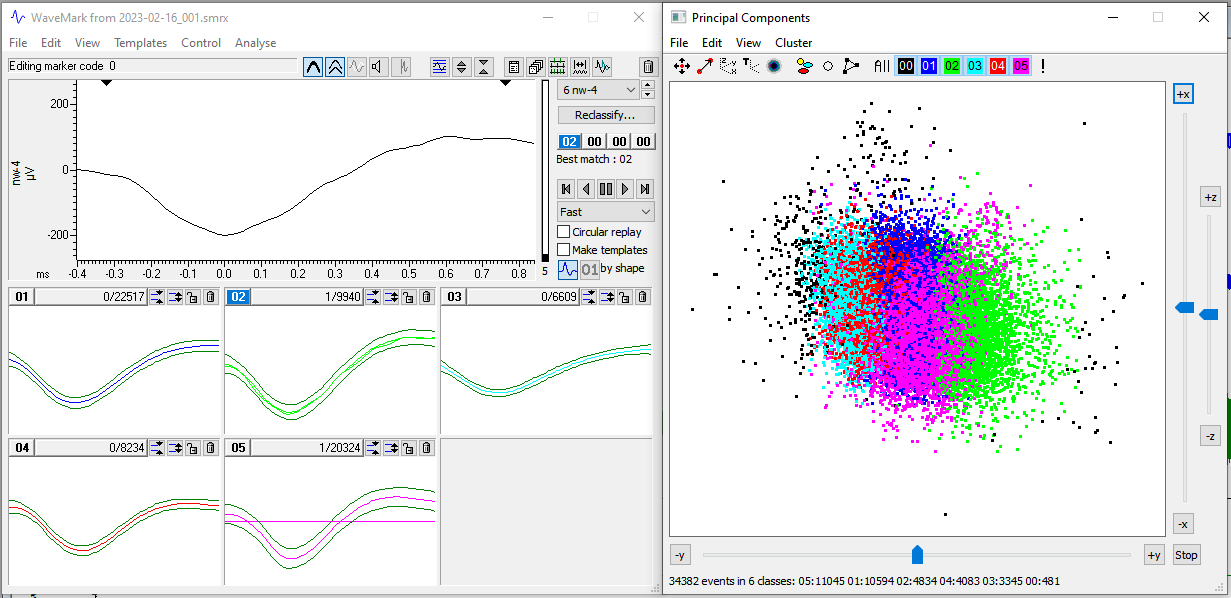
\includegraphics{source_images/sec3.1.1_PCA.png}
    \emph{In this example, we have good evidence from the PCA to merge these five templates.}
  \end{itemize}
\item
  \textbf{Export the spike-sorted data}

  \begin{itemize}
  \tightlist
  \item
    \texttt{File\ →\ Export\ As}
  \item
    Select \texttt{.mat} (\texttt{matlab} data)
  \item
    Use the same filename and location but with the \texttt{.mat}
    extension.
  \item
    Hit \texttt{Save}
  \item
    Select \texttt{Add} for \texttt{All\ Channels}
  \item
    Click \texttt{Export}
  \item
    Click \texttt{OK} (this will take several minutes)
  \end{itemize}
\end{enumerate}

\emph{Note: May need to select an earlier MATLAB file convention to work with R.}

\hypertarget{neuralynx}{%
\section{Neuralynx}\label{neuralynx}}

Written by Eric Press, November 11, 2022

\begin{enumerate}
\def\labelenumi{\arabic{enumi}.}
\tightlist
\item
  Spike sorting database:

  \begin{enumerate}
  \def\labelenumii{\arabic{enumii}.}
  \tightlist
  \item
    Check the column labelled \texttt{Sorting\ status} to find days of
    recording that are \texttt{cued} meaning they are ready to be sorted.
    Recordings are cued for spike sorting once information about
    the recording has been added to the database. This includes
    observations from the day's recording, whether the electrode
    position was moved from the previous recording, and the
    stimulus condition for each recording. The recordings are
    stored at the following location and are named/organized by
    date and time of recording:\\
    \texttt{Computer/LaCie\ (D:)/Eric’s\ data/nlx\_recordings}
  \end{enumerate}
\item
  Filtering the raw traces (CSCs):

  \begin{enumerate}
  \def\labelenumii{\arabic{enumii}.}
  \tightlist
  \item
    Use the \texttt{NlxCSCFiltering} tool on any Windows machine to run a
    band-pass filter on input \texttt{CSC} files.
  \item
    Choose all the \texttt{CSC} files for a given recording, change the
    \texttt{PreAppend} field to \texttt{spfilt}, which stands for spike-filtered
    and adjust the \texttt{DSP} filtering fields to match the image to
    the right. This selects for frequencies in the raw traces
    where spikes will be found, but removes low frequency (LFP)
    and high frequency components of the traces.
    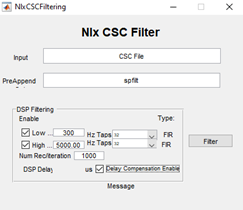
\includegraphics{source_images/sec3.2.1_nix_csc_filter.png}
  \end{enumerate}
\item
  Examine the filtered traces:

  \begin{enumerate}
  \def\labelenumii{\arabic{enumii}.}
  \tightlist
  \item
    Take a closer look at the filtered traces (Open in \texttt{Neuraview}
    on any Windows machine) and determine which channels are
    likely to have isolatable spikes and how many distinct spikes
    there might be. It helps to keep \texttt{Neuraview} open when setting
    thresholds in the next step.
  \end{enumerate}
\item
  Spike detection from filtered traces:

  \begin{enumerate}
  \def\labelenumii{\arabic{enumii}.}
  \tightlist
  \item
    Use the \texttt{CSCSpikeExtractor} tool on any Windows machine to
    detect spikes above or below a given µV) threshold. The units
    displayed in the program will be AdBitVolts which are simply
    10.92x from the µV value.
  \item
    Based on the filtered traces, within \texttt{CSCSpikeExtractor}, set
    the spike extraction properties
    (\texttt{Spike\ Extraction\ -\textgreater{}\ Properties} OR \texttt{Ctrl+P}) as shown above.
    The \texttt{Extraction\ Value} is set to 10.92x the µV you chose by
    viewing the filtered traces.
  \item
    Press \texttt{Ctrl+S} to extract spikes from the selected file at the
    desired settings. The resulting file will be placed in the
    \texttt{extracted\ spikes} filter on the \texttt{Desktop}.
  \item
    Create subfolders in the recording folder for each threshold
    and move the extracted spikes at each threshold into the
    appropriate folder. These spike-detected files will be used
    for spike sorting in the next step.
  \item
    \textbf{If it helps with detecting real spike waveforms while
    eliminating noise, run recordings through spike detection at
    multiple threshold (positive or negative) such that only all
    putative neurons are accounted for a minimal noise is
    detected.}
    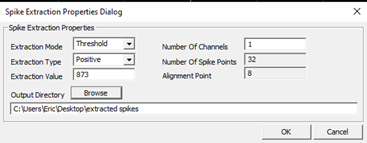
\includegraphics{source_images/sec3.2.2_spike_extraction_properties.png}
  \end{enumerate}
\item
  Spike sorting:

  \begin{enumerate}
  \def\labelenumii{\arabic{enumii}.}
  \tightlist
  \item
    Open the extracted spikes in \texttt{Spikesort3D} on either the
    Neuralynx machine or another Windows machine that has an
    active \texttt{SpikeSort3D} licence. You can also use \texttt{TeamViewer} to
    control the Neuralynx machine but this works much better with
    another Windows machine.
  \item
    Press OK when the feature selection window appears. If you
    want to select alternate features to display, select them from
    the list provided. Sometimes it can be helpful to use PCA1 --
    3 in isolating neurons but often it makes things more
    challenging.
  \item
    Using the 3D Plot, examine the clustering of spikes. Follow
    the image below to aid in interacting with the 3D plot (MB =
    the scroll wheel button i.e.~middle mouse button). You can
    change the features displayed on each axis with \texttt{Q/W}, \texttt{A/S},
    and \texttt{Z/X} respectively. Also, \texttt{Ctrl+P} brings up a window that
    allows you to change the size and opacity of points on the
    plot (I find \texttt{size\ =\ 2}, \texttt{alpha\ =\ 0.5} works well to improve
    visual definition of the clusters). If distinct clusters are
    difficult to see, find the combination of 3 features that
    produces the most noticeable clustering or the greatest spread
    of points in the space. The features displayed in the 3D plot
    are shown at the top left of the plot (i.e.~X(3) Height \# \#
    \# \#). Use those features for the next step.
    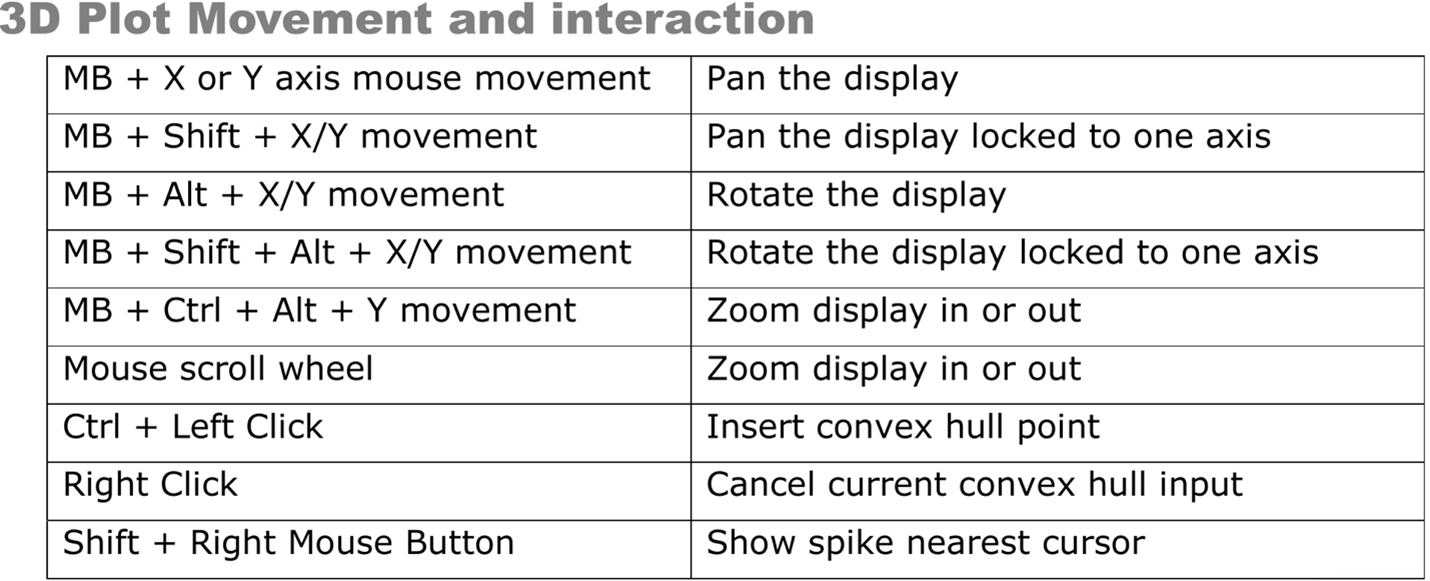
\includegraphics{source_images/sec3.2.3_3d_plot_movement.png}
  \item
    Run \texttt{KlustaKwik} (\texttt{Cluster\ →\ Autocluster\ using\ KlustaKwik})
    and select the 3 features that generate the most clearly
    separable clusters on the 3D view -- often, the first 3
    (\texttt{Peak}, \texttt{Valley}, \texttt{Energy}) do a decent job. Change the
    \texttt{MaxPossibleClusters} to \texttt{10} before pressing \texttt{Run}. The
    remaining settings should match the image below.
    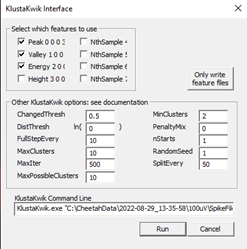
\includegraphics{source_images/sec3.2.4_klustakwik.png}
  \item
    Following calculations, use the \texttt{Waveform} window and the 3D
    plot to group the distinct clusters into what you believe are
    waveforms produced by distinct neurons. Use the number keys to
    highlight distinct clusters and \texttt{Ctrl+M} to merge clusters
    together. \texttt{Ctrl+C} copies the selected cluster and can be used
    to split a cluster into 2 if you believe portions of the
    cluster belong to distinct putative neurons. This step takes
    some practice. You can use \texttt{Ctrl+Z} to undo only one move.
    Otherwise, you may need to exit without saving and start again
    at step 4. Save with \texttt{Ctrl+S} often and click OK to overwrite
    the file.
  \item
    Once you are satisfied with the waveforms left, note how many
    there are, and whether it seems possible that some of the
    groups belong to the same neuron. Consider what you know about
    excitable membranes to make these decisions. Fill out the
    \texttt{Spike\ Sorting\ Database} with the information used to reach
    this point. This includes, the threshold(s), \# of clusters,
    \# of putative neurons (often 1 less than the \# of clusters
    because it would be a stretch to include the smallest
    amplitude waveform as a distinct, separable neuron), and any
    else to note from performing sorting.
  \item
    Save each cluster to its own spike file
    (\texttt{File\ →\ Save\ Multiple\ Spike\ Files})
  \item
    Open the separate spike files you just created, along with the
    original filtered trace in \texttt{Neuraview}. Scroll along the
    recording and examine if the sorting you performed seems
    believable. Do the spikes in different rows really seem like
    they're different in the filtered trace? Do some spikes not
    seem like real spikes? If anything seems amiss, make the
    appropriate merges in \texttt{SpikeSort3D} before proceding.
  \item
    Export the relevant data from the sorting. Perform the
    following:

    \begin{enumerate}
    \def\labelenumiii{\arabic{enumiii}.}
    \tightlist
    \item
      \texttt{File\ →\ Save\ ASCII\ Timestamp\ Files}
    \item
      \texttt{File\ →\ Save\ Multiple\ Spike\ Files}
    \item
      \texttt{File\ →\ Save\ ASCII\ Avg\ Waveforms}
    \item
      Also, save the file itself with \texttt{Ctrl+S}
    \end{enumerate}
  \item
    Lastly, bring up all the waveforms together on the waveform
    plot. Take a screenshot and save it to the folder where the
    extracted spikes (and now timestamps files) are stored.
  \end{enumerate}
\item
  Moving sorted files to other locations:

  \begin{enumerate}
  \def\labelenumii{\arabic{enumii}.}
  \tightlist
  \item
    Once a chunk of recordings have been sorted, copy/paste the
    entire recording file to Eric's orange 1TB storage drive
    (Lacie). Place them in the following folder:
    \texttt{Eric\textquotesingle{}s\ data/sorted\_recordings}
  \end{enumerate}
\end{enumerate}

\hypertarget{raw-data-and-spike-sorted-traces}{%
\chapter{Raw data and spike sorted traces}\label{raw-data-and-spike-sorted-traces}}

Coming soon

\hypertarget{data-wrangling}{%
\chapter{Data wrangling}\label{data-wrangling}}

Once data have been spike sorted, we are ready to begin working in
\texttt{R}. To get to a point where meaningful preliminary plots can be
produced, a few things need to be addressed:

\begin{enumerate}
\def\labelenumi{\arabic{enumi})}
\item
  Labeling the time series of spike \& photodiode data based on the
  stimulus that appears on screen (i.e., matching the log file to
  the data file). This includes labeling phases (like ``blank'',
  ``stationary'', and ``moving'') along with experimental metadata such
  as SF, TF, and stimulus orientation (direction).
\item
  Re-organizing the spike \& photodiode so that separate replicates
  of a stimulus run are uniquely labelled and then arranged
  together.
\item
  Binning the data into 10- and 100-ms data sets, and then exporting
  CSVs of the unbinned, 10-ms-binned, and 100-ms-binned data. This
  will be highly useful for situations where you are handling
  multiple data files (e.g., from different recording days), in
  which case it is likely that your machine will not be able to
  store all objects in RAM.
\end{enumerate}

\begin{quote}
Before proceeding any further, please ensure you have installed and
loaded all the necessary \texttt{R} packages as detailed in the Preface
section of this guide.
\end{quote}

\hypertarget{import-example-file-and-metadata}{%
\section{Import example file and metadata}\label{import-example-file-and-metadata}}

We will use a recently-collected data file and its corresponding
metadata file to showcase the fundamentals of wrangling ephys data
into a more easily plot-able format.

\hypertarget{identify-files-to-import}{%
\subsection{Identify files to import}\label{identify-files-to-import}}

The following code is based on the assumptions that:

\begin{enumerate}
\def\labelenumi{\arabic{enumi})}
\item
  Your files are stored in a directory entitled \texttt{/data}
\item
  The basename of each file (i.e., the name of the file, excluding the file
  extension) is identical for each set of spike sorted data and corresponding
  metadata log file (e.g., \texttt{2023-02-16\_001.mat} and \texttt{2023-02-16\_001.csv} have the
  same basename, which is \texttt{2023-02-16\_001}).
\end{enumerate}

\begin{Shaded}
\begin{Highlighting}[]
\DocumentationTok{\#\# List all files of each file type}
\NormalTok{csv\_files }\OtherTok{\textless{}{-}}
  \FunctionTok{list.files}\NormalTok{(}\StringTok{"./data"}\NormalTok{, }\AttributeTok{pattern =} \StringTok{".csv"}\NormalTok{,}
             \AttributeTok{full.names =} \ConstantTok{TRUE}\NormalTok{)}
\NormalTok{mat\_files }\OtherTok{\textless{}{-}}
  \FunctionTok{list.files}\NormalTok{(}\StringTok{"./data"}\NormalTok{, }\AttributeTok{pattern =} \StringTok{".mat"}\NormalTok{,}
             \AttributeTok{full.names =} \ConstantTok{TRUE}\NormalTok{)}

\DocumentationTok{\#\# Generate metadata tibbles for each file type}
\NormalTok{csv\_file\_info }\OtherTok{\textless{}{-}}
  \FunctionTok{tibble}\NormalTok{(}
    \AttributeTok{csv\_files =}\NormalTok{ csv\_files,}
    \DocumentationTok{\#\# Extract the basename by removing the file extension}
    \AttributeTok{basename =}  \FunctionTok{basename}\NormalTok{(csv\_files) }\SpecialCharTok{\%\textgreater{}\%} \FunctionTok{str\_remove}\NormalTok{(}\StringTok{".csv"}\NormalTok{),}
    \DocumentationTok{\#\# }\AlertTok{NOTE}\DocumentationTok{: PLEASE ADJUST THE FOLLOWING LINE TO BE ABLE TO EXCTRACT OUT THE}
    \DocumentationTok{\#\# DATE BASED ON YOUR NAMING CONVENTION}
    \AttributeTok{basedate =}  \FunctionTok{basename}\NormalTok{(csv\_files) }\SpecialCharTok{\%\textgreater{}\%} \FunctionTok{str\_sub}\NormalTok{(}\AttributeTok{start =} \DecValTok{1}\NormalTok{, }\AttributeTok{end =} \DecValTok{12}\NormalTok{)}
\NormalTok{  )}
\NormalTok{mat\_file\_info }\OtherTok{\textless{}{-}}
  \FunctionTok{tibble}\NormalTok{(}
    \AttributeTok{mat\_files =}\NormalTok{ mat\_files,}
    \DocumentationTok{\#\# Extract the basename by removing the file extension}
    \AttributeTok{basename =}  \FunctionTok{basename}\NormalTok{(mat\_files) }\SpecialCharTok{\%\textgreater{}\%} \FunctionTok{str\_remove}\NormalTok{(}\StringTok{".mat"}\NormalTok{),}
    \DocumentationTok{\#\# }\AlertTok{NOTE}\DocumentationTok{: AGAIN, PLEASE ADJUST THE FOLLOWING LINE TO BE ABLE TO EXCTRACT OUT}
    \DocumentationTok{\#\# THE DATE BASED ON YOUR NAMING CONVENTION}
    \AttributeTok{basedate =}  \FunctionTok{basename}\NormalTok{(mat\_files) }\SpecialCharTok{\%\textgreater{}\%} \FunctionTok{str\_sub}\NormalTok{(}\AttributeTok{start =} \DecValTok{1}\NormalTok{, }\AttributeTok{end =} \DecValTok{12}\NormalTok{)}
\NormalTok{  )}

\DocumentationTok{\#\# Matchmake between .MAT data and .CSV log files}
\NormalTok{csv\_mat\_filejoin }\OtherTok{\textless{}{-}}
  \FunctionTok{inner\_join}\NormalTok{(csv\_file\_info, mat\_file\_info, }\AttributeTok{by =} \StringTok{"basename"}\NormalTok{) }\SpecialCharTok{\%\textgreater{}\%}
  \DocumentationTok{\#\# OPTIONAL STEP: remove any rows where either the .MAT or .CSV is missing}
  \FunctionTok{drop\_na}\NormalTok{()}

\DocumentationTok{\#\# Store a vector of basenames in the environment. This will become useful later}
\NormalTok{base\_names }\OtherTok{\textless{}{-}}\NormalTok{ csv\_mat\_filejoin}\SpecialCharTok{$}\NormalTok{basename}

\DocumentationTok{\#\# Your end products from this code block should look something like:}
\NormalTok{csv\_mat\_filejoin}
\end{Highlighting}
\end{Shaded}

\begin{verbatim}
## # A tibble: 1 x 5
##   csv_files                 basename       basedate.x   mat_files        based~1
##   <chr>                     <chr>          <chr>        <chr>            <chr>  
## 1 ./data/2023-02-16_001.csv 2023-02-16_001 2023-02-16_0 ./data/2023-02-~ 2023-0~
## # ... with abbreviated variable name 1: basedate.y
\end{verbatim}

\begin{Shaded}
\begin{Highlighting}[]
\DocumentationTok{\#\# and:}
\NormalTok{base\_names}
\end{Highlighting}
\end{Shaded}

\begin{verbatim}
## [1] "2023-02-16_001"
\end{verbatim}

\hypertarget{data-import-and-preliminary-labeling}{%
\subsection{Data import and preliminary labeling}\label{data-import-and-preliminary-labeling}}

We will now use the \texttt{R.matlab} package to import the \texttt{.mat} file into
R and then label the spike and photodiode time series based on the
information in the \texttt{.csv} log file

Because \texttt{.mat} files can be large, data import can take several
minutes.

Please see in-line comments for further guidance

\begin{Shaded}
\begin{Highlighting}[]
\DocumentationTok{\#\# Set up empty vectors that will collect sets of replicates that we will be}
\DocumentationTok{\#\# splitting up}
\NormalTok{metadata\_sets }\OtherTok{\textless{}{-}} \ConstantTok{NULL}
\NormalTok{meta\_splits }\OtherTok{\textless{}{-}} \ConstantTok{NULL}
\NormalTok{data\_splits }\OtherTok{\textless{}{-}} \ConstantTok{NULL}
\FunctionTok{gc}\NormalTok{()}
\end{Highlighting}
\end{Shaded}

\begin{verbatim}
##           used  (Mb) gc trigger  (Mb) max used  (Mb)
## Ncells 2425998 129.6    4180621 223.3  4180621 223.3
## Vcells 4197081  32.1   10146329  77.5  8189288  62.5
\end{verbatim}

\begin{Shaded}
\begin{Highlighting}[]
\NormalTok{starttime }\OtherTok{\textless{}{-}} \FunctionTok{Sys.time}\NormalTok{() }\DocumentationTok{\#\# Optional, will help you assess run time}
\ControlFlowTok{for}\NormalTok{ (i }\ControlFlowTok{in} \DecValTok{1}\SpecialCharTok{:}\FunctionTok{nrow}\NormalTok{(csv\_mat\_filejoin)) \{}

  \DocumentationTok{\#\# Which file \# are we working on?}
  \FunctionTok{print}\NormalTok{(i)}

  \DocumentationTok{\#\# Set up temporary objects in which to eventually write data}
\NormalTok{  csv\_data\_sets }\OtherTok{\textless{}{-}} \ConstantTok{NULL}
\NormalTok{  mat\_data\_sets }\OtherTok{\textless{}{-}} \ConstantTok{NULL}
\NormalTok{  joined\_data\_sets }\OtherTok{\textless{}{-}} \ConstantTok{NULL}

  \DocumentationTok{\#\# Import the matlab file. This may take some time}
\NormalTok{  mat\_import }\OtherTok{\textless{}{-}}
\NormalTok{    R.matlab}\SpecialCharTok{::}\FunctionTok{readMat}\NormalTok{(csv\_mat\_filejoin[i,}\StringTok{"mat\_files"}\NormalTok{])}

  \DocumentationTok{\#\# Read in the corresponding csv log file}
\NormalTok{  csv\_data\_sets[[i]] }\OtherTok{\textless{}{-}}
    \FunctionTok{read\_csv}\NormalTok{(}\FunctionTok{as.character}\NormalTok{(csv\_mat\_filejoin[i,}\StringTok{"csv\_files"}\NormalTok{]),}
             \AttributeTok{show\_col\_types =} \ConstantTok{FALSE}\NormalTok{) }\SpecialCharTok{\%\textgreater{}\%}
    \DocumentationTok{\#\# Rename columns for convenience}
    \FunctionTok{rename}\NormalTok{(}
      \AttributeTok{Spatial\_Frequency =} \StringTok{\textasciigrave{}}\AttributeTok{Spatial Frequency}\StringTok{\textasciigrave{}}\NormalTok{,}
      \AttributeTok{Temporal\_Frequency =} \StringTok{\textasciigrave{}}\AttributeTok{Temporal Frequency}\StringTok{\textasciigrave{}}\NormalTok{,}
      \AttributeTok{Cycles\_Per\_Pixel =} \StringTok{\textasciigrave{}}\AttributeTok{Cycles Per Pixel}\StringTok{\textasciigrave{}}
\NormalTok{    )}

  \DocumentationTok{\#\# The log file does not have time = 0, so set up a separate tibble to}
  \DocumentationTok{\#\# add this info in later. Some of the metadata will just be filler for now.}
\NormalTok{  initial }\OtherTok{\textless{}{-}} \FunctionTok{tibble}\NormalTok{(}
    \AttributeTok{Trial =} \StringTok{"initialization"}\NormalTok{,}
    \AttributeTok{Spatial\_Frequency =}\NormalTok{  csv\_data\_sets[[i]]}\SpecialCharTok{$}\NormalTok{Spatial\_Frequency[}\DecValTok{1}\NormalTok{],}
    \AttributeTok{Cycles\_Per\_Pixel  =}\NormalTok{  csv\_data\_sets[[i]]}\SpecialCharTok{$}\NormalTok{Cycles\_Per\_Pixel[}\DecValTok{1}\NormalTok{],}
    \AttributeTok{Temporal\_Frequency =}\NormalTok{ csv\_data\_sets[[i]]}\SpecialCharTok{$}\NormalTok{Temporal\_Frequency[}\DecValTok{1}\NormalTok{],}
    \AttributeTok{Direction  =}\NormalTok{ csv\_data\_sets[[i]]}\SpecialCharTok{$}\NormalTok{Direction[}\DecValTok{1}\NormalTok{],}
    \AttributeTok{Time =} \FloatTok{0.000}
\NormalTok{  )}

  \DocumentationTok{\#\# Find photodiode}
  \DocumentationTok{\#\# It is almost always in channel 2, but we should be sure to check before}
  \DocumentationTok{\#\# extracting automatically}
\NormalTok{  photod\_default\_channel }\OtherTok{\textless{}{-}}
\NormalTok{    mat\_import[[stringr}\SpecialCharTok{::}\FunctionTok{str\_which}\NormalTok{(}\FunctionTok{names}\NormalTok{(mat\_import), }\StringTok{"Ch2"}\NormalTok{)[}\DecValTok{1}\NormalTok{]]]}
  \ControlFlowTok{if}\NormalTok{ (}\SpecialCharTok{!}\NormalTok{photod\_default\_channel[}\DecValTok{1}\NormalTok{][[}\DecValTok{1}\NormalTok{]][}\DecValTok{1}\NormalTok{] }\SpecialCharTok{==} \StringTok{"waveform"}\NormalTok{) \{}
    \FunctionTok{warning}\NormalTok{(}\StringTok{"File "}\NormalTok{, i,}\StringTok{": Photodiode channel identity uncertain"}\NormalTok{)}
\NormalTok{  \}}

  \DocumentationTok{\#\# Find spikes}
  \DocumentationTok{\#\# Similarly, spikes are almost always in channel 5, but we should check}
\NormalTok{  spikes\_default\_channel }\OtherTok{\textless{}{-}}
\NormalTok{    mat\_import[[stringr}\SpecialCharTok{::}\FunctionTok{str\_which}\NormalTok{(}\FunctionTok{names}\NormalTok{(mat\_import), }\StringTok{"Ch5"}\NormalTok{)[}\DecValTok{1}\NormalTok{]]]}
  \ControlFlowTok{if}\NormalTok{(}\StringTok{"codes"} \SpecialCharTok{\%not\_in\%} \FunctionTok{attributes}\NormalTok{(spikes\_default\_channel)}\SpecialCharTok{$}\NormalTok{dimnames[[}\DecValTok{1}\NormalTok{]]) \{}
    \FunctionTok{warning}\NormalTok{(}\StringTok{"File "}\NormalTok{, i,}\StringTok{": Sorted spikes channel identity uncertain"}\NormalTok{)}
\NormalTok{  \}}
  \DocumentationTok{\#\# If that worked, see if we can automatically determine the "times" and}
  \DocumentationTok{\#\# "codes" slot numbers}
\NormalTok{  times\_location }\OtherTok{\textless{}{-}}
    \FunctionTok{which}\NormalTok{(}\FunctionTok{attributes}\NormalTok{(spikes\_default\_channel)}\SpecialCharTok{$}\NormalTok{dimnames[[}\DecValTok{1}\NormalTok{]] }\SpecialCharTok{==} \StringTok{"times"}\NormalTok{)}
\NormalTok{  codes\_location }\OtherTok{\textless{}{-}}
    \FunctionTok{which}\NormalTok{(}\FunctionTok{attributes}\NormalTok{(spikes\_default\_channel)}\SpecialCharTok{$}\NormalTok{dimnames[[}\DecValTok{1}\NormalTok{]] }\SpecialCharTok{==} \StringTok{"codes"}\NormalTok{)}

  \DocumentationTok{\#\# Find matlab\textquotesingle{}s stimulus change log}
\NormalTok{  stim\_change\_channel }\OtherTok{\textless{}{-}}
\NormalTok{    mat\_import[[stringr}\SpecialCharTok{::}\FunctionTok{str\_which}\NormalTok{(}\FunctionTok{names}\NormalTok{(mat\_import), }\StringTok{"Ch3"}\NormalTok{)[}\DecValTok{1}\NormalTok{]]]}
  \DocumentationTok{\#\# Each sweep should be 5 secs. We\textquotesingle{}ll check that the median is 5}
  \DocumentationTok{\#\# If this results in an error, then the channel identity could be wrong, or}
  \DocumentationTok{\#\# there may have been an issue with sweep duration during the recording}
  \DocumentationTok{\#\# process}
  \ControlFlowTok{if}\NormalTok{(}\SpecialCharTok{!}\FunctionTok{median}\NormalTok{(}\FunctionTok{round}\NormalTok{(}\FunctionTok{diff}\NormalTok{(stim\_change\_channel[[}\DecValTok{5}\NormalTok{]][,}\DecValTok{1}\NormalTok{]),}\DecValTok{0}\NormalTok{)) }\SpecialCharTok{==} \DecValTok{5}\NormalTok{) \{}
    \FunctionTok{warning}\NormalTok{(}\StringTok{"File "}\NormalTok{, i,}\StringTok{": stim change channel identity uncertain"}\NormalTok{)}
\NormalTok{  \}}

  \DocumentationTok{\#\# Determine when the onset of motion occurred according to matlab}
\NormalTok{  first\_moving\_mat }\OtherTok{\textless{}{-}}
\NormalTok{    stim\_change\_channel[[}\DecValTok{5}\NormalTok{]][,}\DecValTok{1}\NormalTok{][}\DecValTok{1}\NormalTok{]}
  \DocumentationTok{\#\# Find the first "moving" phase in the log file}
\NormalTok{  first\_moving\_csv }\OtherTok{\textless{}{-}}
\NormalTok{    csv\_data\_sets[[i]] }\SpecialCharTok{\%\textgreater{}\%}
    \FunctionTok{filter}\NormalTok{(Trial }\SpecialCharTok{==} \StringTok{"moving"}\NormalTok{) }\SpecialCharTok{\%\textgreater{}\%}
    \FunctionTok{select}\NormalTok{(Time) }\SpecialCharTok{\%\textgreater{}\%}
    \FunctionTok{slice}\NormalTok{(}\DecValTok{1}\NormalTok{) }\SpecialCharTok{\%\textgreater{}\%}
    \FunctionTok{as.numeric}\NormalTok{()}
  \DocumentationTok{\#\# Find the first "blank" phase in the log file}
\NormalTok{  first\_blank }\OtherTok{\textless{}{-}}
\NormalTok{    csv\_data\_sets[[i]] }\SpecialCharTok{\%\textgreater{}\%}
    \FunctionTok{filter}\NormalTok{(Trial }\SpecialCharTok{==} \StringTok{"blank"}\NormalTok{) }\SpecialCharTok{\%\textgreater{}\%}
    \FunctionTok{select}\NormalTok{(Time) }\SpecialCharTok{\%\textgreater{}\%}
    \FunctionTok{slice}\NormalTok{(}\DecValTok{1}\NormalTok{) }\SpecialCharTok{\%\textgreater{}\%}
    \FunctionTok{as.numeric}\NormalTok{()}
  \DocumentationTok{\#\# Compute the difference between these two}
\NormalTok{  first\_mvbl\_diff }\OtherTok{\textless{}{-}}\NormalTok{ first\_moving\_csv }\SpecialCharTok{{-}}\NormalTok{ first\_blank}

  \DocumentationTok{\#\# Check to see if the final row of the metadata is "moving" and truncate}
  \DocumentationTok{\#\# if not}
  \DocumentationTok{\#\# This can effectively be done by truncating after the final "moving" phase}
\NormalTok{  max\_moving\_sweep }\OtherTok{\textless{}{-}}
    \FunctionTok{max}\NormalTok{(}\FunctionTok{which}\NormalTok{(csv\_data\_sets[[i]]}\SpecialCharTok{$}\NormalTok{Trial }\SpecialCharTok{==} \StringTok{"moving"}\NormalTok{))}

\NormalTok{  first\_csv\_tmp }\OtherTok{\textless{}{-}}
    \FunctionTok{bind\_rows}\NormalTok{(initial, csv\_data\_sets[[i]]) }\SpecialCharTok{\%\textgreater{}\%}
    \DocumentationTok{\#\# Add 1 to max moving sweep since we tacked on "initial" in previous step}
    \DocumentationTok{\#\# Then slice to restrict any extraneous partial sweeps}
    \FunctionTok{slice\_head}\NormalTok{(}\AttributeTok{n =}\NormalTok{ (max\_moving\_sweep }\SpecialCharTok{+} \DecValTok{1}\NormalTok{)) }\SpecialCharTok{\%\textgreater{}\%}
    \DocumentationTok{\#\# Add the first event time to "Time" and subtract first\_mvbl\_diff (\textasciitilde{}2 secs)}
    \DocumentationTok{\#\# What this does is shift the log csv\textquotesingle{}s time stamping to match the matlab}
    \DocumentationTok{\#\# file\textquotesingle{}s stim change channel\textquotesingle{}s time stamping}
    \FunctionTok{mutate}\NormalTok{(}\AttributeTok{Time =}\NormalTok{ Time }\SpecialCharTok{+}\NormalTok{ first\_moving\_mat }\SpecialCharTok{{-}}\NormalTok{ first\_mvbl\_diff }\SpecialCharTok{{-}}\NormalTok{ first\_blank) }\SpecialCharTok{\%\textgreater{}\%}
    \DocumentationTok{\#\# Make character version of Time for joining later}
    \DocumentationTok{\#\# This will be crucial for \_join functions}
    \FunctionTok{mutate}\NormalTok{(}\AttributeTok{Time\_char =} \FunctionTok{as.character}\NormalTok{(}\FunctionTok{round}\NormalTok{(Time,}\DecValTok{3}\NormalTok{)))}

  \DocumentationTok{\#\# Duplicate the initialization for ease of setting T0}
\NormalTok{  inception }\OtherTok{\textless{}{-}}
\NormalTok{    initial }\SpecialCharTok{\%\textgreater{}\%}
    \FunctionTok{mutate}\NormalTok{(}\AttributeTok{Time\_char =} \FunctionTok{as.character}\NormalTok{(}\FunctionTok{round}\NormalTok{(Time,}\DecValTok{3}\NormalTok{)))}
\NormalTok{  inception}\SpecialCharTok{$}\NormalTok{Trial[}\DecValTok{1}\NormalTok{] }\OtherTok{\textless{}{-}} \StringTok{"inception"}

  \DocumentationTok{\#\# Bind the initialization rows}
\NormalTok{  first\_csv }\OtherTok{\textless{}{-}}
    \FunctionTok{bind\_rows}\NormalTok{(inception, first\_csv\_tmp)}
  \DocumentationTok{\#\# Compute stimulus end times}
\NormalTok{  first\_csv}\SpecialCharTok{$}\NormalTok{Stim\_end }\OtherTok{\textless{}{-}} \FunctionTok{c}\NormalTok{(first\_csv}\SpecialCharTok{$}\NormalTok{Time[}\SpecialCharTok{{-}}\DecValTok{1}\NormalTok{], }\FunctionTok{max}\NormalTok{(first\_csv}\SpecialCharTok{$}\NormalTok{Time) }\SpecialCharTok{+} \DecValTok{3}\NormalTok{)}

  \DocumentationTok{\#\# Get final time}
\NormalTok{  final\_time }\OtherTok{\textless{}{-}}\NormalTok{ first\_csv}\SpecialCharTok{$}\NormalTok{Stim\_end[}\FunctionTok{nrow}\NormalTok{(first\_csv)]}

  \DocumentationTok{\#\# Extract photodiode data}
  \DocumentationTok{\#\# First generate a time sequence to match to the photodiode trace}
\NormalTok{  Time\_vec }\OtherTok{\textless{}{-}} \FunctionTok{seq}\NormalTok{(}
    \AttributeTok{from =} \FloatTok{0.0000}\NormalTok{,}
    \AttributeTok{by =} \DecValTok{1} \SpecialCharTok{/} \DecValTok{25000}\NormalTok{,}
    \AttributeTok{length.out =} \FunctionTok{length}\NormalTok{(photod\_default\_channel[}\DecValTok{9}\NormalTok{][[}\DecValTok{1}\NormalTok{]][, }\DecValTok{1}\NormalTok{])}
\NormalTok{  )}
  \DocumentationTok{\#\# The key thing is to get a character version of time from this}
\NormalTok{  Time\_char\_vec }\OtherTok{\textless{}{-}} \FunctionTok{as.character}\NormalTok{(}\FunctionTok{round}\NormalTok{(Time\_vec, }\DecValTok{3}\NormalTok{))}

  \DocumentationTok{\#\# Grab the photodiode data}
\NormalTok{  photod\_full }\OtherTok{\textless{}{-}}
    \FunctionTok{tibble}\NormalTok{(}\AttributeTok{Photod =}
\NormalTok{             photod\_default\_channel[}\DecValTok{9}\NormalTok{][[}\DecValTok{1}\NormalTok{]][, }\DecValTok{1}\NormalTok{])}
  \DocumentationTok{\#\# Add numeric time}
\NormalTok{  photod\_full}\SpecialCharTok{$}\NormalTok{Time }\OtherTok{\textless{}{-}}
    \FunctionTok{seq}\NormalTok{(}
      \AttributeTok{from =} \FloatTok{0.0000}\NormalTok{,}
      \AttributeTok{by =} \DecValTok{1} \SpecialCharTok{/} \DecValTok{25000}\NormalTok{,}
      \AttributeTok{length.out =} \FunctionTok{nrow}\NormalTok{(photod\_full)}
\NormalTok{    )}
  \FunctionTok{options}\NormalTok{(}\AttributeTok{scipen =} \DecValTok{999}\NormalTok{)}
\NormalTok{  photod\_full }\OtherTok{\textless{}{-}}
\NormalTok{    photod\_full }\SpecialCharTok{\%\textgreater{}\%}
    \DocumentationTok{\#\# Add the character time}
    \FunctionTok{add\_column}\NormalTok{(}\AttributeTok{Time\_char =}\NormalTok{ Time\_char\_vec) }\SpecialCharTok{\%\textgreater{}\%}
    \DocumentationTok{\#\# Use the charcter time to define a group}
    \FunctionTok{group\_by}\NormalTok{(Time\_char) }\SpecialCharTok{\%\textgreater{}\%}
    \DocumentationTok{\#\# Then average the photodiode within}
    \FunctionTok{summarise}\NormalTok{(}\AttributeTok{Photod =} \FunctionTok{mean}\NormalTok{(Photod)) }\SpecialCharTok{\%\textgreater{}\%}
    \FunctionTok{ungroup}\NormalTok{() }\SpecialCharTok{\%\textgreater{}\%}
    \FunctionTok{mutate}\NormalTok{(}\AttributeTok{Time =} \FunctionTok{round}\NormalTok{(}\FunctionTok{as.numeric}\NormalTok{(Time\_char), }\DecValTok{3}\NormalTok{)) }\SpecialCharTok{\%\textgreater{}\%}
    \FunctionTok{arrange}\NormalTok{(Time) }\SpecialCharTok{\%\textgreater{}\%}
    \FunctionTok{filter}\NormalTok{(Time }\SpecialCharTok{\textless{}=}\NormalTok{ final\_time)}

  \DocumentationTok{\#\# Extract all spike data}
\NormalTok{  all\_spike\_dat }\OtherTok{\textless{}{-}}
    \FunctionTok{tibble}\NormalTok{(}
      \AttributeTok{Time =}
\NormalTok{        spikes\_default\_channel[times\_location][[}\DecValTok{1}\NormalTok{]][, }\DecValTok{1}\NormalTok{],}
      \AttributeTok{code =}
\NormalTok{        spikes\_default\_channel[codes\_location][[}\DecValTok{1}\NormalTok{]][, }\DecValTok{1}\NormalTok{]) }\SpecialCharTok{\%\textgreater{}\%}
    \DocumentationTok{\#\# Characterize time, for purposes of joining later}
    \FunctionTok{mutate}\NormalTok{(}\AttributeTok{Time\_char =} \FunctionTok{as.character}\NormalTok{(}\FunctionTok{round}\NormalTok{(Time, }\DecValTok{3}\NormalTok{)))}

  \DocumentationTok{\#\# How many distinct neurons are there?}
\NormalTok{  cell\_ids }\OtherTok{\textless{}{-}} \FunctionTok{sort}\NormalTok{(}\FunctionTok{unique}\NormalTok{(all\_spike\_dat}\SpecialCharTok{$}\NormalTok{code))}
\NormalTok{  n\_cells }\OtherTok{\textless{}{-}} \DecValTok{1}\SpecialCharTok{:}\FunctionTok{length}\NormalTok{(cell\_ids)}

  \ControlFlowTok{if}\NormalTok{(}\FunctionTok{length}\NormalTok{(n\_cells) }\SpecialCharTok{\textgreater{}} \DecValTok{1}\NormalTok{) \{ }\DocumentationTok{\#\# if there\textquotesingle{}s more than one distinct neuron}
\NormalTok{    all\_spike\_dat\_tmp }\OtherTok{\textless{}{-}}
\NormalTok{      all\_spike\_dat }\SpecialCharTok{\%\textgreater{}\%}
      \DocumentationTok{\#\# Group by identity of spiking neuron}
      \FunctionTok{group\_by}\NormalTok{(code) }\SpecialCharTok{\%\textgreater{}\%}
      \DocumentationTok{\#\# Split into separate dfs, one per neuron}
      \FunctionTok{group\_split}\NormalTok{()}

    \DocumentationTok{\#\# Additional cells are labeled as "Spike\_n"}
\NormalTok{    all\_cells }\OtherTok{\textless{}{-}} \ConstantTok{NULL}
    \ControlFlowTok{for}\NormalTok{ (j }\ControlFlowTok{in}\NormalTok{ n\_cells) \{}
      \CommentTok{\#print(j)}

\NormalTok{      new\_name }\OtherTok{=} \FunctionTok{paste0}\NormalTok{(}\StringTok{"Spikes\_"}\NormalTok{, cell\_ids[j])}
\NormalTok{      all\_cells[[j]] }\OtherTok{\textless{}{-}}
\NormalTok{        all\_spike\_dat\_tmp[[j]]}

      \DocumentationTok{\#\# Consolidate to 3 decimal places}
\NormalTok{      all\_cells[[j]] }\OtherTok{\textless{}{-}}
\NormalTok{        all\_cells[[j]] }\SpecialCharTok{\%\textgreater{}\%}
        \FunctionTok{group\_by}\NormalTok{(Time\_char) }\SpecialCharTok{\%\textgreater{}\%}
        \FunctionTok{summarise}\NormalTok{(}\AttributeTok{code =} \FunctionTok{mean}\NormalTok{(code)) }\SpecialCharTok{\%\textgreater{}\%}
        \FunctionTok{mutate}\NormalTok{(}\AttributeTok{code =} \FunctionTok{ceiling}\NormalTok{(code)) }\SpecialCharTok{\%\textgreater{}\%}
        \FunctionTok{ungroup}\NormalTok{() }\SpecialCharTok{\%\textgreater{}\%}
        \FunctionTok{mutate}\NormalTok{(}\AttributeTok{Time =} \FunctionTok{round}\NormalTok{(}\FunctionTok{as.numeric}\NormalTok{(Time\_char), }\DecValTok{3}\NormalTok{)) }\SpecialCharTok{\%\textgreater{}\%}
        \FunctionTok{arrange}\NormalTok{(Time) }\SpecialCharTok{\%\textgreater{}\%}
        \FunctionTok{filter}\NormalTok{(Time }\SpecialCharTok{\textless{}=}\NormalTok{ final\_time)}

      \FunctionTok{names}\NormalTok{(all\_cells[[j]])[}\FunctionTok{match}\NormalTok{(}\StringTok{"code"}\NormalTok{, }\FunctionTok{names}\NormalTok{(all\_cells[[j]]))] }\OtherTok{\textless{}{-}}
\NormalTok{        new\_name}
      \DocumentationTok{\#\# Replace "j" with 1 to indicate presence/absence of spike rather than}
      \DocumentationTok{\#\# cell identity}
\NormalTok{      all\_cells[[j]][new\_name] }\OtherTok{\textless{}{-}} \DecValTok{1}

      \DocumentationTok{\#\# If the identity is 1, replace "Spikes\_1" with just "Spikes"}
      \ControlFlowTok{if}\NormalTok{ (new\_name }\SpecialCharTok{==} \StringTok{"Spikes\_1"}\NormalTok{) \{}
        \FunctionTok{names}\NormalTok{(all\_cells[[j]])[}\FunctionTok{match}\NormalTok{(new\_name, }\FunctionTok{names}\NormalTok{(all\_cells[[j]]))] }\OtherTok{\textless{}{-}}
          \StringTok{"Spikes"}
\NormalTok{      \}}
\NormalTok{    \}}

    \DocumentationTok{\#\# Consolidate}
\NormalTok{    all\_spike\_dat }\OtherTok{\textless{}{-}}
\NormalTok{      all\_cells }\SpecialCharTok{\%\textgreater{}\%}
      \DocumentationTok{\#\# Tack on additional spike columns}
      \FunctionTok{reduce}\NormalTok{(full\_join, }\AttributeTok{by =} \StringTok{"Time\_char"}\NormalTok{) }\SpecialCharTok{\%\textgreater{}\%}
      \FunctionTok{arrange}\NormalTok{(Time\_char) }\SpecialCharTok{\%\textgreater{}\%}
      \DocumentationTok{\#\# Remove time.n columns but}
      \DocumentationTok{\#\# Do not remove Time\_char}
      \FunctionTok{select}\NormalTok{(}\SpecialCharTok{{-}}\FunctionTok{contains}\NormalTok{(}\StringTok{"Time."}\NormalTok{)) }\SpecialCharTok{\%\textgreater{}\%}
      \DocumentationTok{\#\# Regenerate numeric time}
      \FunctionTok{mutate}\NormalTok{(}
        \AttributeTok{Time =} \FunctionTok{as.numeric}\NormalTok{(Time\_char)}
\NormalTok{      ) }\SpecialCharTok{\%\textgreater{}\%}
      \FunctionTok{select}\NormalTok{(Time, Time\_char, Spikes, }\FunctionTok{everything}\NormalTok{()) }\SpecialCharTok{\%\textgreater{}\%}
      \FunctionTok{filter}\NormalTok{(Time }\SpecialCharTok{\textless{}=}\NormalTok{ final\_time)}

\NormalTok{  \} }\ControlFlowTok{else}\NormalTok{ \{ }\DocumentationTok{\#\# If there\textquotesingle{}s only 1 neuron}
\NormalTok{    all\_spike\_dat }\OtherTok{\textless{}{-}}
\NormalTok{      all\_spike\_dat }\SpecialCharTok{\%\textgreater{}\%}
      \FunctionTok{group\_by}\NormalTok{(Time\_char) }\SpecialCharTok{\%\textgreater{}\%}
      \FunctionTok{summarise}\NormalTok{(}\AttributeTok{code =} \FunctionTok{mean}\NormalTok{(code)) }\SpecialCharTok{\%\textgreater{}\%}
      \FunctionTok{mutate}\NormalTok{(}\AttributeTok{code =} \FunctionTok{ceiling}\NormalTok{(code)) }\SpecialCharTok{\%\textgreater{}\%}
      \FunctionTok{ungroup}\NormalTok{() }\SpecialCharTok{\%\textgreater{}\%}
      \FunctionTok{rename}\NormalTok{(}\AttributeTok{Spikes =}\NormalTok{ code) }\SpecialCharTok{\%\textgreater{}\%}
      \FunctionTok{mutate}\NormalTok{(}\AttributeTok{Time =} \FunctionTok{round}\NormalTok{(}\FunctionTok{as.numeric}\NormalTok{(Time\_char), }\DecValTok{3}\NormalTok{)) }\SpecialCharTok{\%\textgreater{}\%}
      \FunctionTok{arrange}\NormalTok{(Time) }\SpecialCharTok{\%\textgreater{}\%}
      \FunctionTok{filter}\NormalTok{(Time }\SpecialCharTok{\textless{}=}\NormalTok{ final\_time) }\SpecialCharTok{\%\textgreater{}\%}
      \FunctionTok{select}\NormalTok{(Time, Time\_char, }\FunctionTok{everything}\NormalTok{())}
\NormalTok{  \}}

  \FunctionTok{options}\NormalTok{(}\AttributeTok{scipen =} \DecValTok{999}\NormalTok{)}
\NormalTok{  mat\_data\_sets[[i]] }\OtherTok{\textless{}{-}}
    \DocumentationTok{\#\# Generate a time sequence from 0 to final\_time}
    \FunctionTok{tibble}\NormalTok{(}
      \AttributeTok{Time =} \FunctionTok{seq}\NormalTok{(}\AttributeTok{from =} \DecValTok{0}\NormalTok{, }\AttributeTok{to =}\NormalTok{ final\_time, }\AttributeTok{by =} \FloatTok{0.001}\NormalTok{)}
\NormalTok{    ) }\SpecialCharTok{\%\textgreater{}\%}
    \DocumentationTok{\#\# Character{-}ize it}
    \FunctionTok{mutate}\NormalTok{(}\AttributeTok{Time\_char =} \FunctionTok{as.character}\NormalTok{(}\FunctionTok{round}\NormalTok{(Time, }\DecValTok{5}\NormalTok{))) }\SpecialCharTok{\%\textgreater{}\%}
    \DocumentationTok{\#\# Join in the photodiode data}
    \FunctionTok{left\_join}\NormalTok{(photod\_full, }\AttributeTok{by =} \StringTok{"Time\_char"}\NormalTok{) }\SpecialCharTok{\%\textgreater{}\%}
    \FunctionTok{select}\NormalTok{(}\SpecialCharTok{{-}}\NormalTok{Time.y) }\SpecialCharTok{\%\textgreater{}\%}
    \FunctionTok{rename}\NormalTok{(}\AttributeTok{Time =}\NormalTok{ Time.x) }\SpecialCharTok{\%\textgreater{}\%}
    \FunctionTok{arrange}\NormalTok{(Time) }\SpecialCharTok{\%\textgreater{}\%}
    \DocumentationTok{\#\# Join in the spike data}
    \FunctionTok{left\_join}\NormalTok{(all\_spike\_dat, }\AttributeTok{by =} \StringTok{"Time\_char"}\NormalTok{) }\SpecialCharTok{\%\textgreater{}\%}
    \FunctionTok{select}\NormalTok{(}\SpecialCharTok{{-}}\NormalTok{Time.y) }\SpecialCharTok{\%\textgreater{}\%}
    \FunctionTok{rename}\NormalTok{(}\AttributeTok{Time =}\NormalTok{ Time.x) }\SpecialCharTok{\%\textgreater{}\%}
    \FunctionTok{arrange}\NormalTok{(Time) }\SpecialCharTok{\%\textgreater{}\%}
    \FunctionTok{filter}\NormalTok{(Time }\SpecialCharTok{\textless{}=}\NormalTok{ final\_time) }\SpecialCharTok{\%\textgreater{}\%}
    \DocumentationTok{\#\# Replace NAs with 0 in the Spike columns only}
    \FunctionTok{mutate}\NormalTok{(}
      \FunctionTok{across}\NormalTok{(}\FunctionTok{starts\_with}\NormalTok{(}\StringTok{"Spikes"}\NormalTok{), }\SpecialCharTok{\textasciitilde{}}\FunctionTok{replace\_na}\NormalTok{(.x, }\DecValTok{0}\NormalTok{))}
\NormalTok{    )}

  \DocumentationTok{\#\# Merge the matlab data with the metadata}
\NormalTok{  joined\_one\_full }\OtherTok{\textless{}{-}}
\NormalTok{    mat\_data\_sets[[i]] }\SpecialCharTok{\%\textgreater{}\%}
    \DocumentationTok{\#\# Join by the character version of time NOT the numerical!!}
    \FunctionTok{full\_join}\NormalTok{(first\_csv, }\AttributeTok{by =} \StringTok{"Time\_char"}\NormalTok{) }\SpecialCharTok{\%\textgreater{}\%}
    \DocumentationTok{\#\# Rename columns for clarity of reference}
    \FunctionTok{rename}\NormalTok{(}\AttributeTok{Time\_mat =}\NormalTok{ Time.x,}
           \AttributeTok{Time\_csv =}\NormalTok{ Time.y) }\SpecialCharTok{\%\textgreater{}\%}
    \DocumentationTok{\#\# Convert character time to numeric time}
    \FunctionTok{mutate}\NormalTok{(}\AttributeTok{Time =} \FunctionTok{round}\NormalTok{(}\FunctionTok{as.numeric}\NormalTok{(Time\_char), }\DecValTok{3}\NormalTok{)) }\SpecialCharTok{\%\textgreater{}\%}
    \DocumentationTok{\#\# Carry metadata forward}
    \FunctionTok{mutate}\NormalTok{(}
      \AttributeTok{Trial =}\NormalTok{ zoo}\SpecialCharTok{::}\FunctionTok{na.locf}\NormalTok{(Trial, }\AttributeTok{type =} \StringTok{"locf"}\NormalTok{),}
      \AttributeTok{Spatial\_Frequency =}\NormalTok{ zoo}\SpecialCharTok{::}\FunctionTok{na.locf}\NormalTok{(Spatial\_Frequency, }\AttributeTok{type =} \StringTok{"locf"}\NormalTok{),}
      \AttributeTok{Cycles\_Per\_Pixel  =}\NormalTok{ zoo}\SpecialCharTok{::}\FunctionTok{na.locf}\NormalTok{(Cycles\_Per\_Pixel, }\AttributeTok{type =} \StringTok{"locf"}\NormalTok{),}
      \AttributeTok{Temporal\_Frequency =}\NormalTok{ zoo}\SpecialCharTok{::}\FunctionTok{na.locf}\NormalTok{(Temporal\_Frequency, }\AttributeTok{type =} \StringTok{"locf"}\NormalTok{),}
      \AttributeTok{Direction =}\NormalTok{ zoo}\SpecialCharTok{::}\FunctionTok{na.locf}\NormalTok{(Direction, }\AttributeTok{type =} \StringTok{"locf"}\NormalTok{),}
      \AttributeTok{Time\_csv =}\NormalTok{ zoo}\SpecialCharTok{::}\FunctionTok{na.locf}\NormalTok{(Time\_csv, }\AttributeTok{type =} \StringTok{"locf"}\NormalTok{),}
      \AttributeTok{Stim\_end =}\NormalTok{ zoo}\SpecialCharTok{::}\FunctionTok{na.locf}\NormalTok{(Stim\_end, }\AttributeTok{type =} \StringTok{"locf"}\NormalTok{)}
\NormalTok{    ) }\SpecialCharTok{\%\textgreater{}\%}
    \DocumentationTok{\#\# Calculate velocity}
    \FunctionTok{mutate}\NormalTok{(}
      \AttributeTok{Speed =} \FunctionTok{round}\NormalTok{(Temporal\_Frequency}\SpecialCharTok{/}\NormalTok{Spatial\_Frequency, }\DecValTok{0}\NormalTok{),}
      \AttributeTok{Log2\_Speed =} \FunctionTok{log2}\NormalTok{(Speed)}
\NormalTok{    )}

  \DocumentationTok{\#\# Add info to metadata}
\NormalTok{  metadata\_one\_full }\OtherTok{\textless{}{-}}
\NormalTok{    first\_csv }\SpecialCharTok{\%\textgreater{}\%}
    \FunctionTok{mutate}\NormalTok{(}
      \AttributeTok{Speed =} \FunctionTok{round}\NormalTok{(Temporal\_Frequency}\SpecialCharTok{/}\NormalTok{Spatial\_Frequency, }\DecValTok{0}\NormalTok{),}
      \AttributeTok{Log2\_Speed =} \FunctionTok{log2}\NormalTok{(Speed),}
      \AttributeTok{Stim\_end\_diff =} \FunctionTok{c}\NormalTok{(}\DecValTok{0}\NormalTok{, }\FunctionTok{diff}\NormalTok{(Stim\_end))}
\NormalTok{    )}

  \DocumentationTok{\#\# Some quality control checks}
  \DocumentationTok{\#\# What are the stim time differences?}
\NormalTok{  stimtime\_diffs }\OtherTok{\textless{}{-}} \FunctionTok{round}\NormalTok{(metadata\_one\_full}\SpecialCharTok{$}\NormalTok{Stim\_end\_diff)[}\SpecialCharTok{{-}}\FunctionTok{c}\NormalTok{(}\DecValTok{1}\SpecialCharTok{:}\DecValTok{2}\NormalTok{)]}
  \DocumentationTok{\#\# How many total reps were recorded?}
\NormalTok{  stimtime\_reps }\OtherTok{\textless{}{-}} \FunctionTok{length}\NormalTok{(stimtime\_diffs)}\SpecialCharTok{/}\DecValTok{3}
  \DocumentationTok{\#\# What do we expect the overall structure to look like?}
\NormalTok{  stimtime\_expectation }\OtherTok{\textless{}{-}} \FunctionTok{rep}\NormalTok{(}\FunctionTok{c}\NormalTok{(}\DecValTok{1}\NormalTok{,}\DecValTok{1}\NormalTok{,}\DecValTok{3}\NormalTok{), stimtime\_reps)}
  \DocumentationTok{\#\# Does reality match our expectations?}
  \ControlFlowTok{if}\NormalTok{ (}\SpecialCharTok{!}\FunctionTok{all}\NormalTok{(stimtime\_diffs }\SpecialCharTok{==}\NormalTok{ stimtime\_expectation)) \{}
    \DocumentationTok{\#\# If you get this, investigate the file further and determine what went}
    \DocumentationTok{\#\# wrong}
    \FunctionTok{print}\NormalTok{(}\StringTok{"stimtime issue; investigate"}\NormalTok{)}
\NormalTok{  \}}

  \DocumentationTok{\#\# Sometimes the final sweep gets carried for an indefinite amount of time}
  \DocumentationTok{\#\# before the investigator manually shuts things off. The following block}
  \DocumentationTok{\#\# truncates accordingly}
\NormalTok{  mark\_for\_removal }\OtherTok{\textless{}{-}}
    \FunctionTok{which}\NormalTok{(}\FunctionTok{round}\NormalTok{(metadata\_one\_full}\SpecialCharTok{$}\NormalTok{Stim\_end\_diff) }\SpecialCharTok{\%not\_in\%} \FunctionTok{c}\NormalTok{(}\DecValTok{1}\NormalTok{, }\DecValTok{3}\NormalTok{))}
  \ControlFlowTok{if}\NormalTok{ (}\FunctionTok{any}\NormalTok{(mark\_for\_removal }\SpecialCharTok{==} \DecValTok{1} \SpecialCharTok{|}\NormalTok{ mark\_for\_removal }\SpecialCharTok{==} \DecValTok{2}\NormalTok{)) \{}
\NormalTok{    mark\_for\_removal }\OtherTok{\textless{}{-}}\NormalTok{ mark\_for\_removal[mark\_for\_removal }\SpecialCharTok{\textgreater{}} \DecValTok{2}\NormalTok{]}
\NormalTok{  \}}
  \ControlFlowTok{if}\NormalTok{ (}\FunctionTok{length}\NormalTok{(mark\_for\_removal) }\SpecialCharTok{\textgreater{}} \DecValTok{0}\NormalTok{) \{}
\NormalTok{    metadata\_sets[[i]] }\OtherTok{\textless{}{-}}
\NormalTok{      metadata\_one\_full }\SpecialCharTok{\%\textgreater{}\%}
      \FunctionTok{filter}\NormalTok{(Time }\SpecialCharTok{\textless{}}\NormalTok{ metadata\_one\_full[mark\_for\_removal[}\DecValTok{1}\NormalTok{],]}\SpecialCharTok{$}\NormalTok{Time)}
\NormalTok{    joined\_data\_sets[[i]] }\OtherTok{\textless{}{-}}
\NormalTok{      joined\_one\_full }\SpecialCharTok{\%\textgreater{}\%}
      \FunctionTok{filter}\NormalTok{(Time\_mat }\SpecialCharTok{\textless{}}\NormalTok{ metadata\_one\_full[mark\_for\_removal[}\DecValTok{1}\NormalTok{],]}\SpecialCharTok{$}\NormalTok{Time)}
\NormalTok{  \} }\ControlFlowTok{else}\NormalTok{ \{}
\NormalTok{    metadata\_sets[[i]] }\OtherTok{\textless{}{-}}
\NormalTok{      metadata\_one\_full}
\NormalTok{    joined\_data\_sets[[i]] }\OtherTok{\textless{}{-}}
\NormalTok{      joined\_one\_full}
\NormalTok{  \}}

  \DocumentationTok{\#\# Organize the metadata for export in the R environment}
\NormalTok{  meta\_splits[[i]] }\OtherTok{\textless{}{-}}
\NormalTok{    metadata\_sets[[i]] }\SpecialCharTok{\%\textgreater{}\%}
    \DocumentationTok{\#\# Get rid of the non{-}sweep info}
    \FunctionTok{filter}\NormalTok{(}\SpecialCharTok{!}\NormalTok{Trial }\SpecialCharTok{==} \StringTok{"inception"}\NormalTok{) }\SpecialCharTok{\%\textgreater{}\%}
    \FunctionTok{filter}\NormalTok{(}\SpecialCharTok{!}\NormalTok{Trial }\SpecialCharTok{==} \StringTok{"initialization"}\NormalTok{) }\SpecialCharTok{\%\textgreater{}\%}
    \DocumentationTok{\#\# Group by trial}
    \CommentTok{\#group\_by(Spatial\_Frequency, Temporal\_Frequency, Direction) \%\textgreater{}\%}
    \DocumentationTok{\#\# Split by trial group}
    \FunctionTok{group\_split}\NormalTok{(Spatial\_Frequency, Temporal\_Frequency, Direction)}

\NormalTok{  data\_splits[[i]] }\OtherTok{\textless{}{-}}
\NormalTok{    joined\_data\_sets[[i]] }\SpecialCharTok{\%\textgreater{}\%}
    \DocumentationTok{\#\# Get rid of the non{-}sweep info}
    \FunctionTok{filter}\NormalTok{(}\SpecialCharTok{!}\NormalTok{Trial }\SpecialCharTok{==} \StringTok{"inception"}\NormalTok{) }\SpecialCharTok{\%\textgreater{}\%}
    \FunctionTok{filter}\NormalTok{(}\SpecialCharTok{!}\NormalTok{Trial }\SpecialCharTok{==} \StringTok{"initialization"}\NormalTok{) }\SpecialCharTok{\%\textgreater{}\%}
    \DocumentationTok{\#\# Group by trial}
    \FunctionTok{group\_by}\NormalTok{(Spatial\_Frequency, Temporal\_Frequency, Direction) }\SpecialCharTok{\%\textgreater{}\%}
    \DocumentationTok{\#\# Split by trial group}
    \FunctionTok{group\_split}\NormalTok{()}

  \DocumentationTok{\#\# Do some cleanup so large objects don\textquotesingle{}t linger in memory}
  \FunctionTok{rm}\NormalTok{(}
\NormalTok{    first\_csv, inception, initial, mat\_import, first\_csv\_tmp,}
\NormalTok{    photod\_default\_channel, spikes\_default\_channel, photod\_full,}
\NormalTok{    all\_spike\_dat, all\_spike\_dat\_tmp, all\_cells,}
\NormalTok{    metadata\_one\_full, joined\_one\_full, joined\_data\_sets,}
\NormalTok{    csv\_data\_sets, mat\_data\_sets}
\NormalTok{  )}
  \FunctionTok{message}\NormalTok{(}\StringTok{"File "}\NormalTok{, i, }\StringTok{": "}\NormalTok{, csv\_mat\_filejoin[i,}\StringTok{"basename"}\NormalTok{], }\StringTok{" imported"}\NormalTok{)}
  \FunctionTok{gc}\NormalTok{()}
\NormalTok{\}}
\end{Highlighting}
\end{Shaded}

\begin{verbatim}
## [1] 1
\end{verbatim}

\begin{Shaded}
\begin{Highlighting}[]
\NormalTok{endtime }\OtherTok{\textless{}{-}} \FunctionTok{Sys.time}\NormalTok{()}
\NormalTok{endtime }\SpecialCharTok{{-}}\NormalTok{ starttime }\DocumentationTok{\#\# Total elapsed time}
\end{Highlighting}
\end{Shaded}

\begin{verbatim}
## Time difference of 2.48329 mins
\end{verbatim}

\begin{Shaded}
\begin{Highlighting}[]
\DocumentationTok{\#\# Tidy up how R has been using RAM by running garbage collection}
\FunctionTok{gc}\NormalTok{()}
\end{Highlighting}
\end{Shaded}

\begin{verbatim}
##             used   (Mb) gc trigger   (Mb)   max used    (Mb)
## Ncells   5567031  297.4   16191983  864.8   25299972  1351.2
## Vcells 204485726 1560.2  915532852 6985.0 1430520079 10914.1
\end{verbatim}

\begin{Shaded}
\begin{Highlighting}[]
\DocumentationTok{\#\# Name each data set according to the basename of the file}
\FunctionTok{names}\NormalTok{(metadata\_sets) }\OtherTok{\textless{}{-}}\NormalTok{ csv\_mat\_filejoin}\SpecialCharTok{$}\NormalTok{basename }\CommentTok{\#base\_names}
\FunctionTok{names}\NormalTok{(meta\_splits)   }\OtherTok{\textless{}{-}}\NormalTok{ csv\_mat\_filejoin}\SpecialCharTok{$}\NormalTok{basename }\CommentTok{\#base\_names}
\FunctionTok{names}\NormalTok{(data\_splits)   }\OtherTok{\textless{}{-}}\NormalTok{ csv\_mat\_filejoin}\SpecialCharTok{$}\NormalTok{basename }\CommentTok{\#base\_names}

\DocumentationTok{\#\# Get organized lists of stimuli that were used}
\DocumentationTok{\#\# This will ultimately be used for arranging data by stimuli in a sensible}
\DocumentationTok{\#\# order}
\NormalTok{metadata\_combos }\OtherTok{\textless{}{-}} \ConstantTok{NULL}
\ControlFlowTok{for}\NormalTok{ (i }\ControlFlowTok{in} \DecValTok{1}\SpecialCharTok{:}\FunctionTok{length}\NormalTok{(metadata\_sets)) \{}
\NormalTok{  metadata\_combos[[i]] }\OtherTok{\textless{}{-}}
\NormalTok{    metadata\_sets[[i]] }\SpecialCharTok{\%\textgreater{}\%}
    \DocumentationTok{\#\# Get unique stimulus parameters}
    \FunctionTok{distinct}\NormalTok{(Spatial\_Frequency, Temporal\_Frequency, Speed, Direction) }\SpecialCharTok{\%\textgreater{}\%}
    \FunctionTok{arrange}\NormalTok{(Direction) }\SpecialCharTok{\%\textgreater{}\%}
    \DocumentationTok{\#\# Sort by SF (smallest to largest)}
    \FunctionTok{arrange}\NormalTok{(}\FunctionTok{desc}\NormalTok{(Spatial\_Frequency)) }\SpecialCharTok{\%\textgreater{}\%}
    \FunctionTok{mutate}\NormalTok{(}
      \DocumentationTok{\#\# Set a "plot\_order" which provides a running order of stimuli}
      \AttributeTok{plot\_order =} \DecValTok{1}\SpecialCharTok{:}\FunctionTok{length}\NormalTok{(meta\_splits[[i]]),}
      \AttributeTok{name =} \FunctionTok{paste}\NormalTok{(Direction, }\StringTok{"Deg,"}\NormalTok{,  Speed, }\StringTok{"Deg/s"}\NormalTok{)}
\NormalTok{    )}
\NormalTok{\}}
\FunctionTok{names}\NormalTok{(metadata\_combos) }\OtherTok{\textless{}{-}}\NormalTok{ csv\_mat\_filejoin}\SpecialCharTok{$}\NormalTok{basename }\CommentTok{\#base\_names}
\end{Highlighting}
\end{Shaded}

\textbf{What we now have is the following:}

\begin{itemize}
\tightlist
\item
  \texttt{metadata\_sets}: contains a \texttt{list} of \texttt{tibble}s (one per imported
  file), each of which comprises the stimulus log
\item
  \texttt{metadata\_combos}: contains a \texttt{list} of \texttt{tibble}s (one per
  imported file), each of which comprises the stimulus log
  re-written in a preferred plotting order
\item
  \texttt{meta\_splits}: a \texttt{list} of \texttt{list}s. The first level of the \texttt{list}
  corresponds to the file identities. Within each file's \texttt{list},
  there is an additional set of \texttt{list}s, each of which contains a
  \texttt{tibble} with the log info for a specific stimulus combination.
  Essentially the same as \texttt{metadata\_sets} but split up on a
  per-stimulus basis.
\item
  \texttt{data\_splits}: another \texttt{list} of \texttt{list}s, arranged in the same
  hierarchical order as \texttt{meta\_splits}. Each tibble herein contains
  the spike and photodiode data from the \texttt{matlab} file on a
  per-stimulus basis.
\end{itemize}

Note that since we are only using one example file, each of these
lists should only be 1 element long (with the latter two having
additional elements within the first element)

\hypertarget{organizing-replicates-required-and-binning-optional}{%
\section{Organizing replicates (required) and binning (optional)}\label{organizing-replicates-required-and-binning-optional}}

It is common to record several different sweeps of a stimulus to
collect (somewhat) independent replicates of neural responses. The
primary task of this section will be to use the lists from the
previous section to gather \& label replicates of the same stimulus.

A secondary task is to deal with binning, if desired (highly
recommended). Depending on the goals of plotting and/or analyses, it
may be wise to work with either unbinned spike data or to bin the data
at a convenient and sensible interval. I generally choose to work at
the following levels:

\begin{enumerate}
\def\labelenumi{\arabic{enumi}.}
\tightlist
\item
  Unbinned
\item
  Bin size = 10 ms
\item
  Bin size = 100 ms
\end{enumerate}

\textbf{Important note:} Rather than provide separate code for each of
these 3 scenarios, I will provide one example. Bin size \textbf{must} be
declared beforehand -- please pay attention.

\begin{Shaded}
\begin{Highlighting}[]
\DocumentationTok{\#\# Set bin size here}
\DocumentationTok{\#\# Units are in ms (e.g. 10 = 10ms)}
\NormalTok{bin\_size }\OtherTok{=} \DecValTok{10} \DocumentationTok{\#\# 10 or 100 or 1 (1 = "unbinned")}

\NormalTok{slice\_size }\OtherTok{=} \ConstantTok{NULL}
\NormalTok{slicemin }\OtherTok{=} \ConstantTok{NULL}
\NormalTok{slicemax }\OtherTok{=} \ConstantTok{NULL}
\NormalTok{condition }\OtherTok{=} \ConstantTok{NULL}
\ControlFlowTok{if}\NormalTok{ (bin\_size }\SpecialCharTok{==} \DecValTok{10}\NormalTok{)\{}
\NormalTok{  slice\_size }\OtherTok{\textless{}{-}} \DecValTok{501}
\NormalTok{  slicemin }\OtherTok{\textless{}{-}} \DecValTok{202}
\NormalTok{  slicemax }\OtherTok{\textless{}{-}} \DecValTok{498}
\NormalTok{  condition }\OtherTok{\textless{}{-}} \StringTok{"\_binsize10"}
\NormalTok{\} }\ControlFlowTok{else} \ControlFlowTok{if}\NormalTok{ (bin\_size }\SpecialCharTok{==} \DecValTok{100}\NormalTok{)\{}
\NormalTok{  slice\_size }\OtherTok{\textless{}{-}} \DecValTok{51}
\NormalTok{  slicemin }\OtherTok{\textless{}{-}} \DecValTok{21}
\NormalTok{  slicemax }\OtherTok{\textless{}{-}} \DecValTok{49}
\NormalTok{  condition }\OtherTok{\textless{}{-}} \StringTok{"\_binsize100"}
\NormalTok{\} }\ControlFlowTok{else} \ControlFlowTok{if}\NormalTok{ (bin\_size }\SpecialCharTok{==} \DecValTok{1}\NormalTok{)\{}
\NormalTok{  slice\_size }\OtherTok{\textless{}{-}} \ConstantTok{NULL}
\NormalTok{  slicemin }\OtherTok{\textless{}{-}} \ConstantTok{NULL}
\NormalTok{  slicemax }\OtherTok{\textless{}{-}} \ConstantTok{NULL}
\NormalTok{  condition }\OtherTok{\textless{}{-}} \StringTok{"\_unbinned"}
\NormalTok{\} }\ControlFlowTok{else}\NormalTok{ \{}
  \FunctionTok{stop}\NormalTok{(}\StringTok{"bin\_size is non{-}standard"}\NormalTok{)}
\NormalTok{\}}


\NormalTok{all\_replicate\_data\_reorganized }\OtherTok{\textless{}{-}}
  \FunctionTok{vector}\NormalTok{(}\AttributeTok{mode =} \StringTok{"list"}\NormalTok{, }\AttributeTok{length =} \FunctionTok{length}\NormalTok{(meta\_splits))}
\NormalTok{name\_sets }\OtherTok{\textless{}{-}}
  \FunctionTok{vector}\NormalTok{(}\AttributeTok{mode =} \StringTok{"list"}\NormalTok{, }\AttributeTok{length =} \FunctionTok{length}\NormalTok{(meta\_splits))}
\FunctionTok{gc}\NormalTok{()}
\end{Highlighting}
\end{Shaded}

\begin{verbatim}
##             used   (Mb) gc trigger   (Mb)   max used    (Mb)
## Ncells   5567137  297.4   16191983  864.8   25299972  1351.2
## Vcells 204478143 1560.1  732426282 5588.0 1430520079 10914.1
\end{verbatim}

\begin{Shaded}
\begin{Highlighting}[]
\NormalTok{starttime }\OtherTok{\textless{}{-}} \FunctionTok{Sys.time}\NormalTok{()}
\ControlFlowTok{for}\NormalTok{ (i }\ControlFlowTok{in} \DecValTok{1}\SpecialCharTok{:}\FunctionTok{length}\NormalTok{(meta\_splits))\{}

  \DocumentationTok{\#\# i = file number}
  \FunctionTok{print}\NormalTok{(i)}

  \DocumentationTok{\#\# We\textquotesingle{}ll need to collect data at a per{-}stimulus level and on a per{-}replicate}
  \DocumentationTok{\#\# level within the per{-}stimulus level}
  \DocumentationTok{\#\# "j" will be used to designate a unique stimulus}
  \DocumentationTok{\#\# We\textquotesingle{}ll first create an empty object in which to collect stimulus{-}specific}
  \DocumentationTok{\#\# data}
\NormalTok{  replicate\_data\_reorganized }\OtherTok{\textless{}{-}} \ConstantTok{NULL}
  \DocumentationTok{\#\# For each of j unique stimuli...}
  \ControlFlowTok{for}\NormalTok{ (j }\ControlFlowTok{in} \DecValTok{1}\SpecialCharTok{:}\FunctionTok{length}\NormalTok{(meta\_splits[[i]])) \{ }\CommentTok{\# j = \{direction,speed\}}
    \DocumentationTok{\#\# Isolate the j{-}th data}
\NormalTok{    d }\OtherTok{\textless{}{-}}\NormalTok{ data\_splits[[i]][[j]]}
    \DocumentationTok{\#\# And the j{-}th log data}
\NormalTok{    m }\OtherTok{\textless{}{-}}\NormalTok{ meta\_splits[[i]][[j]] }\SpecialCharTok{\%\textgreater{}\%}
      \FunctionTok{group\_by}\NormalTok{(Trial) }\SpecialCharTok{\%\textgreater{}\%}
      \DocumentationTok{\#\# Label separate replicates}
      \FunctionTok{mutate}\NormalTok{(}\AttributeTok{Replicate =} \FunctionTok{row\_number}\NormalTok{())}

    \DocumentationTok{\#\# Extract a stimulus label to a name\_set that will be used later}
\NormalTok{    name\_sets[[i]][[j]] }\OtherTok{\textless{}{-}}
      \FunctionTok{paste}\NormalTok{(m}\SpecialCharTok{$}\NormalTok{Direction[}\DecValTok{1}\NormalTok{], }\StringTok{"Deg,"}\NormalTok{,  m}\SpecialCharTok{$}\NormalTok{Speed[}\DecValTok{1}\NormalTok{], }\StringTok{"Deg/s"}\NormalTok{)}

    \DocumentationTok{\#\# Set up a temporary object to deal with per{-}replicate data}
\NormalTok{    replicates\_ordered }\OtherTok{\textless{}{-}} \ConstantTok{NULL}
    \DocumentationTok{\#\# "k" will be used to designate replicate number}
    \ControlFlowTok{for}\NormalTok{ (k }\ControlFlowTok{in} \DecValTok{1}\SpecialCharTok{:}\FunctionTok{max}\NormalTok{(m}\SpecialCharTok{$}\NormalTok{Replicate))\{}
\NormalTok{      tmp }\OtherTok{\textless{}{-}}
\NormalTok{        m }\SpecialCharTok{\%\textgreater{}\%}
        \FunctionTok{filter}\NormalTok{(Replicate }\SpecialCharTok{==}\NormalTok{ k)}

      \DocumentationTok{\#\# If you have a complete replicate (i.e., blank, stationary, moving)}
      \ControlFlowTok{if}\NormalTok{ (}\FunctionTok{nrow}\NormalTok{(tmp) }\SpecialCharTok{==} \DecValTok{3}\NormalTok{ ) \{}
        \DocumentationTok{\#\# Grab the specific data}
\NormalTok{        doot }\OtherTok{\textless{}{-}}
\NormalTok{          d }\SpecialCharTok{\%\textgreater{}\%}
          \FunctionTok{filter}\NormalTok{(Time }\SpecialCharTok{\textgreater{}=} \FunctionTok{min}\NormalTok{(tmp}\SpecialCharTok{$}\NormalTok{Time)) }\SpecialCharTok{\%\textgreater{}\%}
          \FunctionTok{filter}\NormalTok{(Time }\SpecialCharTok{\textless{}=} \FunctionTok{max}\NormalTok{(tmp}\SpecialCharTok{$}\NormalTok{Stim\_end))}
        \DocumentationTok{\#\# Add bin information}
\NormalTok{        doot}\SpecialCharTok{$}\NormalTok{bin }\OtherTok{\textless{}{-}}
          \FunctionTok{rep}\NormalTok{(}\DecValTok{1}\SpecialCharTok{:}\FunctionTok{ceiling}\NormalTok{(}\FunctionTok{nrow}\NormalTok{(doot)}\SpecialCharTok{/}\NormalTok{bin\_size), }\AttributeTok{each =}\NormalTok{ bin\_size)[}\DecValTok{1}\SpecialCharTok{:}\FunctionTok{nrow}\NormalTok{(doot)]}

        \ControlFlowTok{if}\NormalTok{ (bin\_size }\SpecialCharTok{==} \DecValTok{1}\NormalTok{) \{}
          \DocumentationTok{\#\# IF YOU ARE NOT BINNING, RUN THIS:}
\NormalTok{          replicates\_ordered[[k]] }\OtherTok{\textless{}{-}}
\NormalTok{            doot }\SpecialCharTok{\%\textgreater{}\%}
            \FunctionTok{mutate}\NormalTok{(}
              \DocumentationTok{\#\# Construct a standardized time within the sweep}
              \AttributeTok{Time\_stand =}\NormalTok{ Time\_mat }\SpecialCharTok{{-}} \FunctionTok{min}\NormalTok{(Time\_mat),}
              \DocumentationTok{\#\# When does the sweep begin}
              \AttributeTok{Time\_begin =} \FunctionTok{min}\NormalTok{(Time\_mat),}
              \DocumentationTok{\#\# When does the sweep end}
              \AttributeTok{Time\_end =} \FunctionTok{max}\NormalTok{(Time\_mat),}
              \DocumentationTok{\#\# Delineate the end of the blank phase}
              \AttributeTok{Blank\_end =}\NormalTok{ tmp}\SpecialCharTok{$}\NormalTok{Stim\_end[}\DecValTok{1}\NormalTok{] }\SpecialCharTok{{-}} \FunctionTok{min}\NormalTok{(Time\_mat),}
              \DocumentationTok{\#\# Delineate the end of the stationary phase}
              \AttributeTok{Static\_end =}\NormalTok{ tmp}\SpecialCharTok{$}\NormalTok{Stim\_end[}\DecValTok{2}\NormalTok{] }\SpecialCharTok{{-}} \FunctionTok{min}\NormalTok{(Time\_mat),}
              \DocumentationTok{\#\# Label the replicate number}
              \AttributeTok{Replicate =}\NormalTok{ k}
\NormalTok{            ) }\SpecialCharTok{\%\textgreater{}\%}
            \DocumentationTok{\#\# Bring stim info to first few columns}
            \FunctionTok{select}\NormalTok{(Speed, Spatial\_Frequency, Temporal\_Frequency, Direction,}
                   \FunctionTok{everything}\NormalTok{()) }\SpecialCharTok{\%\textgreater{}\%}
            \DocumentationTok{\#\# Just in case there some hang over}
            \FunctionTok{filter}\NormalTok{(Time\_stand }\SpecialCharTok{\textgreater{}=} \DecValTok{0}\NormalTok{)}
\NormalTok{        \} }\ControlFlowTok{else}\NormalTok{ \{ }\DocumentationTok{\#\# IF YOU ARE BINNING, RUN THIS:}

          \DocumentationTok{\#\# First grab time and meta info}
\NormalTok{          time\_and\_meta }\OtherTok{\textless{}{-}}
\NormalTok{            doot }\SpecialCharTok{\%\textgreater{}\%}
            \DocumentationTok{\#\# WITHIN EACH BIN:}
            \FunctionTok{group\_by}\NormalTok{(bin) }\SpecialCharTok{\%\textgreater{}\%}
            \FunctionTok{summarise}\NormalTok{(}
              \DocumentationTok{\#\# Label the trial}
              \AttributeTok{Trial =} \FunctionTok{first}\NormalTok{(Trial),}
              \DocumentationTok{\#\# Midpoint of bin}
              \AttributeTok{Time\_bin\_mid =} \FunctionTok{mean}\NormalTok{(Time\_mat),}
              \DocumentationTok{\#\# Bin beginning}
              \AttributeTok{Time\_bin\_begin =} \FunctionTok{min}\NormalTok{(Time\_mat),}
              \DocumentationTok{\#\# Bin end}
              \AttributeTok{Time\_bin\_end =} \FunctionTok{max}\NormalTok{(Time\_mat),}
              \DocumentationTok{\#\# Spike rate = sum of spikes divided by elapsed time}
              \AttributeTok{Spike\_rate =} \FunctionTok{sum}\NormalTok{(Spikes) }\SpecialCharTok{/}\NormalTok{ (}\FunctionTok{max}\NormalTok{(Time\_mat) }\SpecialCharTok{{-}} \FunctionTok{min}\NormalTok{(Time\_mat)),}
              \AttributeTok{Photod\_mean =} \FunctionTok{mean}\NormalTok{(Photod)}
\NormalTok{            )}

          \DocumentationTok{\#\# Now deal with Spike\_N columns}
\NormalTok{          hold\_spike\_n }\OtherTok{\textless{}{-}}
\NormalTok{            doot }\SpecialCharTok{\%\textgreater{}\%}
            \FunctionTok{select}\NormalTok{(}\FunctionTok{starts\_with}\NormalTok{(}\StringTok{"Spikes\_"}\NormalTok{)) }\SpecialCharTok{\%\textgreater{}\%}
            \FunctionTok{add\_column}\NormalTok{(}\AttributeTok{bin =}\NormalTok{ doot}\SpecialCharTok{$}\NormalTok{bin) }\SpecialCharTok{\%\textgreater{}\%}
            \FunctionTok{add\_column}\NormalTok{(}\AttributeTok{Time\_mat =}\NormalTok{ doot}\SpecialCharTok{$}\NormalTok{Time\_mat) }\SpecialCharTok{\%\textgreater{}\%}
            \FunctionTok{group\_by}\NormalTok{(bin) }\SpecialCharTok{\%\textgreater{}\%}
            \FunctionTok{summarise}\NormalTok{(}\FunctionTok{across}\NormalTok{(}\FunctionTok{starts\_with}\NormalTok{(}\StringTok{"Spikes\_"}\NormalTok{),}
                             \SpecialCharTok{\textasciitilde{}} \FunctionTok{sum}\NormalTok{(.x) }\SpecialCharTok{/}\NormalTok{ (}\FunctionTok{max}\NormalTok{(Time\_mat) }\SpecialCharTok{{-}} \FunctionTok{min}\NormalTok{(Time\_mat))))}

          \DocumentationTok{\#\# Put them together}
\NormalTok{          replicates\_ordered[[k]] }\OtherTok{\textless{}{-}}
\NormalTok{            time\_and\_meta }\SpecialCharTok{\%\textgreater{}\%}
            \FunctionTok{left\_join}\NormalTok{(hold\_spike\_n, }\AttributeTok{by =} \StringTok{"bin"}\NormalTok{) }\SpecialCharTok{\%\textgreater{}\%}
            \FunctionTok{mutate}\NormalTok{(}
              \DocumentationTok{\#\# Add in metadata (following same definitions above)}
              \AttributeTok{Time\_stand =}\NormalTok{ Time\_bin\_mid }\SpecialCharTok{{-}} \FunctionTok{min}\NormalTok{(Time\_bin\_mid),}
              \AttributeTok{Blank\_end =}\NormalTok{ tmp}\SpecialCharTok{$}\NormalTok{Stim\_end[}\DecValTok{1}\NormalTok{] }\SpecialCharTok{{-}} \FunctionTok{min}\NormalTok{(Time\_bin\_mid),}
              \AttributeTok{Static\_end =}\NormalTok{ tmp}\SpecialCharTok{$}\NormalTok{Stim\_end[}\DecValTok{2}\NormalTok{] }\SpecialCharTok{{-}} \FunctionTok{min}\NormalTok{(Time\_bin\_mid),}
              \AttributeTok{Spatial\_Frequency =}\NormalTok{ m}\SpecialCharTok{$}\NormalTok{Spatial\_Frequency[}\DecValTok{1}\NormalTok{],}
              \AttributeTok{Temporal\_Frequency =}\NormalTok{ m}\SpecialCharTok{$}\NormalTok{Temporal\_Frequency[}\DecValTok{1}\NormalTok{],}
              \AttributeTok{Speed =}\NormalTok{ m}\SpecialCharTok{$}\NormalTok{Speed[}\DecValTok{1}\NormalTok{],}
              \AttributeTok{Direction =}\NormalTok{ m}\SpecialCharTok{$}\NormalTok{Direction[}\DecValTok{1}\NormalTok{],}
              \AttributeTok{Replicate =}\NormalTok{ k}
\NormalTok{            ) }\SpecialCharTok{\%\textgreater{}\%}
            \DocumentationTok{\#\# Bring stim info to first few columns}
            \FunctionTok{select}\NormalTok{(Speed, Spatial\_Frequency, Temporal\_Frequency, Direction,}
                   \FunctionTok{everything}\NormalTok{()) }\SpecialCharTok{\%\textgreater{}\%}
            \DocumentationTok{\#\# Just in case there some hang over}
            \FunctionTok{filter}\NormalTok{(Time\_stand }\SpecialCharTok{\textgreater{}=} \DecValTok{0}\NormalTok{) }\SpecialCharTok{\%\textgreater{}\%}
            \FunctionTok{filter}\NormalTok{(bin }\SpecialCharTok{\textless{}}\NormalTok{ slice\_size }\SpecialCharTok{+} \DecValTok{1}\NormalTok{)}

          \FunctionTok{rm}\NormalTok{(time\_and\_meta, hold\_spike\_n)}
\NormalTok{        \}}
\NormalTok{      \}}
\NormalTok{      \}}

    \DocumentationTok{\#\# Now insert it within the collector of per{-}stimulus data}
\NormalTok{    replicate\_data\_reorganized[[j]] }\OtherTok{\textless{}{-}}
\NormalTok{      replicates\_ordered }\SpecialCharTok{\%\textgreater{}\%}
      \FunctionTok{bind\_rows}\NormalTok{()}

    \DocumentationTok{\#\# Now insert it within the overall data collector}
\NormalTok{    all\_replicate\_data\_reorganized[[i]][[j]] }\OtherTok{\textless{}{-}}
\NormalTok{      replicate\_data\_reorganized[[j]]}

    \DocumentationTok{\#\# Toss out temporary objects and clean up}
    \FunctionTok{rm}\NormalTok{(replicates\_ordered, d, m, tmp)}
    \FunctionTok{gc}\NormalTok{()}
\NormalTok{  \}}
\NormalTok{\}}
\end{Highlighting}
\end{Shaded}

\begin{verbatim}
## [1] 1
\end{verbatim}

\begin{Shaded}
\begin{Highlighting}[]
\NormalTok{endtime }\OtherTok{\textless{}{-}} \FunctionTok{Sys.time}\NormalTok{()}
\NormalTok{endtime }\SpecialCharTok{{-}}\NormalTok{ starttime}
\end{Highlighting}
\end{Shaded}

\begin{verbatim}
## Time difference of 2.168896 mins
\end{verbatim}

\begin{Shaded}
\begin{Highlighting}[]
\FunctionTok{gc}\NormalTok{()}
\end{Highlighting}
\end{Shaded}

\begin{verbatim}
##             used   (Mb) gc trigger   (Mb)   max used    (Mb)
## Ncells   5572073  297.6   16191983  864.8   25299972  1351.2
## Vcells 208827711 1593.3  585941026 4470.4 1430520079 10914.1
\end{verbatim}

\begin{Shaded}
\begin{Highlighting}[]
\ControlFlowTok{for}\NormalTok{ (i }\ControlFlowTok{in} \DecValTok{1}\SpecialCharTok{:}\FunctionTok{length}\NormalTok{(all\_replicate\_data\_reorganized)) \{}
  \ControlFlowTok{for}\NormalTok{ (j }\ControlFlowTok{in} \DecValTok{1}\SpecialCharTok{:}\FunctionTok{length}\NormalTok{(all\_replicate\_data\_reorganized[[i]])) \{}
    \FunctionTok{names}\NormalTok{(all\_replicate\_data\_reorganized[[i]])[[j]] }\OtherTok{\textless{}{-}}\NormalTok{ name\_sets[[i]][[j]]}
\NormalTok{  \}}
\NormalTok{\}}
\FunctionTok{names}\NormalTok{(all\_replicate\_data\_reorganized) }\OtherTok{\textless{}{-}}\NormalTok{ csv\_mat\_filejoin}\SpecialCharTok{$}\NormalTok{basename }\CommentTok{\#base\_names}
\end{Highlighting}
\end{Shaded}

At the end of this process, here is how \texttt{all\_replicate\_data\_reorganized{[}{[}1{]}{]}}
should look:

\begin{Shaded}
\begin{Highlighting}[]
\DocumentationTok{\#\# How long is this list?}
\FunctionTok{length}\NormalTok{(all\_replicate\_data\_reorganized[[}\DecValTok{1}\NormalTok{]])}
\end{Highlighting}
\end{Shaded}

\begin{verbatim}
## [1] 80
\end{verbatim}

\begin{Shaded}
\begin{Highlighting}[]
\DocumentationTok{\#\# This object contains 48 individual tibbles. Here\textquotesingle{}s an example of one}
\DocumentationTok{\#\# pulled at random}
\NormalTok{all\_replicate\_data\_reorganized[[}\DecValTok{1}\NormalTok{]][}\FunctionTok{sample}\NormalTok{(}\DecValTok{1}\SpecialCharTok{:}\DecValTok{48}\NormalTok{, }\AttributeTok{size =} \DecValTok{1}\NormalTok{)]}
\end{Highlighting}
\end{Shaded}

\begin{verbatim}
## $`315 Deg, 407 Deg/s`
## # A tibble: 3,507 x 16
##    Speed Spatial_F~1 Tempo~2 Direc~3   bin Trial Time_~4 Time_~5 Time_~6 Spike~7
##    <dbl>       <dbl>   <dbl>   <dbl> <int> <chr>   <dbl>   <dbl>   <dbl>   <dbl>
##  1   407      0.0248    10.1     315     1 blank    262.    262.    262.      0 
##  2   407      0.0248    10.1     315     2 blank    262.    262.    262.      0 
##  3   407      0.0248    10.1     315     3 blank    262.    262.    262.      0 
##  4   407      0.0248    10.1     315     4 blank    262.    262.    262.      0 
##  5   407      0.0248    10.1     315     5 blank    262.    262.    262.      0 
##  6   407      0.0248    10.1     315     6 blank    262.    262.    262.      0 
##  7   407      0.0248    10.1     315     7 blank    262.    262.    262.      0 
##  8   407      0.0248    10.1     315     8 blank    262.    262.    262.    222.
##  9   407      0.0248    10.1     315     9 blank    262.    262.    262.    111.
## 10   407      0.0248    10.1     315    10 blank    262.    262.    262.      0 
## # ... with 3,497 more rows, 6 more variables: Photod_mean <dbl>,
## #   Spikes_0 <dbl>, Time_stand <dbl>, Blank_end <dbl>, Static_end <dbl>,
## #   Replicate <int>, and abbreviated variable names 1: Spatial_Frequency,
## #   2: Temporal_Frequency, 3: Direction, 4: Time_bin_mid, 5: Time_bin_begin,
## #   6: Time_bin_end, 7: Spike_rate
\end{verbatim}

\begin{Shaded}
\begin{Highlighting}[]
\DocumentationTok{\#\# To consolidate this, you can use bind\_rows()}
\NormalTok{all\_replicate\_data\_reorganized[[}\DecValTok{1}\NormalTok{]] }\SpecialCharTok{\%\textgreater{}\%}\NormalTok{ bind\_rows}
\end{Highlighting}
\end{Shaded}

\begin{verbatim}
## # A tibble: 284,067 x 16
##    Speed Spatial_F~1 Tempo~2 Direc~3   bin Trial Time_~4 Time_~5 Time_~6 Spike~7
##    <dbl>       <dbl>   <dbl>   <dbl> <int> <chr>   <dbl>   <dbl>   <dbl>   <dbl>
##  1  1024      0.0156      16       0     1 blank    181.    181.    181.      0 
##  2  1024      0.0156      16       0     2 blank    181.    181.    181.      0 
##  3  1024      0.0156      16       0     3 blank    181.    181.    181.      0 
##  4  1024      0.0156      16       0     4 blank    181.    181.    181.      0 
##  5  1024      0.0156      16       0     5 blank    181.    181.    181.      0 
##  6  1024      0.0156      16       0     6 blank    181.    181.    181.      0 
##  7  1024      0.0156      16       0     7 blank    181.    181.    181.      0 
##  8  1024      0.0156      16       0     8 blank    181.    181.    181.    222.
##  9  1024      0.0156      16       0     9 blank    181.    181.    181.    222.
## 10  1024      0.0156      16       0    10 blank    181.    181.    181.    111.
## # ... with 284,057 more rows, 6 more variables: Photod_mean <dbl>,
## #   Spikes_0 <dbl>, Time_stand <dbl>, Blank_end <dbl>, Static_end <dbl>,
## #   Replicate <int>, and abbreviated variable names 1: Spatial_Frequency,
## #   2: Temporal_Frequency, 3: Direction, 4: Time_bin_mid, 5: Time_bin_begin,
## #   6: Time_bin_end, 7: Spike_rate
\end{verbatim}

\textbf{Bear in mind that I am specifically describing
\texttt{all\_replicate\_data\_reorganized{[}{[}1{]}{]}}, NOT \texttt{all\_replicate\_data\_reorganized}.}
This is because \texttt{all\_replicate\_data\_reorganized} will itself be a \texttt{list} that is
as long as the number of distinct data files you are feeding into all of the
above. Since there is only 1 example file, \texttt{all\_replicate\_data\_reorganized} is a
\texttt{list} that is only 1 entry long at its top level, and within that \texttt{list} is set
of 48 \texttt{list}s (one per distinct stimulus), each of which contains a
stim-specific \texttt{tibble} of data.

\hypertarget{data-export}{%
\section{Data export}\label{data-export}}

It is highly recommended that you export
\texttt{all\_replicate\_data\_reorganized}. I generally export
\texttt{all\_replicate\_data\_reorganized} as a separate \texttt{csv} file for each of
the following conditions:

\begin{enumerate}
\def\labelenumi{\arabic{enumi}.}
\tightlist
\item
  Unbinned
\item
  Bin size = 10 ms
\item
  Bin size = 100 ms
\end{enumerate}

This section will provide code to export each of the above, assuming
you used those bin sizes in the previous section. Please be sure to
change file naming conventions and other parameters in the event you
chose a different \texttt{bin\_size} in the previous section.

\begin{Shaded}
\begin{Highlighting}[]
\DocumentationTok{\#\# Declare export destination}
\NormalTok{export\_path }\OtherTok{\textless{}{-}} \StringTok{"./data/"}
\DocumentationTok{\#\# The "condition" will be appended to the file name.}

\DocumentationTok{\#\# Export each tibble within all\_replicate\_data\_reorganized}
\ControlFlowTok{for}\NormalTok{ (i }\ControlFlowTok{in} \DecValTok{1}\SpecialCharTok{:}\FunctionTok{length}\NormalTok{(all\_replicate\_data\_reorganized)) \{}
  \FunctionTok{print}\NormalTok{(i)}
\NormalTok{  dat }\OtherTok{\textless{}{-}}
\NormalTok{    all\_replicate\_data\_reorganized[[i]] }\SpecialCharTok{\%\textgreater{}\%}
    \FunctionTok{bind\_rows}\NormalTok{()}
  \FunctionTok{write\_csv}\NormalTok{(}
\NormalTok{    dat,}
    \AttributeTok{file =}
      \FunctionTok{paste0}\NormalTok{(}
\NormalTok{        export\_path,}
        \FunctionTok{names}\NormalTok{(all\_replicate\_data\_reorganized)[i],}
\NormalTok{        condition,}
        \StringTok{".csv"}
\NormalTok{      )}
\NormalTok{  )}
  \FunctionTok{rm}\NormalTok{(dat)}
\NormalTok{\}}
\end{Highlighting}
\end{Shaded}

Re-run the above chunk of code per condition you seek to export. For me, this
process creates 3 files: \texttt{2023-02-16\_001\_unbinned.csv},
\texttt{2023-02-16\_001\_binsize10.csv}, and \texttt{2023-02-16\_001\_binsize100.csv}.

🐢

\hypertarget{raster-and-mean-spike-rate-plots}{%
\chapter{Raster and mean spike rate plots}\label{raster-and-mean-spike-rate-plots}}

\hypertarget{data-sets}{%
\section{Data sets}\label{data-sets}}

This section will rely on some of the unbinned and binned data we
exported in final steps of the previous section. We'll start by
loading in information

\begin{Shaded}
\begin{Highlighting}[]
\DocumentationTok{\#\# File paths and basenames of \_unbinned.csv files}
\NormalTok{unbinned\_filelist }\OtherTok{\textless{}{-}}
  \FunctionTok{list.files}\NormalTok{(}\StringTok{"./data/"}\NormalTok{, }\AttributeTok{pattern =} \StringTok{"\_unbinned.csv"}\NormalTok{,}
             \AttributeTok{full.names =} \ConstantTok{TRUE}\NormalTok{)}
\NormalTok{unbinned\_basenames }\OtherTok{\textless{}{-}}
\NormalTok{  unbinned\_filelist }\SpecialCharTok{\%\textgreater{}\%}
  \FunctionTok{str\_remove}\NormalTok{(}\StringTok{"./data/"}\NormalTok{) }\SpecialCharTok{\%\textgreater{}\%}
  \FunctionTok{str\_remove}\NormalTok{(}\StringTok{"\_unbinned.csv"}\NormalTok{)}

\DocumentationTok{\#\# File paths and basenames of \_binsize10.csv files}
\NormalTok{bin10\_filelist }\OtherTok{\textless{}{-}}
  \FunctionTok{list.files}\NormalTok{(}\StringTok{"./data/"}\NormalTok{, }\AttributeTok{pattern =} \StringTok{"\_binsize10.csv"}\NormalTok{,}
             \AttributeTok{full.names =} \ConstantTok{TRUE}\NormalTok{)}
\NormalTok{bin10\_basenames }\OtherTok{\textless{}{-}}
\NormalTok{  bin10\_filelist }\SpecialCharTok{\%\textgreater{}\%}
  \FunctionTok{str\_remove}\NormalTok{(}\StringTok{"./data/"}\NormalTok{) }\SpecialCharTok{\%\textgreater{}\%}
  \FunctionTok{str\_remove}\NormalTok{(}\StringTok{"\_binsize10.csv"}\NormalTok{)}

\DocumentationTok{\#\# File paths and basenames of \_binsize100.csv files}
\NormalTok{bin100\_filelist }\OtherTok{\textless{}{-}}
  \FunctionTok{list.files}\NormalTok{(}\StringTok{"./data/"}\NormalTok{, }\AttributeTok{pattern =} \StringTok{"\_binsize100.csv"}\NormalTok{,}
             \AttributeTok{full.names =} \ConstantTok{TRUE}\NormalTok{)}
\NormalTok{bin100\_basenames }\OtherTok{\textless{}{-}}
\NormalTok{  bin100\_filelist }\SpecialCharTok{\%\textgreater{}\%}
  \FunctionTok{str\_remove}\NormalTok{(}\StringTok{"./data/"}\NormalTok{) }\SpecialCharTok{\%\textgreater{}\%}
  \FunctionTok{str\_remove}\NormalTok{(}\StringTok{"\_binsize100.csv"}\NormalTok{)}
\end{Highlighting}
\end{Shaded}

You should have something similar to the following:

\begin{Shaded}
\begin{Highlighting}[]
\NormalTok{unbinned\_filelist; unbinned\_basenames; bin10\_filelist; bin10\_basenames; bin100\_filelist; bin100\_basenames}
\end{Highlighting}
\end{Shaded}

\begin{verbatim}
## [1] "./data/2023-02-16_001_unbinned.csv"
\end{verbatim}

\begin{verbatim}
## [1] "2023-02-16_001"
\end{verbatim}

\begin{verbatim}
## [1] "./data/2023-02-16_001_binsize10.csv"
\end{verbatim}

\begin{verbatim}
## [1] "2023-02-16_001"
\end{verbatim}

\begin{verbatim}
## [1] "./data/2023-02-16_001_binsize100.csv"
\end{verbatim}

\begin{verbatim}
## [1] "2023-02-16_001"
\end{verbatim}

\hypertarget{raster-plot}{%
\section{Raster plot}\label{raster-plot}}

Here is an example of a raster plot, using the wrangled data generated
in the previous section. This type of plot shows the timing of spike
events within each replicate sweep, and for our purposes, we'll
produce a view of this for each of the various stimulus conditions

It is important to note that we will need unbinned data for this. This
is because a raster plot shows discrete spiking events through the
course of a time sweep.

Here, we will use \texttt{ggplot} to create a plot with:

\begin{enumerate}
\def\labelenumi{\arabic{enumi}.}
\tightlist
\item
  Data sub-plotted by stimulus (i.e., Speed and Direction)
\item
  Standardized sweep time on the x-axis, with delineation among
  blank, stationary, and moving phases using red, yellow, and green
  undershading. The y-axis will indicate replicate number
\item
  A black tick each time a spike is observed. Absence of black tick = no
  observed spike
\end{enumerate}

\begin{Shaded}
\begin{Highlighting}[]
\DocumentationTok{\#\# For each unbinned file, generate a raster plot}
\NormalTok{rasterplots }\OtherTok{\textless{}{-}} \ConstantTok{NULL}
\ControlFlowTok{for}\NormalTok{ (i }\ControlFlowTok{in} \DecValTok{1}\SpecialCharTok{:}\FunctionTok{length}\NormalTok{(unbinned\_filelist)) \{}
  \DocumentationTok{\#\# Read in the data}
\NormalTok{  unbinned\_data }\OtherTok{\textless{}{-}}
    \FunctionTok{read\_csv}\NormalTok{(unbinned\_filelist[i]) }\SpecialCharTok{\%\textgreater{}\%}
    \FunctionTok{as\_tibble}\NormalTok{()}

  \DocumentationTok{\#\# determine the max number of replicates}
\NormalTok{  max\_reps }\OtherTok{\textless{}{-}} \FunctionTok{max}\NormalTok{(unbinned\_data}\SpecialCharTok{$}\NormalTok{Replicate)}

  \DocumentationTok{\#\# Generate the code for the ggplot and save it as rasterplots[[i]]}
\NormalTok{  rasterplots[[i]] }\OtherTok{\textless{}{-}}
\NormalTok{    unbinned\_data }\SpecialCharTok{\%\textgreater{}\%}
    \DocumentationTok{\#\# Remove any rows where spiking does not occur in the Spikes column}
    \FunctionTok{filter}\NormalTok{(Spikes }\SpecialCharTok{==} \DecValTok{1}\NormalTok{) }\SpecialCharTok{\%\textgreater{}\%}
    \DocumentationTok{\#\# Convert Trial and Speed into factors and specify their level ordering}
    \DocumentationTok{\#\# This will make it easier to get the subplots in the order we want them}
    \FunctionTok{mutate}\NormalTok{(}
      \AttributeTok{Trial =} \FunctionTok{factor}\NormalTok{(Trial,}
                     \AttributeTok{levels =} \FunctionTok{c}\NormalTok{(}\StringTok{"blank"}\NormalTok{, }\StringTok{"stationary"}\NormalTok{, }\StringTok{"moving"}\NormalTok{)),}
      \AttributeTok{Speed =} \FunctionTok{factor}\NormalTok{(Speed,}
                     \AttributeTok{levels =} \FunctionTok{c}\NormalTok{(}\DecValTok{1024}\NormalTok{, }\DecValTok{644}\NormalTok{, }\DecValTok{407}\NormalTok{, }\DecValTok{256}\NormalTok{, }\DecValTok{128}\NormalTok{, }\DecValTok{64}\NormalTok{, }\DecValTok{32}\NormalTok{, }\DecValTok{16}\NormalTok{, }\DecValTok{8}\NormalTok{, }\DecValTok{4}\NormalTok{))) }\SpecialCharTok{\%\textgreater{}\%}
    \FunctionTok{ggplot}\NormalTok{(}\FunctionTok{aes}\NormalTok{(}\AttributeTok{x =}\NormalTok{ Time\_stand, }\AttributeTok{y =}\NormalTok{ Replicate)) }\SpecialCharTok{+}
    \DocumentationTok{\#\# The next three blocks will undershade each subplot according to stimulus}
    \DocumentationTok{\#\# phase (i.e., blank, stationary, moving)}
    \FunctionTok{annotate}\NormalTok{(}\StringTok{"rect"}\NormalTok{,}
             \AttributeTok{xmin =} \DecValTok{0}\NormalTok{, }\AttributeTok{xmax =} \FunctionTok{first}\NormalTok{(unbinned\_data}\SpecialCharTok{$}\NormalTok{Blank\_end),}
             \AttributeTok{ymin =} \FloatTok{0.5}\NormalTok{, }\AttributeTok{ymax =}\NormalTok{ max\_reps }\SpecialCharTok{+} \FloatTok{0.5}\NormalTok{,}
             \AttributeTok{alpha =} \FloatTok{0.075}\NormalTok{, }\AttributeTok{color =} \ConstantTok{NA}\NormalTok{, }\AttributeTok{fill =} \StringTok{"red"}\NormalTok{) }\SpecialCharTok{+}
    \FunctionTok{annotate}\NormalTok{(}\StringTok{"rect"}\NormalTok{,}
             \AttributeTok{xmin =} \FunctionTok{first}\NormalTok{(unbinned\_data}\SpecialCharTok{$}\NormalTok{Blank\_end),}
             \AttributeTok{xmax =} \FunctionTok{first}\NormalTok{(unbinned\_data}\SpecialCharTok{$}\NormalTok{Static\_end),}
             \AttributeTok{ymin =} \FloatTok{0.5}\NormalTok{, }\AttributeTok{ymax =}\NormalTok{ max\_reps }\SpecialCharTok{+} \FloatTok{0.5}\NormalTok{,}
             \AttributeTok{alpha =} \FloatTok{0.075}\NormalTok{, }\AttributeTok{color =} \ConstantTok{NA}\NormalTok{, }\AttributeTok{fill =} \StringTok{"darkgoldenrod1"}\NormalTok{) }\SpecialCharTok{+}
    \FunctionTok{annotate}\NormalTok{(}\StringTok{"rect"}\NormalTok{,}
             \AttributeTok{xmin =} \FunctionTok{first}\NormalTok{(unbinned\_data}\SpecialCharTok{$}\NormalTok{Static\_end), }\AttributeTok{xmax =} \DecValTok{5}\NormalTok{,}
             \AttributeTok{ymin =} \FloatTok{0.5}\NormalTok{, }\AttributeTok{ymax =}\NormalTok{ max\_reps }\SpecialCharTok{+} \FloatTok{0.5}\NormalTok{,}
             \AttributeTok{alpha =} \FloatTok{0.075}\NormalTok{, }\AttributeTok{color =} \ConstantTok{NA}\NormalTok{, }\AttributeTok{fill =} \StringTok{"forestgreen"}\NormalTok{) }\SpecialCharTok{+}
    \DocumentationTok{\#\# Up to 10 replicates were used, so we will force the y{-}axis to go to 10}
    \FunctionTok{scale\_y\_continuous}\NormalTok{(}
      \AttributeTok{limits =} \FunctionTok{c}\NormalTok{(}\FloatTok{0.5}\NormalTok{, max\_reps }\SpecialCharTok{+} \FloatTok{0.5}\NormalTok{),}
      \AttributeTok{expand =} \FunctionTok{c}\NormalTok{(}\DecValTok{0}\NormalTok{, }\DecValTok{0}\NormalTok{),}
      \AttributeTok{breaks =} \FunctionTok{c}\NormalTok{(max\_reps}\SpecialCharTok{/}\DecValTok{2}\NormalTok{, max\_reps)}
\NormalTok{    ) }\SpecialCharTok{+}
    \DocumentationTok{\#\# There are multiple ways to plot a spike event. Since 100\% of the rows in}
    \DocumentationTok{\#\# this filtered data set are spike events, we can simply plot a symbol at}
    \DocumentationTok{\#\# each time (Time\_stand) that appears in the data. The \textasciigrave{}|\textasciigrave{} symbol is a good}
    \DocumentationTok{\#\# choice.}
    \FunctionTok{geom\_point}\NormalTok{(}\AttributeTok{pch =} \StringTok{\textquotesingle{}|\textquotesingle{}}\NormalTok{, }\AttributeTok{size =} \FloatTok{1.5}\NormalTok{) }\SpecialCharTok{+}
    \FunctionTok{xlab}\NormalTok{(}\StringTok{"Time (sec)"}\NormalTok{) }\SpecialCharTok{+}
    \FunctionTok{ggtitle}\NormalTok{(}\FunctionTok{paste0}\NormalTok{(unbinned\_basenames[}\DecValTok{1}\NormalTok{], }\StringTok{" raster"}\NormalTok{)) }\SpecialCharTok{+}
    \DocumentationTok{\#\# Use facet\_grid() to create a grid of subplots. Rows will correspond to}
    \DocumentationTok{\#\# Speeds, and columns correspond to Directions}
    \FunctionTok{facet\_grid}\NormalTok{(}\AttributeTok{rows =} \FunctionTok{vars}\NormalTok{(Speed), }\AttributeTok{cols =} \FunctionTok{vars}\NormalTok{(Direction)) }\SpecialCharTok{+}
    \FunctionTok{theme\_classic}\NormalTok{() }\SpecialCharTok{+}
    \FunctionTok{theme}\NormalTok{(}\AttributeTok{legend.position =} \StringTok{\textquotesingle{}none\textquotesingle{}}\NormalTok{,}
          \AttributeTok{panel.spacing =} \FunctionTok{unit}\NormalTok{(}\FloatTok{0.1}\NormalTok{, }\StringTok{"lines"}\NormalTok{))}

  \DocumentationTok{\#\# Clean up}
  \FunctionTok{rm}\NormalTok{(unbinned\_data)}
\NormalTok{\}}
\end{Highlighting}
\end{Shaded}

\texttt{rasterplots} is now an object in the environment that contains one plot
per imported data file. To plot, simply call the index of the file you
wish to see. Since we only have 1 example file, we'll showcase the only
plot here:

\begin{Shaded}
\begin{Highlighting}[]
\DocumentationTok{\#\# Here\textquotesingle{}s the raster plot}
\NormalTok{rasterplots[[}\DecValTok{1}\NormalTok{]]}
\end{Highlighting}
\end{Shaded}

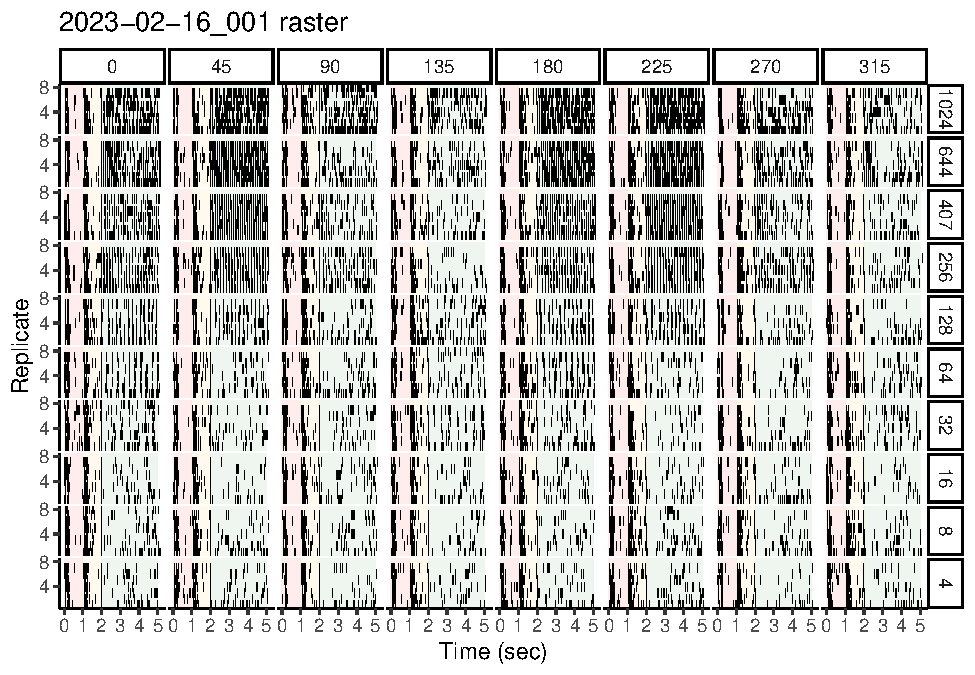
\includegraphics[width=800px,height=600px]{_main_files/figure-latex/rasterplot-1}

\hypertarget{mean-spike-rate-plots}{%
\section{Mean spike rate plots}\label{mean-spike-rate-plots}}

To visualize the mean spike rate over the course of the stimulus
sweep, I typically elect to use 100ms-binned data. This format of the
data allows me to see the salient spike rate patterns without focusing
on every little variation in the data.

Here, we will use \texttt{ggplot} to create a plot with:

\begin{enumerate}
\def\labelenumi{\arabic{enumi}.}
\tightlist
\item
  Data sub-plotted by stimulus (i.e., Speed and Direction)
\item
  Standardized sweep time on the x-axis, with delineation among
  blank, stationary, and moving phases
\item
  A black line to indicate the mean spike rate, along with a grey
  ribbon to show +/- 1 S.E.M.
\end{enumerate}

\begin{Shaded}
\begin{Highlighting}[]
\DocumentationTok{\#\# For each 100{-}ms binned file, generate a mean spike plot}
\NormalTok{bin100\_msr\_plots }\OtherTok{\textless{}{-}} \ConstantTok{NULL}
\ControlFlowTok{for}\NormalTok{ (i }\ControlFlowTok{in} \DecValTok{1}\SpecialCharTok{:}\FunctionTok{length}\NormalTok{(bin100\_filelist)) \{}
  \DocumentationTok{\#\# Read in the data}
\NormalTok{  bin100\_data }\OtherTok{\textless{}{-}}
    \FunctionTok{read\_csv}\NormalTok{(bin100\_filelist[i]) }\SpecialCharTok{\%\textgreater{}\%}
    \FunctionTok{as\_tibble}\NormalTok{()}

  \DocumentationTok{\#\# Compute SE and other metrics and add this to our data set}
\NormalTok{  dataslices\_100 }\OtherTok{\textless{}{-}}
\NormalTok{    bin100\_data }\SpecialCharTok{\%\textgreater{}\%}
    \DocumentationTok{\#\# Split by direction and speed, because we will use those to define each}
    \DocumentationTok{\#\# subplot}
    \FunctionTok{group\_split}\NormalTok{(Direction, Speed) }\SpecialCharTok{\%\textgreater{}\%}
    \DocumentationTok{\#\# Group by time bin}
\NormalTok{    purrr}\SpecialCharTok{::}\FunctionTok{map}\NormalTok{(group\_by, bin) }\SpecialCharTok{\%\textgreater{}\%}
    \DocumentationTok{\#\# Within each time bin, compute the following:}
\NormalTok{    purrr}\SpecialCharTok{::}\FunctionTok{map}\NormalTok{(transmute,}
               \DocumentationTok{\#\# first() can be used for metadata such as Speed or Direction}
               \AttributeTok{Speed =} \FunctionTok{first}\NormalTok{(Speed),}
               \AttributeTok{Direction =} \FunctionTok{first}\NormalTok{(Direction),}
               \DocumentationTok{\#\# I generally compute the mean within each bin for the following:}
               \AttributeTok{Time\_stand =} \FunctionTok{mean}\NormalTok{(Time\_stand),}
               \AttributeTok{Blank\_end =} \FunctionTok{mean}\NormalTok{(Blank\_end),}
               \AttributeTok{Static\_end =} \FunctionTok{mean}\NormalTok{(Static\_end),}
               \AttributeTok{Mean\_spike\_rate =} \FunctionTok{mean}\NormalTok{(Spike\_rate),}
               \DocumentationTok{\#\# To get SE, divide s.d. by the square root of sample size}
               \AttributeTok{Spike\_rate\_SE =} \FunctionTok{sd}\NormalTok{(Spike\_rate)}\SpecialCharTok{/}\FunctionTok{sqrt}\NormalTok{(}\FunctionTok{n}\NormalTok{()),}
               \AttributeTok{Mean\_photod\_rate =} \FunctionTok{mean}\NormalTok{(Photod\_mean),}
               \DocumentationTok{\#\# SE of photodiode}
               \AttributeTok{Photod\_SE =} \FunctionTok{sd}\NormalTok{(Photod\_mean)}\SpecialCharTok{/}\FunctionTok{sqrt}\NormalTok{(}\FunctionTok{n}\NormalTok{())}
\NormalTok{    ) }\SpecialCharTok{\%\textgreater{}\%}
\NormalTok{    purrr}\SpecialCharTok{::}\FunctionTok{map}\NormalTok{(ungroup) }\SpecialCharTok{\%\textgreater{}\%}
    \FunctionTok{bind\_rows}\NormalTok{() }\SpecialCharTok{\%\textgreater{}\%}
    \DocumentationTok{\#\# We\textquotesingle{}ll manually set the levels of the "Speed" column to ensure they plot in}
    \DocumentationTok{\#\# a desired order (fastest = highest, slowest = lowest)}
    \FunctionTok{mutate}\NormalTok{(}\FunctionTok{across}\NormalTok{(}
\NormalTok{      Speed,}
\NormalTok{      factor,}
      \AttributeTok{levels =} \FunctionTok{c}\NormalTok{(}\StringTok{"1024"}\NormalTok{, }\StringTok{"644"}\NormalTok{, }\StringTok{"407"}\NormalTok{, }\StringTok{"256"}\NormalTok{, }\StringTok{"128"}\NormalTok{, }\StringTok{"64"}\NormalTok{, }\StringTok{"32"}\NormalTok{, }\StringTok{"16"}\NormalTok{, }\StringTok{"8"}\NormalTok{, }\StringTok{"4"}\NormalTok{)}
\NormalTok{    ))}

  \DocumentationTok{\#\# Generate the mean spike rate plot using ggplot}
\NormalTok{  bin100\_msr\_plots[[i]] }\OtherTok{\textless{}{-}}
\NormalTok{    dataslices\_100 }\SpecialCharTok{\%\textgreater{}\%}
    \DocumentationTok{\#\# The same code block can be used to generate either the mean spike rate}
    \DocumentationTok{\#\# (shown below) or photodiode trace (commented out)}
    \FunctionTok{ggplot}\NormalTok{(}\FunctionTok{aes}\NormalTok{(}\AttributeTok{x =}\NormalTok{ Time\_stand,}
               \AttributeTok{y =}\NormalTok{ Mean\_spike\_rate }\CommentTok{\#Mean\_photod\_rate}
\NormalTok{    )) }\SpecialCharTok{+}
    \DocumentationTok{\#\# We\textquotesingle{}ll actually start by placing red, yellow, and green vertical lines to}
    \DocumentationTok{\#\# distinguish between blank, stationary, and moving phases}
    \DocumentationTok{\#\# This comes first so that it is the bottom{-}most layer and doesn\textquotesingle{}t obstruct}
    \DocumentationTok{\#\# the data}
    \FunctionTok{geom\_vline}\NormalTok{(}\AttributeTok{xintercept =} \DecValTok{0}\NormalTok{, }\AttributeTok{col =} \StringTok{"red"}\NormalTok{) }\SpecialCharTok{+}
    \FunctionTok{geom\_vline}\NormalTok{(}\AttributeTok{xintercept =} \FunctionTok{first}\NormalTok{(dataslices\_100}\SpecialCharTok{$}\NormalTok{Blank\_end),}
               \AttributeTok{col =} \StringTok{"darkgoldenrod1"}\NormalTok{) }\SpecialCharTok{+}
    \FunctionTok{geom\_vline}\NormalTok{(}\AttributeTok{xintercept =} \FunctionTok{first}\NormalTok{(dataslices\_100}\SpecialCharTok{$}\NormalTok{Static\_end),}
               \AttributeTok{col =} \StringTok{"forestgreen"}\NormalTok{) }\SpecialCharTok{+}
    \DocumentationTok{\#\# We\textquotesingle{}ll use \textasciigrave{}geom\_ribbon()\textasciigrave{} to shade in the SE traces}
    \FunctionTok{geom\_ribbon}\NormalTok{(}\FunctionTok{aes}\NormalTok{(}
      \AttributeTok{ymin =}\NormalTok{ Mean\_spike\_rate }\SpecialCharTok{{-}}\NormalTok{ Spike\_rate\_SE,}
      \AttributeTok{ymax =}\NormalTok{ Mean\_spike\_rate }\SpecialCharTok{+}\NormalTok{ Spike\_rate\_SE}
      \CommentTok{\# ymin = Mean\_photod\_rate {-} Photod\_SE,}
      \CommentTok{\# ymax = Mean\_photod\_rate + Photod\_SE}
\NormalTok{    ),}
    \AttributeTok{fill =} \StringTok{"grey80"}\NormalTok{) }\SpecialCharTok{+}
    \DocumentationTok{\#\# \textasciigrave{}geom\_line()\textasciigrave{} will be used to draw the mean spike rate itself on top of}
    \DocumentationTok{\#\# the SE traces}
    \FunctionTok{geom\_line}\NormalTok{(}\AttributeTok{linewidth =} \FloatTok{0.05}\NormalTok{) }\SpecialCharTok{+}
    \DocumentationTok{\#\# Add a title to help us know what cell this is}
    \FunctionTok{ggtitle}\NormalTok{(bin10\_basenames[}\DecValTok{1}\NormalTok{]) }\SpecialCharTok{+}
    \FunctionTok{xlab}\NormalTok{(}\StringTok{"Time (sec)"}\NormalTok{) }\SpecialCharTok{+}
    \FunctionTok{ylab}\NormalTok{(}\StringTok{"Spike rate (spikes/sec)"}\NormalTok{) }\SpecialCharTok{+}
    \DocumentationTok{\#\# To sub{-}plot by Speed and Direction, I typically use \textasciigrave{}facet\_grid()\textasciigrave{}. This}
    \DocumentationTok{\#\# method allows me to explicitly declare what the row{-} and column{-}wise}
    \DocumentationTok{\#\# grouping variables are}
    \FunctionTok{facet\_grid}\NormalTok{(}\AttributeTok{rows =} \FunctionTok{vars}\NormalTok{(Speed), }\AttributeTok{cols =} \FunctionTok{vars}\NormalTok{(Direction)) }\SpecialCharTok{+}
    \FunctionTok{theme\_classic}\NormalTok{()}

  \FunctionTok{rm}\NormalTok{(bin100\_data, dataslices\_100)}
\NormalTok{\}}
\end{Highlighting}
\end{Shaded}

\texttt{bin100\_msr\_plots} is now an object in the environment that contains one plot
per imported data file. To plot, simply call the index of the file you
wish to see. Since we only have 1 example file, we'll showcase the only
plot here:

\begin{Shaded}
\begin{Highlighting}[]
\DocumentationTok{\#\# Here\textquotesingle{}s the spike rate plot}
\NormalTok{bin100\_msr\_plots[[}\DecValTok{1}\NormalTok{]]}
\end{Highlighting}
\end{Shaded}

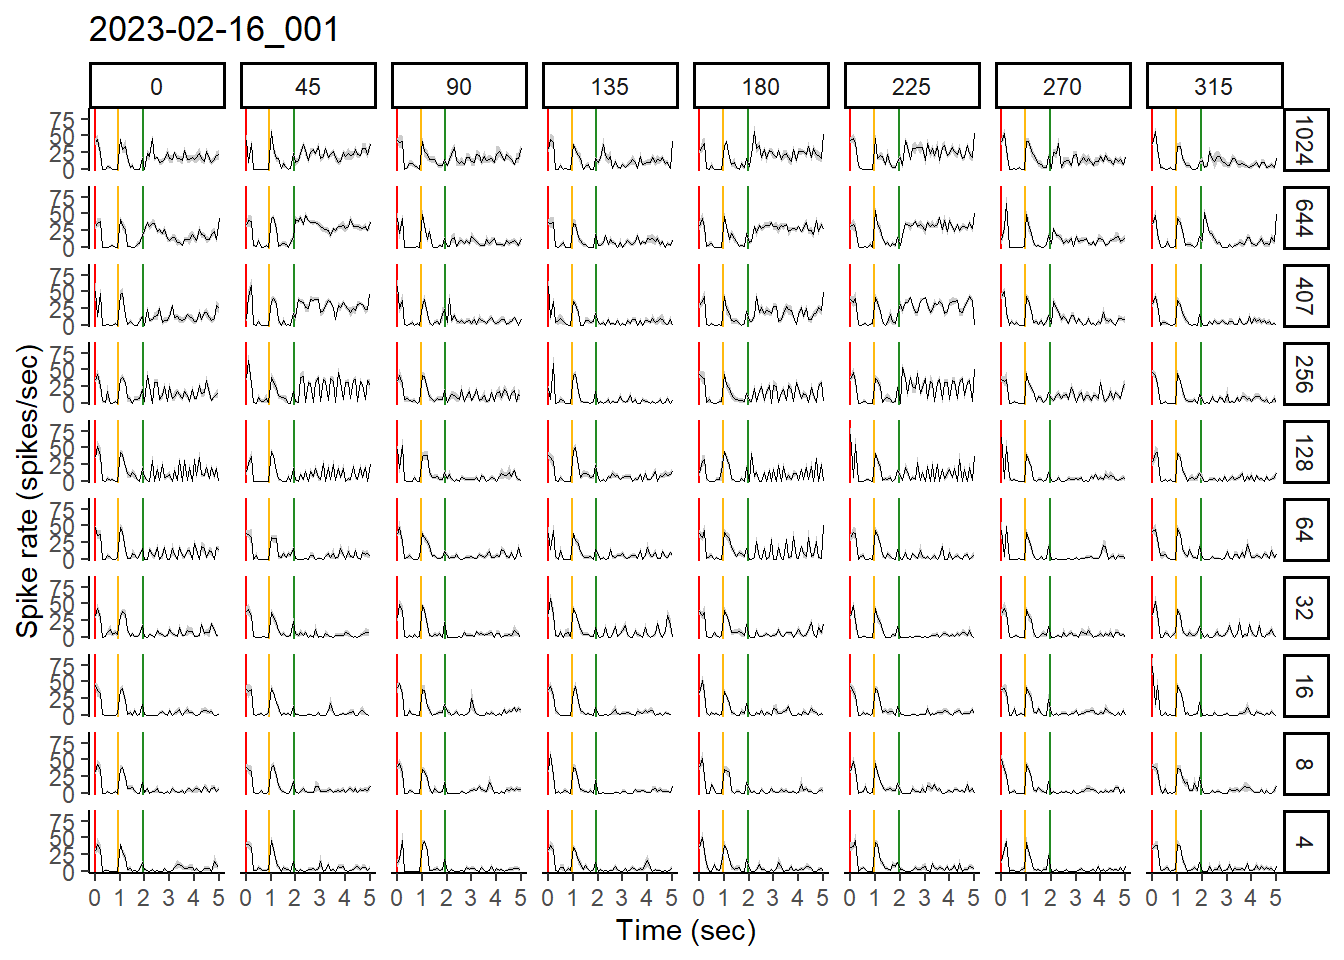
\includegraphics[width=800px,height=600px]{_main_files/figure-latex/msr_plot-1}

\hypertarget{export-to-pdf}{%
\section{Export to PDF}\label{export-to-pdf}}

Should you elect to either of these plots a \texttt{PDF}, here is an example
of what you could do.

\begin{Shaded}
\begin{Highlighting}[]
\DocumentationTok{\#\# Use the \textasciigrave{}pdf()\textasciigrave{} function to start the graphics device driver for producing}
\DocumentationTok{\#\# PDFs}
\DocumentationTok{\#\# Aspects such as page size and centering mode can be adjusted}
\FunctionTok{pdf}\NormalTok{(}
  \AttributeTok{file =} \StringTok{"./path/to/directory/2023{-}02{-}16\_001\_raster.pdf"}\NormalTok{,}
  \AttributeTok{width =} \FloatTok{10.5}\NormalTok{,}
  \AttributeTok{height =} \DecValTok{8}\NormalTok{,}
  \AttributeTok{title =} \StringTok{"2023{-}02{-}16\_001 raster"}\NormalTok{,}
  \AttributeTok{paper =} \StringTok{"USr"}\NormalTok{,}
  \AttributeTok{bg =} \StringTok{"white"}\NormalTok{,}
  \AttributeTok{pagecentre =} \ConstantTok{TRUE}\NormalTok{,}
  \AttributeTok{colormodel =} \StringTok{"srgb"}
\NormalTok{)}
\DocumentationTok{\#\# Now add the plot to the PDF simply by calling plot()}
\FunctionTok{plot}\NormalTok{(rasterplots[}\DecValTok{1}\NormalTok{])}
\DocumentationTok{\#\# To declare an end to this PDF writing session, use \textasciigrave{}dev.off()\textasciigrave{}}
\FunctionTok{dev.off}\NormalTok{()}
\end{Highlighting}
\end{Shaded}

\hypertarget{direction-tuning}{%
\chapter{Direction tuning}\label{direction-tuning}}

This type of plot is so fundamental to the examination of LM and nBOR,
it deserves a chapter unto itself. The majority of the information
going into polar tuning plots is the same as those in previous
chapters. Unlike raster and mean spike rate plots, however, direction
tuning plots require deliberate choices from the investigator to
delineate a ``baseline'' spike rate to be distinguished from the spike
rate during the stimulus of interest (in our case, global motion
patterns). The conditions that define the baseline and motion epochs
require explicit definitions form the investigator.

Seeing the mean spike rate plot from the previous chapter will help
give context to some of these decisions \textbf{{[}INSERT IMAGE HERE{]}}.
Importantly, at the onset of the blank and the stationary phases, it
is common to observe an initial transient response -- a sharp increase
in the spike rate of the neuron -- followed by a return to a steady
state.

For our purposes, the baseline will be defined as the steady state
response during the stationary phase of the stimulus. We will collect
this steady state response rate across all stimulus conditions (i.e.,
varying combos of speed and direction), and will simply average all of
those response rates to attain our baseline rate (and its SEM). Please
note that it is up to the investigator to determine if this definition
is appropriate, especially if other stimulus presentations are being
used.

For the ``motion epoch'', I will use a few different definitions. Some
of these conventions are informed by previous work (e.g., Smyth et al.
2022), whereas others are just based on a rough approximation of what
may be appropriate for these data. The definitions of the motion
epochs will be:

\begin{enumerate}
\def\labelenumi{\arabic{enumi}.}
\tightlist
\item
  The entire 3-sec motion epoch
\item
  The ``initial transient'' phase: 40-200ms after the onset of
  motion (as used in Smyth et al.~2022)
\item
  The ``steady state'' phase: 1500-3000ms after the onset of motion,
  a.k.a., the second half of the motion stimulus (as used in Smyth
  et al.~2022)
\item
  The first 500 ms of the motion phase. This is an arbitrary
  definition for demonstrative purposes only, but somewhat informed
  by observing the patterns in the mean spike rate plot
\end{enumerate}

As we construct polar plots, two additional aspects will be included
in the plots:

\begin{enumerate}
\def\labelenumi{\arabic{enumi}.}
\tightlist
\item
  The ``preferred direction'' of the neuron, as defined by the vector
  sum method \textbf{{[}insert citation{]}}. This will be shown as a single
  grey line in the plot that indicates the preferred direction. Bear
  in mind that this value may not always be meaningful, particularly
  in cases of multi-modal responses.
\item
  The Sensitivity Index (SI) of the neuron, as defined by
  \textbf{\protect\hyperlink{citation}{citation}}. This metric calculates the narrowness of tuning.
  An SI of 1 indicates strong response to a single direction whereas
  0 indicates similar response across all investigated directions.
\end{enumerate}

\hypertarget{data-import-and-baseline-rate-measurement}{%
\section{Data import and baseline rate measurement}\label{data-import-and-baseline-rate-measurement}}

We will use the 10-ms binned data for these examples. We'll read in the
file and then extract the baseline rate as defined above.

\begin{Shaded}
\begin{Highlighting}[]
\DocumentationTok{\#\# Read in the data}
\DocumentationTok{\#\# Since there is only 1 example file, we\textquotesingle{}ll simplify things by just}
\DocumentationTok{\#\# subsetting bin10\_filelist}
\NormalTok{bin10\_data }\OtherTok{\textless{}{-}}
  \FunctionTok{read\_csv}\NormalTok{(bin10\_filelist[}\DecValTok{1}\NormalTok{], }\AttributeTok{show\_col\_types =} \ConstantTok{FALSE}\NormalTok{) }\SpecialCharTok{\%\textgreater{}\%}
  \FunctionTok{as\_tibble}\NormalTok{() }\SpecialCharTok{\%\textgreater{}\%}
  \DocumentationTok{\#\# Again, we will set Speed as an ordered factor to help control plotting}
  \DocumentationTok{\#\# later on}
  \FunctionTok{mutate}\NormalTok{(}\FunctionTok{across}\NormalTok{(}
\NormalTok{    Speed,}
\NormalTok{    factor,}
    \AttributeTok{levels =} \FunctionTok{c}\NormalTok{(}\StringTok{"1024"}\NormalTok{, }\StringTok{"644"}\NormalTok{, }\StringTok{"407"}\NormalTok{, }\StringTok{"256"}\NormalTok{, }\StringTok{"128"}\NormalTok{, }\StringTok{"64"}\NormalTok{, }\StringTok{"32"}\NormalTok{, }\StringTok{"16"}\NormalTok{, }\StringTok{"8"}\NormalTok{, }\StringTok{"4"}\NormalTok{)}
\NormalTok{  ))}

\DocumentationTok{\#\# Extract all rows corresponding to our desired baseline epoch}
\NormalTok{baseline\_df }\OtherTok{\textless{}{-}}
\NormalTok{  bin10\_data }\SpecialCharTok{\%\textgreater{}\%}
  \FunctionTok{filter}\NormalTok{(Time\_stand }\SpecialCharTok{\textgreater{}=}\NormalTok{ Blank\_end }\SpecialCharTok{+} \FloatTok{0.5}\NormalTok{) }\SpecialCharTok{\%\textgreater{}\%} \DocumentationTok{\#\# 0.5 sec after blank end}
  \FunctionTok{filter}\NormalTok{(Time\_stand }\SpecialCharTok{\textless{}=}\NormalTok{ Static\_end }\SpecialCharTok{{-}} \FloatTok{0.05}\NormalTok{)   }\DocumentationTok{\#\# 0.05 sec before static end}

\DocumentationTok{\#\# Compute the mean baseline}
\NormalTok{global\_base }\OtherTok{\textless{}{-}} \FunctionTok{mean}\NormalTok{(baseline\_df}\SpecialCharTok{$}\NormalTok{Spike\_rate)}
\DocumentationTok{\#\# Compute the SE}
\NormalTok{global\_base\_se }\OtherTok{\textless{}{-}}
  \FunctionTok{sd}\NormalTok{(baseline\_df}\SpecialCharTok{$}\NormalTok{Spike\_rate) }\SpecialCharTok{/} \FunctionTok{sqrt}\NormalTok{(}\FunctionTok{length}\NormalTok{(baseline\_df}\SpecialCharTok{$}\NormalTok{Spike\_rate)}\CommentTok{\#/45}
\NormalTok{  )}

\DocumentationTok{\#\# Construct a summary data frame}
\NormalTok{baseline\_summary\_df }\OtherTok{\textless{}{-}}
\NormalTok{  baseline\_df }\SpecialCharTok{\%\textgreater{}\%}
  \FunctionTok{group\_by}\NormalTok{(Speed) }\SpecialCharTok{\%\textgreater{}\%}
  \FunctionTok{summarize}\NormalTok{(}
    \AttributeTok{speed\_specific\_baseline =} \FunctionTok{mean}\NormalTok{(Spike\_rate),}
    \AttributeTok{speed\_specific\_baseline\_se =} \FunctionTok{sd}\NormalTok{(Spike\_rate)}\SpecialCharTok{/}\FunctionTok{sqrt}\NormalTok{(}\FunctionTok{length}\NormalTok{(Spike\_rate)),}
    \AttributeTok{global\_baseline =}\NormalTok{ global\_base,}
    \AttributeTok{global\_baseline\_se =}\NormalTok{ global\_base\_se}
\NormalTok{  )}

\DocumentationTok{\#\# This tibble contains speed{-}specific baselines (and SE) along with the global}
\DocumentationTok{\#\# mean baseline (and SE)}
\NormalTok{baseline\_summary\_df}
\end{Highlighting}
\end{Shaded}

\begin{verbatim}
## # A tibble: 10 x 5
##    Speed speed_specific_baseline speed_specific_baseline_se global_bas~1 globa~2
##    <fct>                   <dbl>                      <dbl>        <dbl>   <dbl>
##  1 1024                     4.44                      0.516         3.81   0.153
##  2 644                      2.99                      0.441         3.81   0.153
##  3 407                      4.18                      0.534         3.81   0.153
##  4 256                      4.41                      0.521         3.81   0.153
##  5 128                      4.58                      0.529         3.81   0.153
##  6 64                       4.45                      0.523         3.81   0.153
##  7 32                       3.57                      0.468         3.81   0.153
##  8 16                       2.55                      0.390         3.81   0.153
##  9 8                        3.86                      0.469         3.81   0.153
## 10 4                        3.04                      0.425         3.81   0.153
## # ... with abbreviated variable names 1: global_baseline, 2: global_baseline_se
\end{verbatim}

\hypertarget{using-the-full-3-sec-motion-epoch}{%
\section{Using the full 3-sec motion epoch}\label{using-the-full-3-sec-motion-epoch}}

This will be referred to as the ``naive'' approach in the code below

\begin{Shaded}
\begin{Highlighting}[]
\DocumentationTok{\#\# global baseline values, full 3{-}sec motion period}
\NormalTok{naive\_df }\OtherTok{\textless{}{-}}
\NormalTok{  bin10\_data }\SpecialCharTok{\%\textgreater{}\%}
  \FunctionTok{filter}\NormalTok{(Time\_stand }\SpecialCharTok{\textgreater{}}\NormalTok{ Static\_end) }\SpecialCharTok{\%\textgreater{}\%}
  \FunctionTok{group\_by}\NormalTok{(Speed, Direction, Replicate) }\SpecialCharTok{\%\textgreater{}\%}
  \FunctionTok{summarize}\NormalTok{(}
    \AttributeTok{mean\_spike\_rate =} \FunctionTok{mean}\NormalTok{(Spike\_rate)}
\NormalTok{  )}
\end{Highlighting}
\end{Shaded}

\begin{verbatim}
## `summarise()` has grouped output by 'Speed', 'Direction'. You can override
## using the `.groups` argument.
\end{verbatim}

\begin{Shaded}
\begin{Highlighting}[]
\NormalTok{naive\_360 }\OtherTok{\textless{}{-}}
\NormalTok{  naive\_df }\SpecialCharTok{\%\textgreater{}\%}
  \FunctionTok{filter}\NormalTok{(Direction }\SpecialCharTok{==} \DecValTok{0}\NormalTok{) }\SpecialCharTok{\%\textgreater{}\%}
  \FunctionTok{transmute}\NormalTok{(}
    \AttributeTok{Speed =}\NormalTok{ Speed,}
    \AttributeTok{Direction =} \DecValTok{360}\NormalTok{,}
    \AttributeTok{Replicate =}\NormalTok{ Replicate,}
    \AttributeTok{mean\_spike\_rate =}\NormalTok{ mean\_spike\_rate)}
\NormalTok{naive\_vecsum\_df }\OtherTok{\textless{}{-}}
\NormalTok{  naive\_df }\SpecialCharTok{\%\textgreater{}\%}
  \FunctionTok{ungroup}\NormalTok{() }\SpecialCharTok{\%\textgreater{}\%}
  \FunctionTok{drop\_na}\NormalTok{(mean\_spike\_rate) }\SpecialCharTok{\%\textgreater{}\%}
  \FunctionTok{group\_split}\NormalTok{(Speed) }\SpecialCharTok{\%\textgreater{}\%}
  \FunctionTok{map}\NormalTok{(group\_by, Direction) }\SpecialCharTok{\%\textgreater{}\%}
  \DocumentationTok{\#\# }\AlertTok{NOTE}\DocumentationTok{: FOLLOWING THE JNP AND CB PAPERS, WE ARE SUBTRACTING BASELINE HERE AND}
  \DocumentationTok{\#\# THEN IF ANY AVERAGED FIRING RATES ARE NEGATIVE, THEY ARE SHIFTED SO THE}
  \DocumentationTok{\#\# LOWEST ONE IS ZERO. THE GENERATED PLOTS STILL SHOW NON{-}BASELINE{-}SUBTRACTED}
  \DocumentationTok{\#\# FIRING RATES (AND BASELINE AS A RED RING), BUT COMPUTATION OF VECTOR SUM}
  \DocumentationTok{\#\# AND SI HAVE BEEN BASELINE SUBTRACTED (AND THE ENTIRE CURVE IS SHIFTED}
  \DocumentationTok{\#\# UPWARDS IF ANY PART IS NEGATIVE)}
  \FunctionTok{map}\NormalTok{(summarize,}
      \AttributeTok{mean\_spike\_rate =} \FunctionTok{mean}\NormalTok{(mean\_spike\_rate) }\SpecialCharTok{{-}}\NormalTok{ global\_base,}
      \AttributeTok{Speed =} \FunctionTok{first}\NormalTok{(Speed)) }\SpecialCharTok{\%\textgreater{}\%}
  \FunctionTok{map}\NormalTok{(mutate,}
      \AttributeTok{mean\_spike\_rate =}
        \FunctionTok{case\_when}\NormalTok{(}\FunctionTok{min}\NormalTok{(mean\_spike\_rate) }\SpecialCharTok{\textless{}} \DecValTok{0} \SpecialCharTok{\textasciitilde{}}\NormalTok{ mean\_spike\_rate }\SpecialCharTok{+} \FunctionTok{abs}\NormalTok{(}\FunctionTok{min}\NormalTok{(mean\_spike\_rate)),}
                  \ConstantTok{TRUE} \SpecialCharTok{\textasciitilde{}}\NormalTok{ mean\_spike\_rate)) }\SpecialCharTok{\%\textgreater{}\%}
  \FunctionTok{map}\NormalTok{(transmute,}
      \AttributeTok{x =} \FunctionTok{cos}\NormalTok{(Direction }\SpecialCharTok{*}\NormalTok{ pi }\SpecialCharTok{/} \DecValTok{180}\NormalTok{) }\SpecialCharTok{*}\NormalTok{ mean\_spike\_rate,}
      \AttributeTok{y =} \FunctionTok{sin}\NormalTok{(Direction }\SpecialCharTok{*}\NormalTok{ pi }\SpecialCharTok{/} \DecValTok{180}\NormalTok{) }\SpecialCharTok{*}\NormalTok{ mean\_spike\_rate,}
      \AttributeTok{Speed =} \FunctionTok{first}\NormalTok{(Speed)}
\NormalTok{  ) }\SpecialCharTok{\%\textgreater{}\%}
  \FunctionTok{map}\NormalTok{(summarise,}
      \AttributeTok{x =} \FunctionTok{mean}\NormalTok{(x),}
      \AttributeTok{y =} \FunctionTok{mean}\NormalTok{(y),}
      \AttributeTok{Speed =} \FunctionTok{first}\NormalTok{(Speed)) }\SpecialCharTok{\%\textgreater{}\%}
  \FunctionTok{map}\NormalTok{(transmute,}
      \AttributeTok{vector\_sum =}\NormalTok{ (}\FunctionTok{atan2}\NormalTok{(y, x) }\SpecialCharTok{*} \DecValTok{180} \SpecialCharTok{/}\NormalTok{ pi) }\SpecialCharTok{\%\%} \DecValTok{360}\NormalTok{,}
      \AttributeTok{Speed =} \FunctionTok{first}\NormalTok{(Speed)}
\NormalTok{  ) }\SpecialCharTok{\%\textgreater{}\%}
  \FunctionTok{bind\_rows}\NormalTok{()}
\NormalTok{naive\_si\_df}\OtherTok{\textless{}{-}}
\NormalTok{  naive\_df }\SpecialCharTok{\%\textgreater{}\%}
  \FunctionTok{ungroup}\NormalTok{() }\SpecialCharTok{\%\textgreater{}\%}
  \FunctionTok{drop\_na}\NormalTok{(mean\_spike\_rate) }\SpecialCharTok{\%\textgreater{}\%}
  \FunctionTok{group\_split}\NormalTok{(Speed) }\SpecialCharTok{\%\textgreater{}\%}
  \FunctionTok{map}\NormalTok{(group\_by, Direction) }\SpecialCharTok{\%\textgreater{}\%}
  \FunctionTok{map}\NormalTok{(summarize,}
      \AttributeTok{mean\_spike\_rate =} \FunctionTok{mean}\NormalTok{(mean\_spike\_rate) }\SpecialCharTok{{-}}\NormalTok{ global\_base,}
      \AttributeTok{Speed =} \FunctionTok{first}\NormalTok{(Speed)) }\SpecialCharTok{\%\textgreater{}\%}
  \FunctionTok{map}\NormalTok{(mutate,}
      \AttributeTok{mean\_spike\_rate =}
        \FunctionTok{case\_when}\NormalTok{(}\FunctionTok{min}\NormalTok{(mean\_spike\_rate) }\SpecialCharTok{\textless{}} \DecValTok{0} \SpecialCharTok{\textasciitilde{}}\NormalTok{ mean\_spike\_rate }\SpecialCharTok{+} \FunctionTok{abs}\NormalTok{(}\FunctionTok{min}\NormalTok{(mean\_spike\_rate)),}
                  \ConstantTok{TRUE} \SpecialCharTok{\textasciitilde{}}\NormalTok{ mean\_spike\_rate)) }\SpecialCharTok{\%\textgreater{}\%}
  \FunctionTok{map}\NormalTok{(transmute,}
      \AttributeTok{a =}\NormalTok{ (}\FunctionTok{sin}\NormalTok{(Direction }\SpecialCharTok{*}\NormalTok{ pi }\SpecialCharTok{/} \DecValTok{180}\NormalTok{) }\SpecialCharTok{*}\NormalTok{ mean\_spike\_rate),}
      \AttributeTok{b =}\NormalTok{ (}\FunctionTok{cos}\NormalTok{(Direction }\SpecialCharTok{*}\NormalTok{ pi }\SpecialCharTok{/} \DecValTok{180}\NormalTok{) }\SpecialCharTok{*}\NormalTok{ mean\_spike\_rate),}
      \AttributeTok{c =} \FunctionTok{mean}\NormalTok{(mean\_spike\_rate),}
      \AttributeTok{Speed =} \FunctionTok{first}\NormalTok{(Speed)}
\NormalTok{  ) }\SpecialCharTok{\%\textgreater{}\%}
  \FunctionTok{map}\NormalTok{(summarise,}
      \AttributeTok{a =} \FunctionTok{mean}\NormalTok{(a),}
      \AttributeTok{b =} \FunctionTok{mean}\NormalTok{(b),}
      \AttributeTok{c =} \FunctionTok{mean}\NormalTok{(c),}
      \AttributeTok{Speed =} \FunctionTok{first}\NormalTok{(Speed)) }\SpecialCharTok{\%\textgreater{}\%}
  \FunctionTok{map}\NormalTok{(transmute,}
      \AttributeTok{si =} \FunctionTok{sqrt}\NormalTok{(a }\SpecialCharTok{\^{}} \DecValTok{2} \SpecialCharTok{+}\NormalTok{ b }\SpecialCharTok{\^{}} \DecValTok{2}\NormalTok{) }\SpecialCharTok{/}\NormalTok{ c,}
      \AttributeTok{Speed =} \FunctionTok{first}\NormalTok{(Speed)}
\NormalTok{  ) }\SpecialCharTok{\%\textgreater{}\%}
  \FunctionTok{bind\_rows}\NormalTok{()}

\NormalTok{naive\_data }\OtherTok{\textless{}{-}}
\NormalTok{  naive\_df }\SpecialCharTok{\%\textgreater{}\%}
  \FunctionTok{bind\_rows}\NormalTok{(naive\_360) }\SpecialCharTok{\%\textgreater{}\%}
  \FunctionTok{left\_join}\NormalTok{(naive\_vecsum\_df, }\AttributeTok{by =} \StringTok{"Speed"}\NormalTok{) }\SpecialCharTok{\%\textgreater{}\%}
  \FunctionTok{left\_join}\NormalTok{(naive\_si\_df, }\AttributeTok{by =} \StringTok{"Speed"}\NormalTok{) }\SpecialCharTok{\%\textgreater{}\%}
  \FunctionTok{drop\_na}\NormalTok{(mean\_spike\_rate)}
\NormalTok{naive\_max\_y }\OtherTok{\textless{}{-}} \FunctionTok{max}\NormalTok{(naive\_data}\SpecialCharTok{$}\NormalTok{mean\_spike\_rate)}

\NormalTok{naive }\OtherTok{\textless{}{-}}
\NormalTok{  naive\_data }\SpecialCharTok{\%\textgreater{}\%}
  \FunctionTok{left\_join}\NormalTok{(baseline\_summary\_df, }\AttributeTok{by =} \StringTok{"Speed"}\NormalTok{) }\SpecialCharTok{\%\textgreater{}\%}
  \FunctionTok{ggplot}\NormalTok{(}\FunctionTok{aes}\NormalTok{(}\AttributeTok{x =}\NormalTok{ Direction, }\AttributeTok{y =}\NormalTok{ mean\_spike\_rate)) }\SpecialCharTok{+}
  \FunctionTok{geom\_ribbon}\NormalTok{(}\FunctionTok{aes}\NormalTok{(}
    \AttributeTok{x =}\NormalTok{ Direction,}
    \AttributeTok{ymin =}\NormalTok{ global\_baseline }\SpecialCharTok{{-}}\NormalTok{ global\_baseline\_se,}
    \AttributeTok{ymax =}\NormalTok{ global\_baseline }\SpecialCharTok{+}\NormalTok{ global\_baseline\_se}
\NormalTok{  ),}
  \AttributeTok{fill =} \StringTok{"red"}\NormalTok{) }\SpecialCharTok{+}
  \FunctionTok{stat\_smooth}\NormalTok{(}\AttributeTok{method =} \StringTok{"glm"}\NormalTok{, }\AttributeTok{formula =}\NormalTok{ y }\SpecialCharTok{\textasciitilde{}} \FunctionTok{ns}\NormalTok{(x,}\DecValTok{8}\NormalTok{), }\AttributeTok{size =} \FloatTok{0.3}\NormalTok{) }\SpecialCharTok{+}
  \FunctionTok{geom\_point}\NormalTok{() }\SpecialCharTok{+}
  \FunctionTok{geom\_label}\NormalTok{(}\FunctionTok{aes}\NormalTok{(}\AttributeTok{label =} \FunctionTok{round}\NormalTok{(si, }\DecValTok{2}\NormalTok{) , }\AttributeTok{x =} \DecValTok{315}\NormalTok{, }\AttributeTok{y =}\NormalTok{ naive\_max\_y }\SpecialCharTok{*} \FloatTok{1.2}\NormalTok{),}
             \AttributeTok{size =} \DecValTok{3}\NormalTok{) }\SpecialCharTok{+}
  \FunctionTok{geom\_vline}\NormalTok{(}\FunctionTok{aes}\NormalTok{(}\AttributeTok{xintercept =}\NormalTok{ vector\_sum), }\AttributeTok{colour =} \StringTok{"grey30"}\NormalTok{,}
             \AttributeTok{size =} \FloatTok{0.75}\NormalTok{) }\SpecialCharTok{+}
  \FunctionTok{coord\_polar}\NormalTok{(}\AttributeTok{direction =} \DecValTok{1}\NormalTok{, }\AttributeTok{start =}\NormalTok{ pi}\SpecialCharTok{/}\DecValTok{2}\NormalTok{) }\SpecialCharTok{+}
  \FunctionTok{scale\_x\_continuous}\NormalTok{(}
    \AttributeTok{breaks =} \FunctionTok{c}\NormalTok{(}\DecValTok{0}\NormalTok{, }\DecValTok{90}\NormalTok{, }\DecValTok{180}\NormalTok{, }\DecValTok{270}\NormalTok{),}
    \AttributeTok{expand =} \FunctionTok{c}\NormalTok{(}\DecValTok{0}\NormalTok{, }\DecValTok{0}\NormalTok{),}
    \AttributeTok{limits =} \FunctionTok{c}\NormalTok{(}\DecValTok{0}\NormalTok{, }\DecValTok{360}\NormalTok{)}
\NormalTok{  )}\SpecialCharTok{+}
  \FunctionTok{facet\_grid}\NormalTok{(}\AttributeTok{rows =} \FunctionTok{vars}\NormalTok{(Speed)) }\SpecialCharTok{+}
  \FunctionTok{ggtitle}\NormalTok{(}\StringTok{"full 3{-}sec motion"}\NormalTok{) }\SpecialCharTok{+}
  \FunctionTok{theme\_minimal}\NormalTok{()}
\end{Highlighting}
\end{Shaded}

\begin{verbatim}
## Warning: Using `size` aesthetic for lines was deprecated in ggplot2 3.4.0.
## i Please use `linewidth` instead.
\end{verbatim}

\begin{Shaded}
\begin{Highlighting}[]
\NormalTok{naive}
\end{Highlighting}
\end{Shaded}

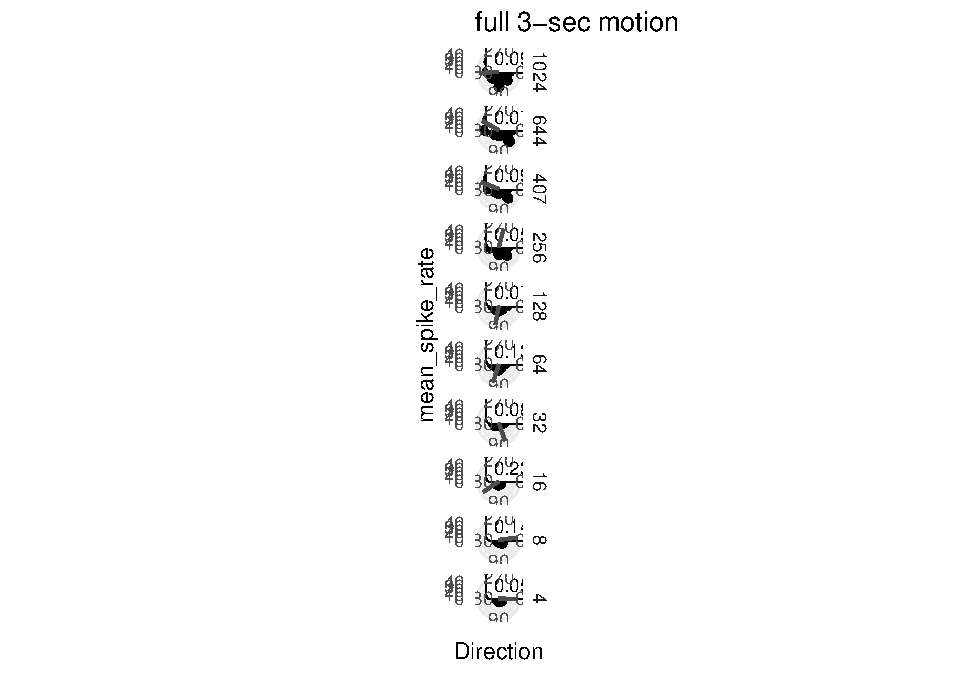
\includegraphics{_main_files/figure-latex/naive-1.pdf}

\hypertarget{using-40-200ms-initial-transient}{%
\section{Using 40-200ms (``initial transient'')}\label{using-40-200ms-initial-transient}}

\begin{Shaded}
\begin{Highlighting}[]
\DocumentationTok{\#\# global baseline values, 40{-}200 msec motion period}
\NormalTok{cbit\_df }\OtherTok{\textless{}{-}}
\NormalTok{  bin10\_data }\SpecialCharTok{\%\textgreater{}\%}
  \FunctionTok{filter}\NormalTok{(Time\_stand }\SpecialCharTok{\textgreater{}=}\NormalTok{ Static\_end }\SpecialCharTok{+} \FloatTok{0.04}\NormalTok{) }\SpecialCharTok{\%\textgreater{}\%}
  \FunctionTok{filter}\NormalTok{(Time\_stand }\SpecialCharTok{\textless{}=}\NormalTok{ Static\_end }\SpecialCharTok{+} \FloatTok{0.2}\NormalTok{) }\SpecialCharTok{\%\textgreater{}\%}
  \FunctionTok{group\_by}\NormalTok{(Speed, Direction, Replicate) }\SpecialCharTok{\%\textgreater{}\%}
  \FunctionTok{summarize}\NormalTok{(}
    \AttributeTok{mean\_spike\_rate =} \FunctionTok{mean}\NormalTok{(Spike\_rate)}
\NormalTok{  )}
\end{Highlighting}
\end{Shaded}

\begin{verbatim}
## `summarise()` has grouped output by 'Speed', 'Direction'. You can override
## using the `.groups` argument.
\end{verbatim}

\begin{Shaded}
\begin{Highlighting}[]
\NormalTok{cbit\_360 }\OtherTok{\textless{}{-}}
\NormalTok{  cbit\_df }\SpecialCharTok{\%\textgreater{}\%}
  \FunctionTok{filter}\NormalTok{(Direction }\SpecialCharTok{==} \DecValTok{0}\NormalTok{) }\SpecialCharTok{\%\textgreater{}\%}
  \FunctionTok{transmute}\NormalTok{(}
    \AttributeTok{Speed =}\NormalTok{ Speed,}
    \AttributeTok{Direction =} \DecValTok{360}\NormalTok{,}
    \AttributeTok{Replicate =}\NormalTok{ Replicate,}
    \AttributeTok{mean\_spike\_rate =}\NormalTok{ mean\_spike\_rate)}
\NormalTok{cbit\_vecsum\_df }\OtherTok{\textless{}{-}}
\NormalTok{  cbit\_df }\SpecialCharTok{\%\textgreater{}\%}
  \FunctionTok{ungroup}\NormalTok{() }\SpecialCharTok{\%\textgreater{}\%}
  \FunctionTok{drop\_na}\NormalTok{(mean\_spike\_rate) }\SpecialCharTok{\%\textgreater{}\%}
  \FunctionTok{group\_split}\NormalTok{(Speed) }\SpecialCharTok{\%\textgreater{}\%}
  \FunctionTok{map}\NormalTok{(group\_by, Direction) }\SpecialCharTok{\%\textgreater{}\%}
  \FunctionTok{map}\NormalTok{(summarize,}
      \AttributeTok{mean\_spike\_rate =} \FunctionTok{mean}\NormalTok{(mean\_spike\_rate) }\SpecialCharTok{{-}}\NormalTok{ global\_base,}
      \AttributeTok{Speed =} \FunctionTok{first}\NormalTok{(Speed)) }\SpecialCharTok{\%\textgreater{}\%}
  \FunctionTok{map}\NormalTok{(mutate,}
      \AttributeTok{mean\_spike\_rate =}
        \FunctionTok{case\_when}\NormalTok{(}\FunctionTok{min}\NormalTok{(mean\_spike\_rate) }\SpecialCharTok{\textless{}} \DecValTok{0} \SpecialCharTok{\textasciitilde{}}\NormalTok{ mean\_spike\_rate }\SpecialCharTok{+} \FunctionTok{abs}\NormalTok{(}\FunctionTok{min}\NormalTok{(mean\_spike\_rate)),}
                  \ConstantTok{TRUE} \SpecialCharTok{\textasciitilde{}}\NormalTok{ mean\_spike\_rate)) }\SpecialCharTok{\%\textgreater{}\%}
  \FunctionTok{map}\NormalTok{(transmute,}
      \AttributeTok{x =} \FunctionTok{cos}\NormalTok{(Direction }\SpecialCharTok{*}\NormalTok{ pi }\SpecialCharTok{/} \DecValTok{180}\NormalTok{) }\SpecialCharTok{*}\NormalTok{ mean\_spike\_rate,}
      \AttributeTok{y =} \FunctionTok{sin}\NormalTok{(Direction }\SpecialCharTok{*}\NormalTok{ pi }\SpecialCharTok{/} \DecValTok{180}\NormalTok{) }\SpecialCharTok{*}\NormalTok{ mean\_spike\_rate,}
      \AttributeTok{Speed =} \FunctionTok{first}\NormalTok{(Speed)}
\NormalTok{  ) }\SpecialCharTok{\%\textgreater{}\%}
  \FunctionTok{map}\NormalTok{(summarise,}
      \AttributeTok{x =} \FunctionTok{mean}\NormalTok{(x),}
      \AttributeTok{y =} \FunctionTok{mean}\NormalTok{(y),}
      \AttributeTok{Speed =} \FunctionTok{first}\NormalTok{(Speed)) }\SpecialCharTok{\%\textgreater{}\%}
  \FunctionTok{map}\NormalTok{(transmute,}
      \AttributeTok{vector\_sum =}\NormalTok{ (}\FunctionTok{atan2}\NormalTok{(y, x) }\SpecialCharTok{*} \DecValTok{180} \SpecialCharTok{/}\NormalTok{ pi) }\SpecialCharTok{\%\%} \DecValTok{360}\NormalTok{,}
      \AttributeTok{Speed =} \FunctionTok{first}\NormalTok{(Speed)}
\NormalTok{  ) }\SpecialCharTok{\%\textgreater{}\%}
  \FunctionTok{bind\_rows}\NormalTok{()}
\NormalTok{cbit\_si\_df }\OtherTok{\textless{}{-}}
\NormalTok{  cbit\_df }\SpecialCharTok{\%\textgreater{}\%}
  \FunctionTok{ungroup}\NormalTok{() }\SpecialCharTok{\%\textgreater{}\%}
  \FunctionTok{drop\_na}\NormalTok{(mean\_spike\_rate) }\SpecialCharTok{\%\textgreater{}\%}
  \FunctionTok{group\_split}\NormalTok{(Speed) }\SpecialCharTok{\%\textgreater{}\%}
  \FunctionTok{map}\NormalTok{(group\_by, Direction) }\SpecialCharTok{\%\textgreater{}\%}
  \FunctionTok{map}\NormalTok{(summarize,}
      \AttributeTok{mean\_spike\_rate =} \FunctionTok{mean}\NormalTok{(mean\_spike\_rate) }\SpecialCharTok{{-}}\NormalTok{ global\_base,}
      \AttributeTok{Speed =} \FunctionTok{first}\NormalTok{(Speed)) }\SpecialCharTok{\%\textgreater{}\%}
  \FunctionTok{map}\NormalTok{(mutate,}
      \AttributeTok{mean\_spike\_rate =}
        \FunctionTok{case\_when}\NormalTok{(}\FunctionTok{min}\NormalTok{(mean\_spike\_rate) }\SpecialCharTok{\textless{}} \DecValTok{0} \SpecialCharTok{\textasciitilde{}}\NormalTok{ mean\_spike\_rate }\SpecialCharTok{+} \FunctionTok{abs}\NormalTok{(}\FunctionTok{min}\NormalTok{(mean\_spike\_rate)),}
                  \ConstantTok{TRUE} \SpecialCharTok{\textasciitilde{}}\NormalTok{ mean\_spike\_rate)) }\SpecialCharTok{\%\textgreater{}\%}
  \FunctionTok{map}\NormalTok{(transmute,}
      \AttributeTok{a =}\NormalTok{ (}\FunctionTok{sin}\NormalTok{(Direction }\SpecialCharTok{*}\NormalTok{ pi }\SpecialCharTok{/} \DecValTok{180}\NormalTok{) }\SpecialCharTok{*}\NormalTok{ mean\_spike\_rate),}
      \AttributeTok{b =}\NormalTok{ (}\FunctionTok{cos}\NormalTok{(Direction }\SpecialCharTok{*}\NormalTok{ pi }\SpecialCharTok{/} \DecValTok{180}\NormalTok{) }\SpecialCharTok{*}\NormalTok{ mean\_spike\_rate),}
      \AttributeTok{c =} \FunctionTok{mean}\NormalTok{(mean\_spike\_rate),}
      \AttributeTok{Speed =} \FunctionTok{first}\NormalTok{(Speed)}
\NormalTok{  ) }\SpecialCharTok{\%\textgreater{}\%}
  \FunctionTok{map}\NormalTok{(summarise,}
      \AttributeTok{a =} \FunctionTok{mean}\NormalTok{(a),}
      \AttributeTok{b =} \FunctionTok{mean}\NormalTok{(b),}
      \AttributeTok{c =} \FunctionTok{mean}\NormalTok{(c),}
      \AttributeTok{Speed =} \FunctionTok{first}\NormalTok{(Speed)) }\SpecialCharTok{\%\textgreater{}\%}
  \FunctionTok{map}\NormalTok{(transmute,}
      \AttributeTok{si =} \FunctionTok{sqrt}\NormalTok{(a }\SpecialCharTok{\^{}} \DecValTok{2} \SpecialCharTok{+}\NormalTok{ b }\SpecialCharTok{\^{}} \DecValTok{2}\NormalTok{) }\SpecialCharTok{/}\NormalTok{ c,}
      \AttributeTok{Speed =} \FunctionTok{first}\NormalTok{(Speed)}
\NormalTok{  ) }\SpecialCharTok{\%\textgreater{}\%}
  \FunctionTok{bind\_rows}\NormalTok{()}

\NormalTok{cbit\_data }\OtherTok{\textless{}{-}}
\NormalTok{  cbit\_df }\SpecialCharTok{\%\textgreater{}\%}
  \FunctionTok{bind\_rows}\NormalTok{(cbit\_360) }\SpecialCharTok{\%\textgreater{}\%}
  \FunctionTok{left\_join}\NormalTok{(cbit\_vecsum\_df, }\AttributeTok{by =} \StringTok{"Speed"}\NormalTok{) }\SpecialCharTok{\%\textgreater{}\%}
  \FunctionTok{left\_join}\NormalTok{(cbit\_si\_df, }\AttributeTok{by =} \StringTok{"Speed"}\NormalTok{) }\SpecialCharTok{\%\textgreater{}\%}
  \FunctionTok{drop\_na}\NormalTok{(mean\_spike\_rate)}
\NormalTok{cbit\_max\_y }\OtherTok{\textless{}{-}} \FunctionTok{max}\NormalTok{(cbit\_data}\SpecialCharTok{$}\NormalTok{mean\_spike\_rate)}

\NormalTok{cb\_it }\OtherTok{\textless{}{-}}
\NormalTok{  cbit\_data }\SpecialCharTok{\%\textgreater{}\%}
  \FunctionTok{left\_join}\NormalTok{(baseline\_summary\_df, }\AttributeTok{by =} \StringTok{"Speed"}\NormalTok{) }\SpecialCharTok{\%\textgreater{}\%}
  \FunctionTok{ggplot}\NormalTok{(}\FunctionTok{aes}\NormalTok{(}\AttributeTok{x =}\NormalTok{ Direction, }\AttributeTok{y =}\NormalTok{ mean\_spike\_rate)) }\SpecialCharTok{+}
  \FunctionTok{geom\_ribbon}\NormalTok{(}\FunctionTok{aes}\NormalTok{(}
    \AttributeTok{x =}\NormalTok{ Direction,}
    \AttributeTok{ymin =}\NormalTok{ global\_baseline }\SpecialCharTok{{-}}\NormalTok{ global\_baseline\_se,}
    \AttributeTok{ymax =}\NormalTok{ global\_baseline }\SpecialCharTok{+}\NormalTok{ global\_baseline\_se}
\NormalTok{  ),}
  \AttributeTok{fill =} \StringTok{"red"}\NormalTok{) }\SpecialCharTok{+}
  \FunctionTok{stat\_smooth}\NormalTok{(}\AttributeTok{method =} \StringTok{"glm"}\NormalTok{, }\AttributeTok{formula =}\NormalTok{ y }\SpecialCharTok{\textasciitilde{}} \FunctionTok{ns}\NormalTok{(x,}\DecValTok{8}\NormalTok{), }\AttributeTok{size =} \FloatTok{0.3}\NormalTok{) }\SpecialCharTok{+}
  \FunctionTok{geom\_point}\NormalTok{() }\SpecialCharTok{+}
  \FunctionTok{geom\_label}\NormalTok{(}\FunctionTok{aes}\NormalTok{(}\AttributeTok{label =} \FunctionTok{round}\NormalTok{(si, }\DecValTok{2}\NormalTok{) , }\AttributeTok{x =} \DecValTok{315}\NormalTok{, }\AttributeTok{y =}\NormalTok{ cbit\_max\_y }\SpecialCharTok{*} \FloatTok{1.2}\NormalTok{),}
             \AttributeTok{size =} \DecValTok{3}\NormalTok{) }\SpecialCharTok{+}
  \FunctionTok{geom\_vline}\NormalTok{(}\FunctionTok{aes}\NormalTok{(}\AttributeTok{xintercept =}\NormalTok{ vector\_sum), }\AttributeTok{colour =} \StringTok{"grey30"}\NormalTok{,}
             \AttributeTok{size =} \FloatTok{0.75}\NormalTok{) }\SpecialCharTok{+}
  \FunctionTok{coord\_polar}\NormalTok{(}\AttributeTok{direction =} \DecValTok{1}\NormalTok{, }\AttributeTok{start =}\NormalTok{ pi}\SpecialCharTok{/}\DecValTok{2}\NormalTok{) }\SpecialCharTok{+}
  \FunctionTok{scale\_x\_continuous}\NormalTok{(}
    \AttributeTok{breaks =} \FunctionTok{c}\NormalTok{(}\DecValTok{0}\NormalTok{, }\DecValTok{90}\NormalTok{, }\DecValTok{180}\NormalTok{, }\DecValTok{270}\NormalTok{),}
    \AttributeTok{expand =} \FunctionTok{c}\NormalTok{(}\DecValTok{0}\NormalTok{, }\DecValTok{0}\NormalTok{),}
    \AttributeTok{limits =} \FunctionTok{c}\NormalTok{(}\DecValTok{0}\NormalTok{, }\DecValTok{360}\NormalTok{)}
\NormalTok{  )}\SpecialCharTok{+}
  \FunctionTok{facet\_grid}\NormalTok{(}\AttributeTok{rows =} \FunctionTok{vars}\NormalTok{(Speed)) }\SpecialCharTok{+}
  \FunctionTok{ggtitle}\NormalTok{(}\StringTok{"40{-}200 msec motion"}\NormalTok{) }\SpecialCharTok{+}
  \FunctionTok{theme\_minimal}\NormalTok{()}

\NormalTok{cb\_it}
\end{Highlighting}
\end{Shaded}

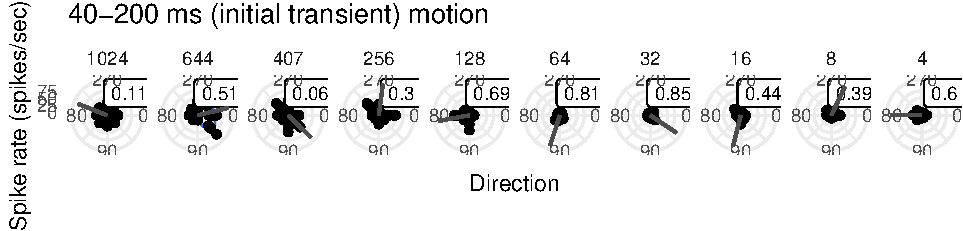
\includegraphics{_main_files/figure-latex/cb_it-1.pdf}

\hypertarget{using-1500-3000ms-steady-state}{%
\section{Using 1500-3000ms (``steady state'')}\label{using-1500-3000ms-steady-state}}

\begin{Shaded}
\begin{Highlighting}[]
\DocumentationTok{\#\# global baseline values, second half of motion period}
\NormalTok{cbss\_df }\OtherTok{\textless{}{-}}
\NormalTok{  bin10\_data }\SpecialCharTok{\%\textgreater{}\%}
  \FunctionTok{filter}\NormalTok{(Time\_stand }\SpecialCharTok{\textgreater{}}\NormalTok{ Static\_end }\SpecialCharTok{+} \FloatTok{1.5}\NormalTok{) }\SpecialCharTok{\%\textgreater{}\%}
  \FunctionTok{filter}\NormalTok{(Time\_stand }\SpecialCharTok{\textless{}} \FloatTok{4.95}\NormalTok{) }\SpecialCharTok{\%\textgreater{}\%}
  \FunctionTok{group\_by}\NormalTok{(Speed, Direction, Replicate) }\SpecialCharTok{\%\textgreater{}\%}
  \FunctionTok{summarize}\NormalTok{(}
    \AttributeTok{mean\_spike\_rate =} \FunctionTok{mean}\NormalTok{(Spike\_rate)}
\NormalTok{  )}
\end{Highlighting}
\end{Shaded}

\begin{verbatim}
## `summarise()` has grouped output by 'Speed', 'Direction'. You can override
## using the `.groups` argument.
\end{verbatim}

\begin{Shaded}
\begin{Highlighting}[]
\NormalTok{cbss\_360 }\OtherTok{\textless{}{-}}
\NormalTok{  cbss\_df }\SpecialCharTok{\%\textgreater{}\%}
  \FunctionTok{filter}\NormalTok{(Direction }\SpecialCharTok{==} \DecValTok{0}\NormalTok{) }\SpecialCharTok{\%\textgreater{}\%}
  \FunctionTok{transmute}\NormalTok{(}
    \AttributeTok{Speed =}\NormalTok{ Speed,}
    \AttributeTok{Direction =} \DecValTok{360}\NormalTok{,}
    \AttributeTok{Replicate =}\NormalTok{ Replicate,}
    \AttributeTok{mean\_spike\_rate =}\NormalTok{ mean\_spike\_rate)}
\NormalTok{cbss\_vecsum\_df }\OtherTok{\textless{}{-}}
\NormalTok{  cbss\_df }\SpecialCharTok{\%\textgreater{}\%}
  \FunctionTok{ungroup}\NormalTok{() }\SpecialCharTok{\%\textgreater{}\%}
  \FunctionTok{drop\_na}\NormalTok{(mean\_spike\_rate) }\SpecialCharTok{\%\textgreater{}\%}
  \FunctionTok{group\_split}\NormalTok{(Speed) }\SpecialCharTok{\%\textgreater{}\%}
  \FunctionTok{map}\NormalTok{(group\_by, Direction) }\SpecialCharTok{\%\textgreater{}\%}
  \FunctionTok{map}\NormalTok{(summarize,}
      \AttributeTok{mean\_spike\_rate =} \FunctionTok{mean}\NormalTok{(mean\_spike\_rate) }\SpecialCharTok{{-}}\NormalTok{ global\_base,}
      \AttributeTok{Speed =} \FunctionTok{first}\NormalTok{(Speed)) }\SpecialCharTok{\%\textgreater{}\%}
  \FunctionTok{map}\NormalTok{(mutate,}
      \AttributeTok{mean\_spike\_rate =}
        \FunctionTok{case\_when}\NormalTok{(}\FunctionTok{min}\NormalTok{(mean\_spike\_rate) }\SpecialCharTok{\textless{}} \DecValTok{0} \SpecialCharTok{\textasciitilde{}}\NormalTok{ mean\_spike\_rate }\SpecialCharTok{+} \FunctionTok{abs}\NormalTok{(}\FunctionTok{min}\NormalTok{(mean\_spike\_rate)),}
                  \ConstantTok{TRUE} \SpecialCharTok{\textasciitilde{}}\NormalTok{ mean\_spike\_rate)) }\SpecialCharTok{\%\textgreater{}\%}
  \FunctionTok{map}\NormalTok{(transmute,}
      \AttributeTok{x =} \FunctionTok{cos}\NormalTok{(Direction }\SpecialCharTok{*}\NormalTok{ pi }\SpecialCharTok{/} \DecValTok{180}\NormalTok{) }\SpecialCharTok{*}\NormalTok{ mean\_spike\_rate,}
      \AttributeTok{y =} \FunctionTok{sin}\NormalTok{(Direction }\SpecialCharTok{*}\NormalTok{ pi }\SpecialCharTok{/} \DecValTok{180}\NormalTok{) }\SpecialCharTok{*}\NormalTok{ mean\_spike\_rate,}
      \AttributeTok{Speed =} \FunctionTok{first}\NormalTok{(Speed)}
\NormalTok{  ) }\SpecialCharTok{\%\textgreater{}\%}
  \FunctionTok{map}\NormalTok{(summarise,}
      \AttributeTok{x =} \FunctionTok{mean}\NormalTok{(x),}
      \AttributeTok{y =} \FunctionTok{mean}\NormalTok{(y),}
      \AttributeTok{Speed =} \FunctionTok{first}\NormalTok{(Speed)) }\SpecialCharTok{\%\textgreater{}\%}
  \FunctionTok{map}\NormalTok{(transmute,}
      \AttributeTok{vector\_sum =}\NormalTok{ (}\FunctionTok{atan2}\NormalTok{(y, x) }\SpecialCharTok{*} \DecValTok{180} \SpecialCharTok{/}\NormalTok{ pi) }\SpecialCharTok{\%\%} \DecValTok{360}\NormalTok{,}
      \AttributeTok{Speed =} \FunctionTok{first}\NormalTok{(Speed)}
\NormalTok{  ) }\SpecialCharTok{\%\textgreater{}\%}
  \FunctionTok{bind\_rows}\NormalTok{()}
\NormalTok{cbss\_si\_df }\OtherTok{\textless{}{-}}
\NormalTok{  cbss\_df }\SpecialCharTok{\%\textgreater{}\%}
  \FunctionTok{ungroup}\NormalTok{() }\SpecialCharTok{\%\textgreater{}\%}
  \FunctionTok{drop\_na}\NormalTok{(mean\_spike\_rate) }\SpecialCharTok{\%\textgreater{}\%}
  \FunctionTok{group\_split}\NormalTok{(Speed) }\SpecialCharTok{\%\textgreater{}\%}
  \FunctionTok{map}\NormalTok{(group\_by, Direction) }\SpecialCharTok{\%\textgreater{}\%}
  \FunctionTok{map}\NormalTok{(summarize,}
      \AttributeTok{mean\_spike\_rate =} \FunctionTok{mean}\NormalTok{(mean\_spike\_rate) }\SpecialCharTok{{-}}\NormalTok{ global\_base,}
      \AttributeTok{Speed =} \FunctionTok{first}\NormalTok{(Speed)) }\SpecialCharTok{\%\textgreater{}\%}
  \FunctionTok{map}\NormalTok{(mutate,}
      \AttributeTok{mean\_spike\_rate =}
        \FunctionTok{case\_when}\NormalTok{(}\FunctionTok{min}\NormalTok{(mean\_spike\_rate) }\SpecialCharTok{\textless{}} \DecValTok{0} \SpecialCharTok{\textasciitilde{}}\NormalTok{ mean\_spike\_rate }\SpecialCharTok{+} \FunctionTok{abs}\NormalTok{(}\FunctionTok{min}\NormalTok{(mean\_spike\_rate)),}
                  \ConstantTok{TRUE} \SpecialCharTok{\textasciitilde{}}\NormalTok{ mean\_spike\_rate)) }\SpecialCharTok{\%\textgreater{}\%}
  \FunctionTok{map}\NormalTok{(transmute,}
      \AttributeTok{a =}\NormalTok{ (}\FunctionTok{sin}\NormalTok{(Direction }\SpecialCharTok{*}\NormalTok{ pi }\SpecialCharTok{/} \DecValTok{180}\NormalTok{) }\SpecialCharTok{*}\NormalTok{ mean\_spike\_rate),}
      \AttributeTok{b =}\NormalTok{ (}\FunctionTok{cos}\NormalTok{(Direction }\SpecialCharTok{*}\NormalTok{ pi }\SpecialCharTok{/} \DecValTok{180}\NormalTok{) }\SpecialCharTok{*}\NormalTok{ mean\_spike\_rate),}
      \AttributeTok{c =} \FunctionTok{mean}\NormalTok{(mean\_spike\_rate),}
      \AttributeTok{Speed =} \FunctionTok{first}\NormalTok{(Speed)}
\NormalTok{  ) }\SpecialCharTok{\%\textgreater{}\%}
  \FunctionTok{map}\NormalTok{(summarise,}
      \AttributeTok{a =} \FunctionTok{mean}\NormalTok{(a),}
      \AttributeTok{b =} \FunctionTok{mean}\NormalTok{(b),}
      \AttributeTok{c =} \FunctionTok{mean}\NormalTok{(c),}
      \AttributeTok{Speed =} \FunctionTok{first}\NormalTok{(Speed)) }\SpecialCharTok{\%\textgreater{}\%}
  \FunctionTok{map}\NormalTok{(transmute,}
      \AttributeTok{si =} \FunctionTok{sqrt}\NormalTok{(a }\SpecialCharTok{\^{}} \DecValTok{2} \SpecialCharTok{+}\NormalTok{ b }\SpecialCharTok{\^{}} \DecValTok{2}\NormalTok{) }\SpecialCharTok{/}\NormalTok{ c,}
      \AttributeTok{Speed =} \FunctionTok{first}\NormalTok{(Speed)}
\NormalTok{  ) }\SpecialCharTok{\%\textgreater{}\%}
  \FunctionTok{bind\_rows}\NormalTok{()}

\NormalTok{cbss\_data }\OtherTok{\textless{}{-}}
\NormalTok{  cbss\_df }\SpecialCharTok{\%\textgreater{}\%}
  \FunctionTok{bind\_rows}\NormalTok{(cbss\_360) }\SpecialCharTok{\%\textgreater{}\%}
  \FunctionTok{left\_join}\NormalTok{(cbss\_vecsum\_df, }\AttributeTok{by =} \StringTok{"Speed"}\NormalTok{) }\SpecialCharTok{\%\textgreater{}\%}
  \FunctionTok{left\_join}\NormalTok{(cbss\_si\_df, }\AttributeTok{by =} \StringTok{"Speed"}\NormalTok{) }\SpecialCharTok{\%\textgreater{}\%}
  \FunctionTok{drop\_na}\NormalTok{(mean\_spike\_rate)}
\NormalTok{cbss\_max\_y }\OtherTok{\textless{}{-}} \FunctionTok{max}\NormalTok{(cbss\_data}\SpecialCharTok{$}\NormalTok{mean\_spike\_rate)}


\NormalTok{cb\_ss }\OtherTok{\textless{}{-}}
\NormalTok{  cbss\_data }\SpecialCharTok{\%\textgreater{}\%}
  \FunctionTok{left\_join}\NormalTok{(baseline\_summary\_df, }\AttributeTok{by =} \StringTok{"Speed"}\NormalTok{) }\SpecialCharTok{\%\textgreater{}\%}
  \FunctionTok{ggplot}\NormalTok{(}\FunctionTok{aes}\NormalTok{(}\AttributeTok{x =}\NormalTok{ Direction, }\AttributeTok{y =}\NormalTok{ mean\_spike\_rate)) }\SpecialCharTok{+}
  \FunctionTok{geom\_ribbon}\NormalTok{(}\FunctionTok{aes}\NormalTok{(}
    \AttributeTok{x =}\NormalTok{ Direction,}
    \AttributeTok{ymin =}\NormalTok{ global\_baseline }\SpecialCharTok{{-}}\NormalTok{ global\_baseline\_se,}
    \AttributeTok{ymax =}\NormalTok{ global\_baseline }\SpecialCharTok{+}\NormalTok{ global\_baseline\_se}
\NormalTok{  ),}
  \AttributeTok{fill =} \StringTok{"red"}\NormalTok{) }\SpecialCharTok{+}
  \FunctionTok{stat\_smooth}\NormalTok{(}\AttributeTok{method =} \StringTok{"glm"}\NormalTok{, }\AttributeTok{formula =}\NormalTok{ y }\SpecialCharTok{\textasciitilde{}} \FunctionTok{ns}\NormalTok{(x,}\DecValTok{8}\NormalTok{), }\AttributeTok{size =} \FloatTok{0.3}\NormalTok{) }\SpecialCharTok{+}
  \FunctionTok{geom\_point}\NormalTok{() }\SpecialCharTok{+}
  \FunctionTok{geom\_label}\NormalTok{(}\FunctionTok{aes}\NormalTok{(}\AttributeTok{label =} \FunctionTok{round}\NormalTok{(si, }\DecValTok{2}\NormalTok{) , }\AttributeTok{x =} \DecValTok{315}\NormalTok{, }\AttributeTok{y =}\NormalTok{ cbss\_max\_y }\SpecialCharTok{*} \FloatTok{1.2}\NormalTok{),}
             \AttributeTok{size =} \DecValTok{3}\NormalTok{) }\SpecialCharTok{+}
  \FunctionTok{geom\_vline}\NormalTok{(}\FunctionTok{aes}\NormalTok{(}\AttributeTok{xintercept =}\NormalTok{ vector\_sum), }\AttributeTok{colour =} \StringTok{"grey30"}\NormalTok{,}
             \AttributeTok{size =} \FloatTok{0.75}\NormalTok{) }\SpecialCharTok{+}
  \FunctionTok{coord\_polar}\NormalTok{(}\AttributeTok{direction =} \DecValTok{1}\NormalTok{, }\AttributeTok{start =}\NormalTok{ pi}\SpecialCharTok{/}\DecValTok{2}\NormalTok{) }\SpecialCharTok{+}
  \FunctionTok{scale\_x\_continuous}\NormalTok{(}
    \AttributeTok{breaks =} \FunctionTok{c}\NormalTok{(}\DecValTok{0}\NormalTok{, }\DecValTok{90}\NormalTok{, }\DecValTok{180}\NormalTok{, }\DecValTok{270}\NormalTok{),}
    \AttributeTok{expand =} \FunctionTok{c}\NormalTok{(}\DecValTok{0}\NormalTok{, }\DecValTok{0}\NormalTok{),}
    \AttributeTok{limits =} \FunctionTok{c}\NormalTok{(}\DecValTok{0}\NormalTok{, }\DecValTok{360}\NormalTok{)}
\NormalTok{  )}\SpecialCharTok{+}
  \FunctionTok{facet\_grid}\NormalTok{(}\AttributeTok{rows =} \FunctionTok{vars}\NormalTok{(Speed)) }\SpecialCharTok{+}
  \FunctionTok{ggtitle}\NormalTok{(}\StringTok{"steady state motion"}\NormalTok{) }\SpecialCharTok{+}
  \FunctionTok{theme\_minimal}\NormalTok{()}

\NormalTok{cb\_ss}
\end{Highlighting}
\end{Shaded}

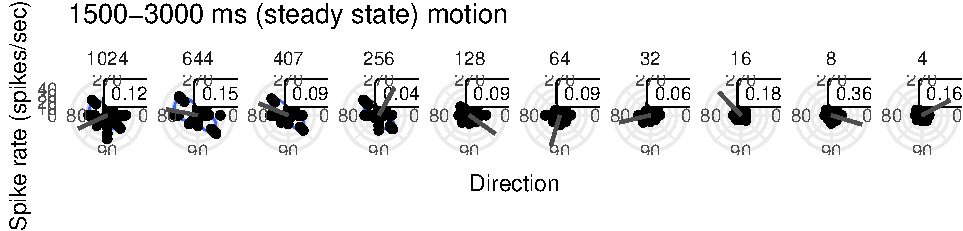
\includegraphics{_main_files/figure-latex/cb_ss-1.pdf}

\hypertarget{using-0-500-ms-arbitrary-epoch-length}{%
\section{Using 0-500 ms (arbitrary epoch length)}\label{using-0-500-ms-arbitrary-epoch-length}}

\begin{Shaded}
\begin{Highlighting}[]
\DocumentationTok{\#\# global baseline values, 0{-}500 msec motion period}
\NormalTok{arb\_df }\OtherTok{\textless{}{-}}
\NormalTok{  bin10\_data }\SpecialCharTok{\%\textgreater{}\%}
  \FunctionTok{filter}\NormalTok{(Time\_stand }\SpecialCharTok{\textgreater{}=}\NormalTok{ Static\_end }\SpecialCharTok{+} \FloatTok{0.001}\NormalTok{) }\SpecialCharTok{\%\textgreater{}\%}
  \FunctionTok{filter}\NormalTok{(Time\_stand }\SpecialCharTok{\textless{}=}\NormalTok{ Static\_end }\SpecialCharTok{+} \FloatTok{0.500}\NormalTok{) }\SpecialCharTok{\%\textgreater{}\%}
  \FunctionTok{group\_by}\NormalTok{(Speed, Direction, Replicate) }\SpecialCharTok{\%\textgreater{}\%}
  \FunctionTok{summarize}\NormalTok{(}
    \AttributeTok{mean\_spike\_rate =} \FunctionTok{mean}\NormalTok{(Spike\_rate)}
\NormalTok{  )}
\end{Highlighting}
\end{Shaded}

\begin{verbatim}
## `summarise()` has grouped output by 'Speed', 'Direction'. You can override
## using the `.groups` argument.
\end{verbatim}

\begin{Shaded}
\begin{Highlighting}[]
\NormalTok{arb\_360 }\OtherTok{\textless{}{-}}
\NormalTok{  arb\_df }\SpecialCharTok{\%\textgreater{}\%}
  \FunctionTok{filter}\NormalTok{(Direction }\SpecialCharTok{==} \DecValTok{0}\NormalTok{) }\SpecialCharTok{\%\textgreater{}\%}
  \FunctionTok{transmute}\NormalTok{(}
    \AttributeTok{Speed =}\NormalTok{ Speed,}
    \AttributeTok{Direction =} \DecValTok{360}\NormalTok{,}
    \AttributeTok{Replicate =}\NormalTok{ Replicate,}
    \AttributeTok{mean\_spike\_rate =}\NormalTok{ mean\_spike\_rate)}
\NormalTok{arb\_vecsum\_df }\OtherTok{\textless{}{-}}
\NormalTok{  arb\_df }\SpecialCharTok{\%\textgreater{}\%}
  \FunctionTok{ungroup}\NormalTok{() }\SpecialCharTok{\%\textgreater{}\%}
  \FunctionTok{drop\_na}\NormalTok{(mean\_spike\_rate) }\SpecialCharTok{\%\textgreater{}\%}
  \FunctionTok{group\_split}\NormalTok{(Speed) }\SpecialCharTok{\%\textgreater{}\%}
  \FunctionTok{map}\NormalTok{(group\_by, Direction) }\SpecialCharTok{\%\textgreater{}\%}
  \FunctionTok{map}\NormalTok{(summarize,}
      \AttributeTok{mean\_spike\_rate =} \FunctionTok{mean}\NormalTok{(mean\_spike\_rate) }\SpecialCharTok{{-}}\NormalTok{ global\_base,}
      \AttributeTok{Speed =} \FunctionTok{first}\NormalTok{(Speed)) }\SpecialCharTok{\%\textgreater{}\%}
  \FunctionTok{map}\NormalTok{(mutate,}
      \AttributeTok{mean\_spike\_rate =}
        \FunctionTok{case\_when}\NormalTok{(}\FunctionTok{min}\NormalTok{(mean\_spike\_rate) }\SpecialCharTok{\textless{}} \DecValTok{0} \SpecialCharTok{\textasciitilde{}}\NormalTok{ mean\_spike\_rate }\SpecialCharTok{+} \FunctionTok{abs}\NormalTok{(}\FunctionTok{min}\NormalTok{(mean\_spike\_rate)),}
                  \ConstantTok{TRUE} \SpecialCharTok{\textasciitilde{}}\NormalTok{ mean\_spike\_rate)) }\SpecialCharTok{\%\textgreater{}\%}
  \FunctionTok{map}\NormalTok{(transmute,}
      \AttributeTok{x =} \FunctionTok{cos}\NormalTok{(Direction }\SpecialCharTok{*}\NormalTok{ pi }\SpecialCharTok{/} \DecValTok{180}\NormalTok{) }\SpecialCharTok{*}\NormalTok{ mean\_spike\_rate,}
      \AttributeTok{y =} \FunctionTok{sin}\NormalTok{(Direction }\SpecialCharTok{*}\NormalTok{ pi }\SpecialCharTok{/} \DecValTok{180}\NormalTok{) }\SpecialCharTok{*}\NormalTok{ mean\_spike\_rate,}
      \AttributeTok{Speed =} \FunctionTok{first}\NormalTok{(Speed)}
\NormalTok{  ) }\SpecialCharTok{\%\textgreater{}\%}
  \FunctionTok{map}\NormalTok{(summarise,}
      \AttributeTok{x =} \FunctionTok{mean}\NormalTok{(x),}
      \AttributeTok{y =} \FunctionTok{mean}\NormalTok{(y),}
      \AttributeTok{Speed =} \FunctionTok{first}\NormalTok{(Speed)) }\SpecialCharTok{\%\textgreater{}\%}
  \FunctionTok{map}\NormalTok{(transmute,}
      \AttributeTok{vector\_sum =}\NormalTok{ (}\FunctionTok{atan2}\NormalTok{(y, x) }\SpecialCharTok{*} \DecValTok{180} \SpecialCharTok{/}\NormalTok{ pi) }\SpecialCharTok{\%\%} \DecValTok{360}\NormalTok{,}
      \AttributeTok{Speed =} \FunctionTok{first}\NormalTok{(Speed)}
\NormalTok{  ) }\SpecialCharTok{\%\textgreater{}\%}
  \FunctionTok{bind\_rows}\NormalTok{()}
\NormalTok{arb\_si\_df }\OtherTok{\textless{}{-}}
\NormalTok{  arb\_df }\SpecialCharTok{\%\textgreater{}\%}
  \FunctionTok{ungroup}\NormalTok{() }\SpecialCharTok{\%\textgreater{}\%}
  \FunctionTok{drop\_na}\NormalTok{(mean\_spike\_rate) }\SpecialCharTok{\%\textgreater{}\%}
  \FunctionTok{group\_split}\NormalTok{(Speed) }\SpecialCharTok{\%\textgreater{}\%}
  \FunctionTok{map}\NormalTok{(group\_by, Direction) }\SpecialCharTok{\%\textgreater{}\%}
  \FunctionTok{map}\NormalTok{(summarize,}
      \AttributeTok{mean\_spike\_rate =} \FunctionTok{mean}\NormalTok{(mean\_spike\_rate) }\SpecialCharTok{{-}}\NormalTok{ global\_base,}
      \AttributeTok{Speed =} \FunctionTok{first}\NormalTok{(Speed)) }\SpecialCharTok{\%\textgreater{}\%}
  \FunctionTok{map}\NormalTok{(mutate,}
      \AttributeTok{mean\_spike\_rate =}
        \FunctionTok{case\_when}\NormalTok{(}\FunctionTok{min}\NormalTok{(mean\_spike\_rate) }\SpecialCharTok{\textless{}} \DecValTok{0} \SpecialCharTok{\textasciitilde{}}\NormalTok{ mean\_spike\_rate }\SpecialCharTok{+} \FunctionTok{abs}\NormalTok{(}\FunctionTok{min}\NormalTok{(mean\_spike\_rate)),}
                  \ConstantTok{TRUE} \SpecialCharTok{\textasciitilde{}}\NormalTok{ mean\_spike\_rate)) }\SpecialCharTok{\%\textgreater{}\%}
  \FunctionTok{map}\NormalTok{(transmute,}
      \AttributeTok{a =}\NormalTok{ (}\FunctionTok{sin}\NormalTok{(Direction }\SpecialCharTok{*}\NormalTok{ pi }\SpecialCharTok{/} \DecValTok{180}\NormalTok{) }\SpecialCharTok{*}\NormalTok{ mean\_spike\_rate),}
      \AttributeTok{b =}\NormalTok{ (}\FunctionTok{cos}\NormalTok{(Direction }\SpecialCharTok{*}\NormalTok{ pi }\SpecialCharTok{/} \DecValTok{180}\NormalTok{) }\SpecialCharTok{*}\NormalTok{ mean\_spike\_rate),}
      \AttributeTok{c =} \FunctionTok{mean}\NormalTok{(mean\_spike\_rate),}
      \AttributeTok{Speed =} \FunctionTok{first}\NormalTok{(Speed)}
\NormalTok{  ) }\SpecialCharTok{\%\textgreater{}\%}
  \FunctionTok{map}\NormalTok{(summarise,}
      \AttributeTok{a =} \FunctionTok{mean}\NormalTok{(a),}
      \AttributeTok{b =} \FunctionTok{mean}\NormalTok{(b),}
      \AttributeTok{c =} \FunctionTok{mean}\NormalTok{(c),}
      \AttributeTok{Speed =} \FunctionTok{first}\NormalTok{(Speed)) }\SpecialCharTok{\%\textgreater{}\%}
  \FunctionTok{map}\NormalTok{(transmute,}
      \AttributeTok{si =} \FunctionTok{sqrt}\NormalTok{(a }\SpecialCharTok{\^{}} \DecValTok{2} \SpecialCharTok{+}\NormalTok{ b }\SpecialCharTok{\^{}} \DecValTok{2}\NormalTok{) }\SpecialCharTok{/}\NormalTok{ c,}
      \AttributeTok{Speed =} \FunctionTok{first}\NormalTok{(Speed)}
\NormalTok{  ) }\SpecialCharTok{\%\textgreater{}\%}
  \FunctionTok{bind\_rows}\NormalTok{()}

\NormalTok{arb\_data }\OtherTok{\textless{}{-}}
\NormalTok{  arb\_df }\SpecialCharTok{\%\textgreater{}\%}
  \FunctionTok{bind\_rows}\NormalTok{(arb\_360) }\SpecialCharTok{\%\textgreater{}\%}
  \FunctionTok{left\_join}\NormalTok{(arb\_vecsum\_df, }\AttributeTok{by =} \StringTok{"Speed"}\NormalTok{) }\SpecialCharTok{\%\textgreater{}\%}
  \FunctionTok{left\_join}\NormalTok{(arb\_si\_df, }\AttributeTok{by =} \StringTok{"Speed"}\NormalTok{) }\SpecialCharTok{\%\textgreater{}\%}
  \FunctionTok{drop\_na}\NormalTok{(mean\_spike\_rate)}
\NormalTok{arb\_max\_y }\OtherTok{\textless{}{-}} \FunctionTok{max}\NormalTok{(arb\_data}\SpecialCharTok{$}\NormalTok{mean\_spike\_rate)}

\NormalTok{arb }\OtherTok{\textless{}{-}}
\NormalTok{  arb\_data }\SpecialCharTok{\%\textgreater{}\%}
  \FunctionTok{left\_join}\NormalTok{(baseline\_summary\_df, }\AttributeTok{by =} \StringTok{"Speed"}\NormalTok{) }\SpecialCharTok{\%\textgreater{}\%}
  \FunctionTok{ggplot}\NormalTok{(}\FunctionTok{aes}\NormalTok{(}\AttributeTok{x =}\NormalTok{ Direction, }\AttributeTok{y =}\NormalTok{ mean\_spike\_rate)) }\SpecialCharTok{+}
  \FunctionTok{geom\_ribbon}\NormalTok{(}\FunctionTok{aes}\NormalTok{(}
    \AttributeTok{x =}\NormalTok{ Direction,}
    \AttributeTok{ymin =}\NormalTok{ global\_baseline }\SpecialCharTok{{-}}\NormalTok{ global\_baseline\_se,}
    \AttributeTok{ymax =}\NormalTok{ global\_baseline }\SpecialCharTok{+}\NormalTok{ global\_baseline\_se}
\NormalTok{  ),}
  \AttributeTok{fill =} \StringTok{"red"}\NormalTok{) }\SpecialCharTok{+}
  \FunctionTok{stat\_smooth}\NormalTok{(}\AttributeTok{method =} \StringTok{"glm"}\NormalTok{, }\AttributeTok{formula =}\NormalTok{ y }\SpecialCharTok{\textasciitilde{}} \FunctionTok{ns}\NormalTok{(x,}\DecValTok{8}\NormalTok{), }\AttributeTok{size =} \FloatTok{0.3}\NormalTok{) }\SpecialCharTok{+}
  \FunctionTok{geom\_point}\NormalTok{() }\SpecialCharTok{+}
  \FunctionTok{geom\_label}\NormalTok{(}\FunctionTok{aes}\NormalTok{(}\AttributeTok{label =} \FunctionTok{round}\NormalTok{(si, }\DecValTok{2}\NormalTok{) , }\AttributeTok{x =} \DecValTok{315}\NormalTok{, }\AttributeTok{y =}\NormalTok{ arb\_max\_y }\SpecialCharTok{*} \FloatTok{1.2}\NormalTok{),}
             \AttributeTok{size =} \DecValTok{3}\NormalTok{) }\SpecialCharTok{+}
  \FunctionTok{geom\_vline}\NormalTok{(}\FunctionTok{aes}\NormalTok{(}\AttributeTok{xintercept =}\NormalTok{ vector\_sum), }\AttributeTok{colour =} \StringTok{"grey30"}\NormalTok{,}
             \AttributeTok{size =} \FloatTok{0.75}\NormalTok{) }\SpecialCharTok{+}
  \FunctionTok{coord\_polar}\NormalTok{(}\AttributeTok{direction =} \DecValTok{1}\NormalTok{, }\AttributeTok{start =}\NormalTok{ pi}\SpecialCharTok{/}\DecValTok{2}\NormalTok{) }\SpecialCharTok{+}
  \FunctionTok{scale\_x\_continuous}\NormalTok{(}
    \AttributeTok{breaks =} \FunctionTok{c}\NormalTok{(}\DecValTok{0}\NormalTok{, }\DecValTok{90}\NormalTok{, }\DecValTok{180}\NormalTok{, }\DecValTok{270}\NormalTok{),}
    \AttributeTok{expand =} \FunctionTok{c}\NormalTok{(}\DecValTok{0}\NormalTok{, }\DecValTok{0}\NormalTok{),}
    \AttributeTok{limits =} \FunctionTok{c}\NormalTok{(}\DecValTok{0}\NormalTok{, }\DecValTok{360}\NormalTok{)}
\NormalTok{  )}\SpecialCharTok{+}
  \FunctionTok{facet\_grid}\NormalTok{(}\AttributeTok{rows =} \FunctionTok{vars}\NormalTok{(Speed)) }\SpecialCharTok{+}
  \FunctionTok{ggtitle}\NormalTok{(}\StringTok{"0{-}500 msec motion"}\NormalTok{) }\SpecialCharTok{+}
  \FunctionTok{theme\_minimal}\NormalTok{()}

\NormalTok{arb}
\end{Highlighting}
\end{Shaded}

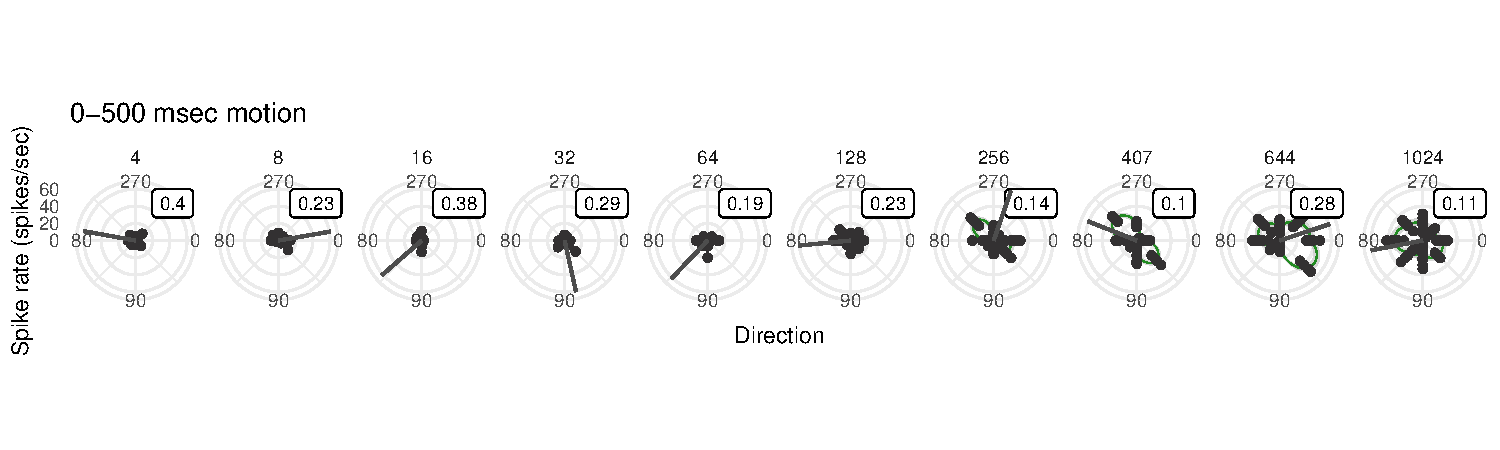
\includegraphics{_main_files/figure-latex/arb-1.pdf}

\hypertarget{construct-a-multi-panel-plot}{%
\section{Construct a multi-panel plot}\label{construct-a-multi-panel-plot}}

We can use the handy \texttt{cowplot} package to construct a multi-panel plot.

\begin{Shaded}
\begin{Highlighting}[]
\NormalTok{cow\_polar }\OtherTok{\textless{}{-}}
  \FunctionTok{plot\_grid}\NormalTok{(naive, cb\_it, cb\_ss, arb,}
            \AttributeTok{nrow =} \DecValTok{1}\NormalTok{)}

\NormalTok{cow\_polar}
\end{Highlighting}
\end{Shaded}

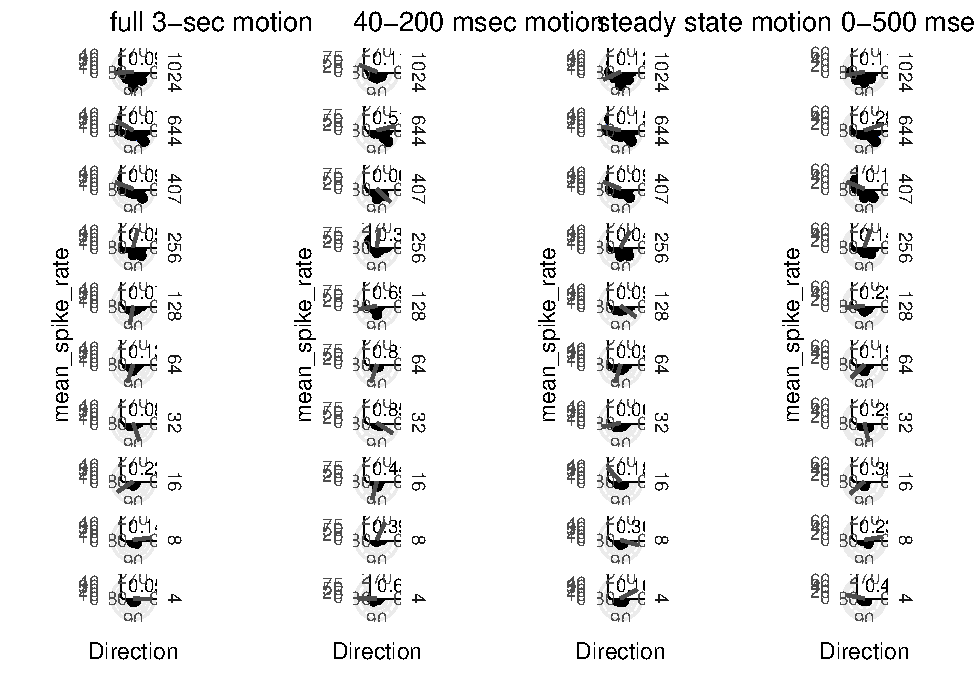
\includegraphics{_main_files/figure-latex/polar_cows-1.pdf}

This plot can also be written directly to \texttt{PDF}.

\begin{Shaded}
\begin{Highlighting}[]
\FunctionTok{pdf}\NormalTok{(}\AttributeTok{file =}
      \FunctionTok{paste0}\NormalTok{(}\StringTok{"./path/to/directory/"}\NormalTok{,}
\NormalTok{             bin10\_basenames[i],}
             \StringTok{"\_polar\_set.pdf"}\NormalTok{),}
    \AttributeTok{width =} \DecValTok{22}\NormalTok{, }\AttributeTok{height =} \DecValTok{17}\NormalTok{,}
    \AttributeTok{pagecentre =} \ConstantTok{TRUE}\NormalTok{, }\AttributeTok{colormodel =} \StringTok{"srgb"}\NormalTok{)}
\FunctionTok{plot}\NormalTok{(cow\_polar)}
\FunctionTok{dev.off}\NormalTok{()}
\end{Highlighting}
\end{Shaded}

\hypertarget{spatiotemporal-tuning}{%
\chapter{Spatiotemporal tuning}\label{spatiotemporal-tuning}}

Coming soon

\hypertarget{histological-verification}{%
\chapter{Histological verification}\label{histological-verification}}

Test post, please ignore

\hypertarget{direct-embedding-method}{%
\subsection{Direct embedding method:}\label{direct-embedding-method}}

\begin{figure}
\centering
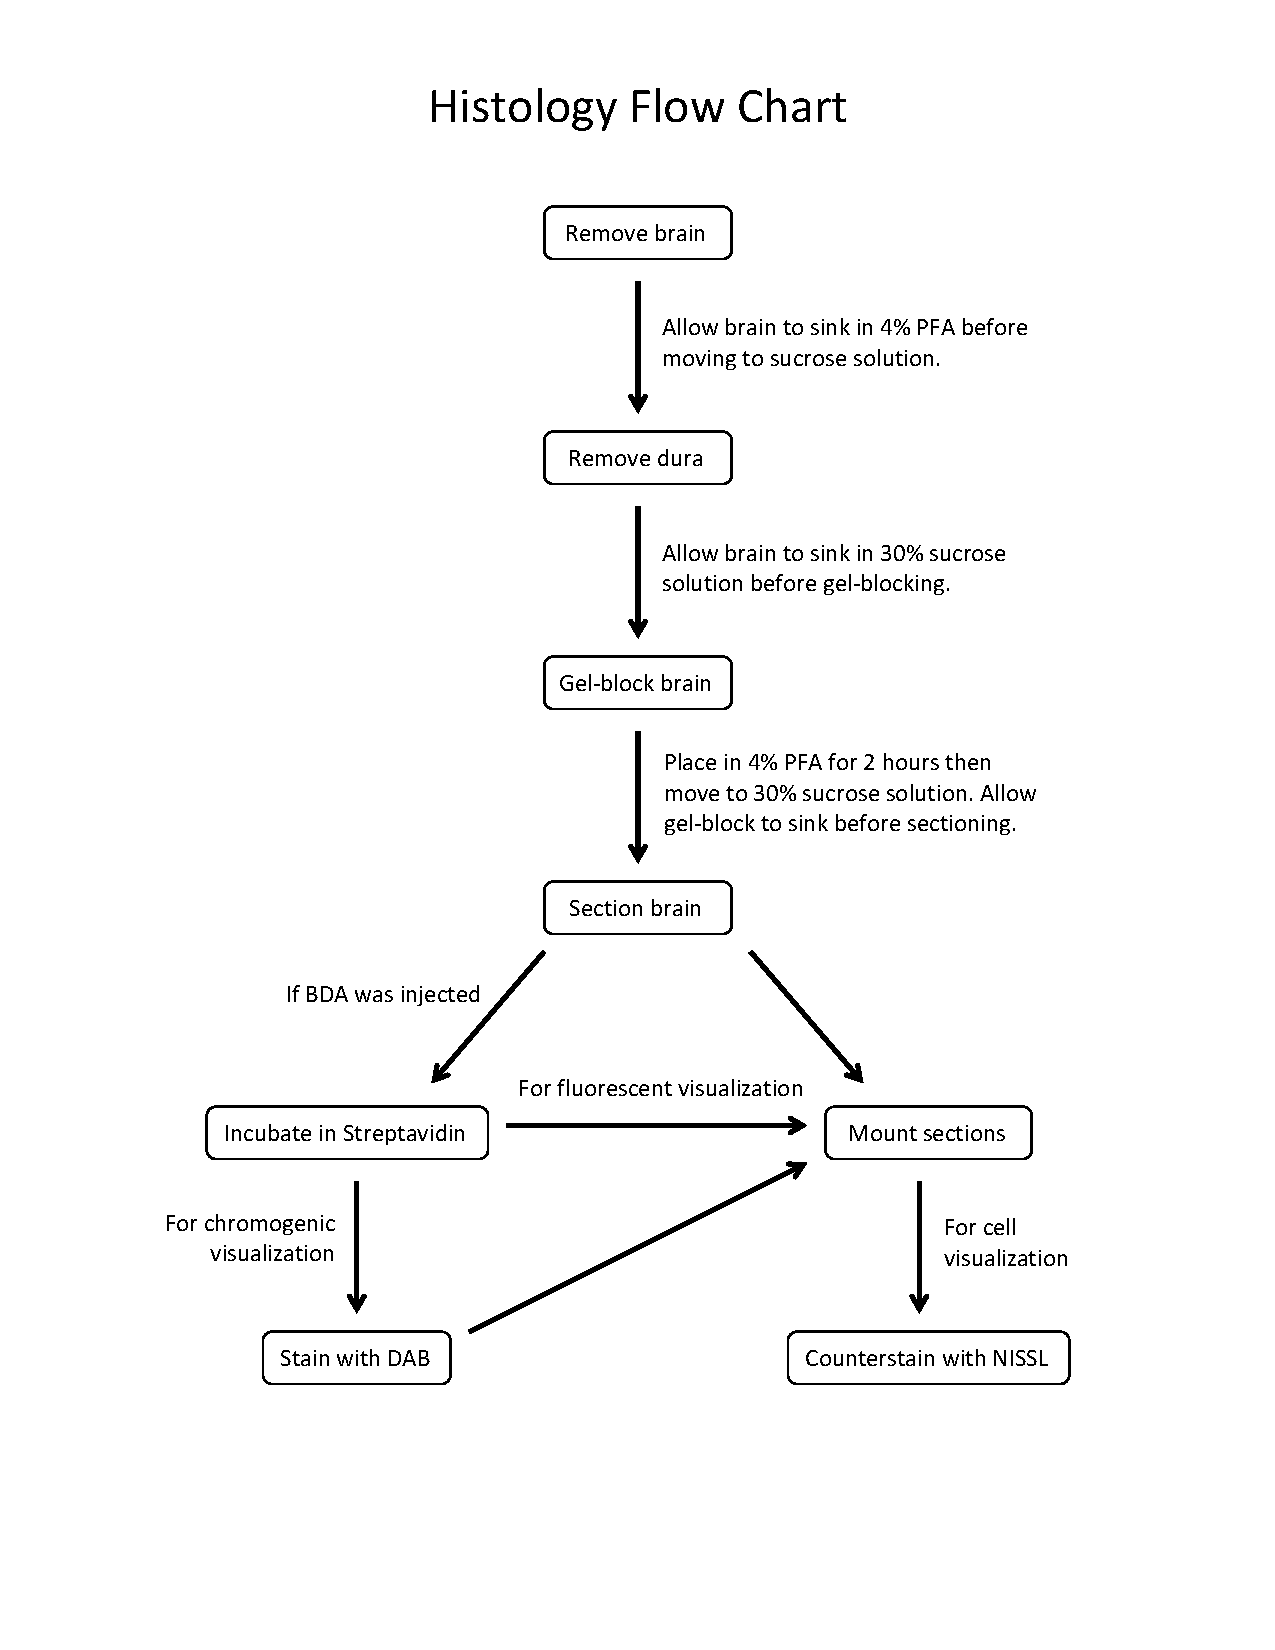
\includegraphics[width=1\textwidth,height=4.16667in]{./histology-flow-chart.pdf}
\caption{Flowchart}
\end{figure}

\hypertarget{hotlinking-method}{%
\subsection{Hotlinking method:}\label{hotlinking-method}}

\href{https://raw.githubusercontent.com/flightlab/ephys_fundamental_plots/master/histology-flow-chart.pdf}{Flowchart link}

  \bibliography{book.bib,packages.bib}

\end{document}
